\documentclass[10pt,conference,compsoc]{IEEEtran}

\usepackage{amsmath}
\usepackage{bm}
\usepackage{colortbl}
\usepackage{datetime}
\usepackage{fancyhdr}
\usepackage{float}
\PassOptionsToPackage{hyphens}{url}
  \usepackage[colorlinks=true,allcolors=blue]{hyperref}
\usepackage{import}
\usepackage{listings}
\usepackage{tabulary}
\usepackage{tikz}

% Load after hyperref
\usepackage[style=super,nonumberlist,toc]{glossaries}
\usepackage[notlof, notlot, nottoc]{tocbibind}
\usepackage{tocloft}

\definecolor{lightblue}{rgb}{0.78,0.918,0.992}

% Set styles for TikZ objects
\usetikzlibrary{arrows, positioning, shapes}
\tikzstyle{block} = [draw, fill=lightblue, rectangle, minimum height=3em, minimum width=4em]
\tikzstyle{sum} = [draw, circle, node distance=1cm]
\tikzstyle{arrow} = [arrows=->, black, align=right]
\tikzstyle{branch} = [circle, inner sep=0pt, minimum size=1mm, fill=black,
    draw=black]

\lstdefinestyle{customMatlab}{
  language=Matlab,
  breaklines=true,
  xleftmargin=0.125in,
  basicstyle=\footnotesize\ttfamily,
  keywordstyle=\color{blue},
  morekeywords=[2]{1}, keywordstyle=[2]{\color{black}},
  identifierstyle=\color{black},
  stringstyle=\color[RGB]{170, 55, 241},
  commentstyle=\color[RGB]{28, 172, 0},
  showstringspaces=false,
  emph=[1]{for,end,break},emphstyle=[1]\color{red},
}

\lstdefinestyle{customcpp}{
  belowcaptionskip=1\baselineskip,
  breaklines=true,
  xleftmargin=0.125in,
  language=C++,
  showstringspaces=false,
  basicstyle=\footnotesize\ttfamily,
  keywordstyle=\color[RGB]{128, 128, 0},
  commentstyle=\color[RGB]{0, 128, 0},
  identifierstyle=\color{black},
  stringstyle=\color[RGB]{0, 128, 0},
}

\newcommand{\includecode}[2][c]{%
  \lstinputlisting[escapechar=, style=custom#1]{#2}
}

\newcommand{\mtx}[1] {\bm #1}

% Set up snippet environment
\newcommand{\listsnippetsname}{\Large List of Snippets}
\newlistof{snippets}{los}{\listsnippetsname}
\cftsetindents{snippets}{\parindent}{1.5\parindent}
\newenvironment{snippet}{
  \renewcommand{\caption}[1]{
    \refstepcounter{snippets}
    \begin{center}
      \par\noindent{\footnotesize Snippet \thesnippets. ##1}
    \end{center}
    \addcontentsline{los}{snippets}
      {\protect \numberline{\thesnippets}{\ignorespaces ##1}}
  }
}
{\par\noindent}

\newdateformat{monthdayyeardate}{%
  \monthname[\THEMONTH]~\THEDAY, \THEYEAR}

% Disable automatic indent and provide \indent command
\newlength\tindent
\setlength{\tindent}{\parindent}
\setlength{\parindent}{0pt}
\renewcommand{\indent}{\hspace*{\tindent}}

% Paper header
\pagestyle{fancy}
\lhead{Practical Guide to State-space Control}
\rhead{\thepage}
\lfoot{}
\rfoot{}
\fancyfoot[C]{}  % remove normal page numbers

\allowdisplaybreaks


\newglossaryentry{controller}{
  name={controller},
  description={Used in positive or negative feedback with a plant to bring about
    a desired system state by driving the difference between a reference signal
    and the output to zero}}
\newglossaryentry{control law}{
  name={control law},
  description={Also known as control policy, is a mathematical formula used by
  the controller to determine the input u that is sent to the plant. This
  control law is designed to drive the system from its current state to some
  other desired state}}
\newglossaryentry{discretization}{
  name={discretization},
  description={The process by which a continuous (e.g., analog) system or
  controller design is converted to discrete (e.g., digital)}}
\newglossaryentry{disturbance}{
  name={disturbance},
  description={An external force acting on a system that isn't included in the
    system's model}}
\newglossaryentry{disturbance rejection}{
  name={disturbance rejection},
  description={The quality of a feedback control system to compensate for
    external forces to reach a desired reference}}
\newglossaryentry{error}{
  name={error},
  description={Reference minus input}}
\newglossaryentry{gain margin}{
  name={gain margin},
  description={See section \ref{sec:gain-phase-margin} on gain and phase
    margin}}
\newglossaryentry{input}{
  name={input},
  description={An input to the plant (hence the name) that can be used to change
  the plant's state}}
\newglossaryentry{model}{
  name={model},
  description={A set of mathematical equations that reflects some aspect of a
    physical system's behavior}}
\newglossaryentry{noise immunity}{
  name={noise immunity},
  description={The quality of a system to have its performance or stability
    unaffected by noise in the outputs (see also: \gls{robustness})}}
\newglossaryentry{open-loop gain}{
  name={open-loop gain},
  description={The gain directly from the input to the output, ignoring loops}}
\newglossaryentry{output}{
  name={output},
  description={Measurements from sensors}}
\newglossaryentry{output-based control}{
  name={output-based control},
  description={Controls the system's state via the outputs}}
\newglossaryentry{phase margin}{
  name={phase margin},
  description={See section \ref{sec:gain-phase-margin} on gain and phase
    margin}}
\newglossaryentry{plant}{
  name={plant},
  description={The system or collection of actuators being controlled}}
\newglossaryentry{realization}{
  name={realization},
  description={In systems theory, this is an implementation of a given
  input-output behavior as a state-space model}}
\newglossaryentry{reference}{
  name={reference},
  description={The desired state}}
\newglossaryentry{reference tracking}{
  name={state tracking},
  description={The ability of a feedback control system to make the state follow
    the reference}}
\newglossaryentry{robustness}{
  name={robustness},
  description={The quality of a feedback control system to remain stable in
    response to disturbances and uncertainty}}
\newglossaryentry{state}{
  name={state},
  description={A characteristic of a system (e.g., velocity) that can be used to
    determine the system's future behavior}}
\newglossaryentry{state feedback}{
  name={state feedback},
  description={Uses state instead of output in feedback}}
\newglossaryentry{steady-state error}{
  name={steady-state error},
  description={Error after system reaches equilibrium}}
\newglossaryentry{stochastic process}{
  name={stochastic process},
  description={A process whose model is partially or completely defined by
    random variables}}
\newglossaryentry{system}{
  name={system},
  description={Maps inputs to outputs through linear combination of states}}
\newglossaryentry{time-invariant}{
  name={time-invariant},
  description={The system's fundamental response does not change over time}}
\newglossaryentry{unity feedback}{
  name={unity feedback},
  description={A feedback network in a control system diagram with a feedback
    gain of 1}}

\makeglossaries

\begin{document}
% Front matter
\pagenumbering{roman}
\begin{titlepage}
  \begin{center}
    \vspace*{1cm}

    \Huge
    \textbf{Practical Guide to State-space Control}

    \vspace{0.5cm}
    \LARGE
    Graduate-level control theory for high schoolers

    \vspace{1.5cm}

    \textbf{Tyler Veness} \\

    \vspace{1.5cm}
    \normalsize
    Generated on \monthdayyeardate\today \\
    \url{https://github.com/calcmogul/state-space-guide}

    \vfill

    \vspace{0.8cm}

    %\begin{figure}[H]
    %  \centering
    %  \def\svgwidth{0.25\columnwidth}
    %  \import{figs/}{wpilib.pdf_tex}
    %\end{figure}
  \end{center}

  \vfill


  \vspace{0.8cm}
\end{titlepage}
\thispagestyle{empty}  % no page number on title sheet

% Table of contents
\pagenumbering{roman}
\renewcommand\contentsname{Table of Contents}
\tableofcontents
\listoffigures
\listoftables
\listofsnippets
\thispagestyle{empty}  % no page number on table of contents sheet
\clearpage
\pagenumbering{arabic}

\chapterimage{preface.jpg}{Flower bush near Spencer's Market in Santa Maria, CA}

\chapter*{Preface}
\addcontentsline{toc}{chapter}{\textcolor{themecolor}{Preface}}

\section*{Motivation}

I am the software mentor for a FIRST Robotics Competition (FRC) team. My
responsibilities for that include teaching programming, software engineering
practices, and applications of control theory. The curriculum I developed so far
(located at \url{https://csweb.frc3512.com/ci/}) teaches rookies enough to be
minimally competitive, but many of the more advanced sections are incomplete. It
provides no formal avenues of growth for veteran students.

Also, out of a six week build season, the software team usually only gets a few
days with the completed robot due to poor build schedule management. This leads
to two problems. First, two days is only enough time to verify basic software
functionality, not test and tune feedback controllers. Second, this is also the
first time the robot's electromechanical systems have been tested after
integration, so any issues that arise consume valuable software integration time
while the team traces the problem to a mechanical, electrical, or software
cause.

This book expands my curriculum to cover control theory topics I have learned in
my graduate-level engineering classes at University of California, Santa Cruz.
It introduces state-space controllers and serves as a practical guide for
formulating and implementing them. Since state-space control utilizes a system
model, both problems mentioned earlier can be addressed. Basic software
functionality can be tested against it and feedback controllers can be tuned
automatically based on system constraints. This allows software teams to test
their work much earlier in the build season in a controlled environment as well
as save time during feedback controller design, implementation, and testing.

I originally started writing this book because I felt that the topic wasn't
difficult, but the information for it wasn't easily accessible. When I was a
high school robotics team member, I had to learn everything from scratch through
various internet sources and eventually from college courses as part of my
bachelor's degree. Control theory has a certain beauty to it, and I want more
people to appreciate it the way I do. Therefore, my goal is to make the learning
process quicker and easier for the team members who come after me by collating
all the relevant information.

\section*{Intended audience}

This guide is intended to make an advanced engineering topic approachable so it
can be applied by those who aren't experts in control theory. My intended
audience is high school students who are members of a FIRST Robotics Competition
team. As such, they will likely have passing knowledge of PID control and have
basic proficiency in programming. This guide will will expand their incomplete
understanding of control theory to include the fundamentals of classical control
theory, enough linear algebra to understand the notation and mechanics of modern
control, and finally how to apply modern control to design challenges they
regularly see in their FRC robots from year to year.

\section*{Acknowledgements}

I would like to thank my controls engineering instructors Dejan Milutinovi\'c
and Gabriel Elkaim of University of California, Santa Cruz. They taught their
classes from a pragmatic perspective focused on application and intuition that I
appreciated. I would also like to thank Dejan Milutinovi\'c for introducing me
to the field of control theory and both of my instructors for teaching me what
it means to be a controls engineer.

Thanks to Austin Schuh from FRC team 971 for providing the final continuous
state-space models used in the examples section.

\cleardoublepage


% Main body
\pagenumbering{arabic}
\section{Introduction}

Recall from linear \gls{system} theory that we defined \glspl{system} as having
the following form:

\begin{align*}
  \dot{\mtx{x}} &= \mtx{A}\mtx{x} + \mtx{B}\mtx{u} + \mtx{\Gamma}\mtx{w} \\
  \mtx{y} &= \mtx{C}\mtx{x} + \mtx{D}\mtx{u} + \mtx{v}
\end{align*}

In this equation, $\mtx{A}$ and $\mtx{B}$ are constant matrices, which means
they are both time-invariant and linear (all transformations on the \gls{system}
\gls{state} are linear ones, and those transformations remain the same for all
time). In nonlinear and time-variant \glspl{system}, the \gls{state} evolution
and \gls{output} are defined by arbitrary functions of the current \glspl{state}
and \glspl{input}.

\begin{align*}
  \dot{\mtx{x}} &= f(\mtx{x}, \mtx{u}, \mtx{w}) \\
  \mtx{y} &= h(\mtx{x}, \mtx{u}, \mtx{v})
\end{align*}

Nonlinear functions come up regularly when attempting to control the \gls{pose}
of a vehicle in the global coordinate frame instead of the vehicle's rotating
local coordinate frame. Converting from one to the other requires applying a
rotation matrix, which consists of sine and cosine operations. These functions
are nonlinear.

\chapterimage{control-system-basics.jpg}{On trail between McHenry Library and Media Theater at UCSC}

\chapter{Control system basics}

\renewcommand*{\chapterpath}{\partpath/control-system-basics}
\section{What is gain?}
\index{gain}

\Gls{gain} is a proportional value that shows the relationship between the
magnitude of an input signal to the magnitude of an output signal at
steady-state. Many \glspl{system} contain a method by which the gain can be
altered, providing more or less ``power" to the \gls{system}.

Figure \ref{fig:input_output_gain} shows a \gls{system} with a hypothetical
input and output. Since the output is twice the amplitude of the input, the
\gls{system} has a gain of $2$.
\begin{bookfigure}
  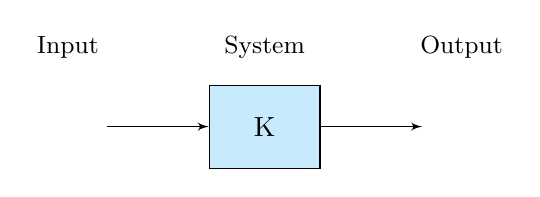
\begin{tikzpicture}[auto, >=latex']
    % \draw [help lines] (-4,-2) grid (4,2);

    % Input
    \drawtimeplot{-2.5cm}{0cm}{0.125cm}{0.44375cm}{0.6 * cos(40 * deg(\x))}
    \draw (-2.5,1) node {\small Input};

    \node [block] (sys) {K};
    \draw (0,1) node {\small System};

    % Output
    \drawtimeplot{2.5cm}{0cm}{0.125cm}{0.44375cm}{1.2 * cos(40* deg(\x))}
    \draw (2.5,1) node {\small Output};

    % Arrows between input/output and system
    \draw[->] (-2,0) -- (sys);
    \draw[->] (sys) -- (2,0);
  \end{tikzpicture}

  \caption{Demonstration of system with a gain of $K = 2$}
  \label{fig:input_output_gain}
\end{bookfigure}

\section{Block diagrams}
\index{block diagrams}

When designing or analyzing a \gls{control system}, it is useful to model it
graphically. Block diagrams are used for this purpose. They can be manipulated
and simplified systematically (see appendix
\ref{ch:simplifying_block_diagrams}). Figure \ref{fig:gain_nomenclature} is an
example of one.

\begin{bookfigure}
  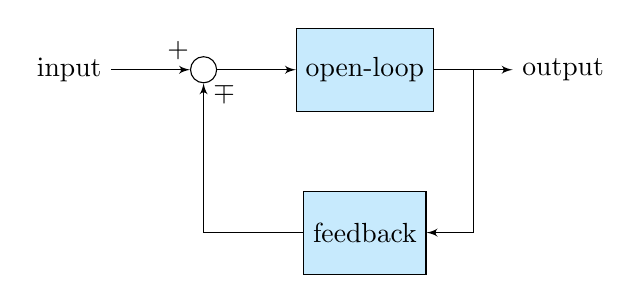
\begin{tikzpicture}[auto, >=latex']
    % Place the blocks
    \node [name=input] {input};
    \node [sum, right=of input] (sum) {};
    \node [block, right=of sum] (P1) {open-loop};
    \node [right=of P1] (output) {output};
    \node [block, below=of P1] (P2) {feedback};

    % Connect the nodes
    \draw [arrow] (input) -- node[pos=0.85] {$+$} (sum);
    \draw [arrow] (sum) -- node {} (P1);
    \draw [arrow] (P1) -- node[name=y] {} (output);
    \draw [arrow] (y) |- (P2);
    \draw [arrow] (P2) -| node[pos=0.97, right] {$\mp$} (sum);
  \end{tikzpicture}

  \caption{Block diagram with nomenclature}
  \label{fig:gain_nomenclature}
\end{bookfigure}

The \gls{open-loop gain} is the total gain from the sum node at the input (the
circle) to the output branch. This would be the \gls{system}'s gain if the
feedback loop was disconnected. The \gls{feedback gain} is the total gain from
the output back to the input sum node. A sum node's output is the sum of its
inputs.

Figure \ref{fig:feedback_block_diagram} is a block diagram with more formal
notation in a feedback configuration.

\begin{bookfigure}
  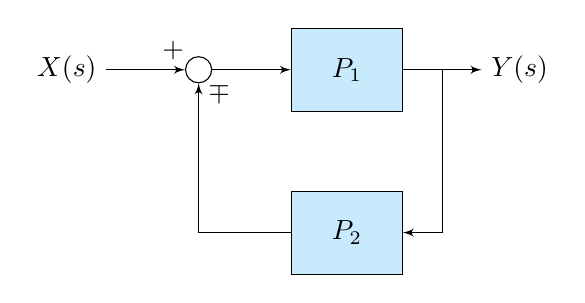
\begin{tikzpicture}[auto, >=latex']
    % Place the blocks
    \node [name=input] {$X(s)$};
    \node [sum, right=of input] (sum) {};
    \node [block, right=of sum] (P1) {$P_1$};
    \node [right=of P1] (output) {$Y(s)$};
    \node [block, below=of P1] (P2) {$P_2$};

    % Connect the nodes
    \draw [arrow] (input) -- node[pos=0.85] {$+$} (sum);
    \draw [arrow] (sum) -- node {} (P1);
    \draw [arrow] (P1) -- node[name=y] {} (output);
    \draw [arrow] (y) |- (P2);
    \draw [arrow] (P2) -| node[pos=0.97, right] {$\mp$} (sum);
  \end{tikzpicture}

  \caption{Feedback block diagram}
  \label{fig:feedback_block_diagram}
\end{bookfigure}

$\mp$ means ``minus or plus" where a minus represents negative feedback.

\section{Why feedback control?}

Let's say we are controlling a DC motor. With just a
\glslink{model}{mathematical model} and knowledge of all current \glspl{state}
of the \gls{system} (i.e., angular velocity), we can predict all future
\glspl{state} given the future voltage \glspl{input}. Why then do we need
feedback control? If the \gls{system} is \glslink{disturbance}{disturbed} in any
way that isn't modeled by our equations, like a load was applied to the
armature, or voltage sag in the rest of the circuit caused the commanded voltage
to not match the actual applied voltage, the angular velocity of the motor will
deviate from the \gls{model} over time.

To combat this, we can take measurements of the \gls{system} and the environment
to detect this deviation and account for it. For example, we could measure the
current position and estimate an angular velocity from it. We can then give the
motor corrective commands as well as steer our \gls{model} back to reality. This
feedback allows us to account for uncertainty and be
\glslink{robustness}{robust} to it.


\chapterimage{review-of-pid.jpg}{Treeline by Crown/Merril bus stop at UCSC}

\chapter{Review of PID controller mathematics}

\section{PID basics and theory}

Negative feedback loops drive the difference between the \gls{reference} and
\gls{output} to zero.

\textbf{Proportional} gain compensates for current \gls{error}. \\
\textbf{Integral} gain compensates for past error (i.e.,
\gls{steady-state error}). \\
\textbf{Derivative} gain compensates for future error by slowing controller down
  if error decreases over time.

\begin{figure}[H]
  \centering

  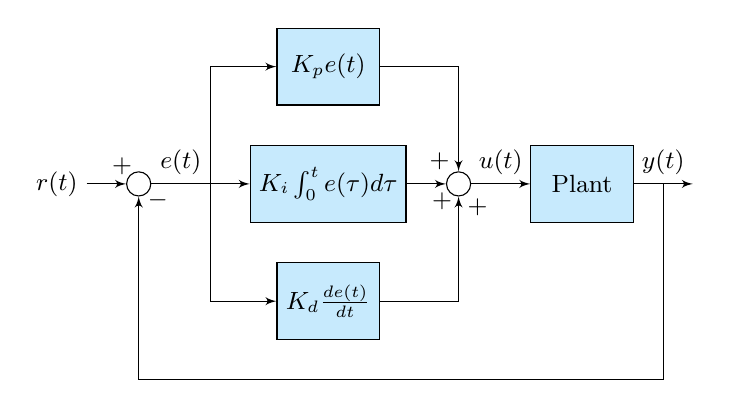
\begin{tikzpicture}[auto, >=latex']
    \fontsize{9pt}{10pt}

    % Place the blocks
    \node [name=input] {$r(t)$};
    \node [sum, right=0.5cm of input] (errorsum) {};
    \node [coordinate, right=0.75cm of errorsum] (branch) {};
    \node [block, right=0.5cm of branch] (I) { $K_i \int_0^t e(\tau) d\tau$ };
    \node [block, above=0.5cm of I] (P) { $K_p e(t)$ };
    \node [block, below=0.5cm of I] (D) { $K_d \frac{de(t)}{dt}$ };
    \node [sum, right=0.5cm of I] (ctrlsum) {};
    \node [block, right=0.75cm of ctrlsum] (plant) {Plant};
    \node [right=0.75cm of plant] (output) {};
    \node [coordinate, below=0.5cm of D] (measurements) {};

    % Connect the nodes
    \draw [arrow] (input) -- node[pos=0.9] {$+$} (errorsum);
    \draw [-] (errorsum) -- node {$e(t)$} (branch);
    \draw [arrow] (branch) |- (P);
    \draw [arrow] (branch) -- (I);
    \draw [arrow] (branch) |- (D);
    \draw [arrow] (P) -| node[pos=0.95, left] {$+$} (ctrlsum);
    \draw [arrow] (I) -- node[pos=0.9, below] {$+$} (ctrlsum);
    \draw [arrow] (D) -| node[pos=0.95, right] {$+$} (ctrlsum);
    \draw [arrow] (ctrlsum) -- node {$u(t)$} (plant);
    \draw [arrow] (plant) -- node [name=y] {$y(t)$} (output);
    \draw [-] (y) |- (measurements);
    \draw [arrow] (measurements) -| node[pos=0.99, right] {$-$} (errorsum);
  \end{tikzpicture}

  \caption{PID controller diagram}
  \label{fig:pid_ctrl_diag}
\end{figure}

\begin{center}
  \renewcommand{\arraystretch}{1.3}
  \begin{tabulary}{\linewidth}{LLLL}
    $r(t)$ & \gls{reference} input & $u(t)$ & control input \\
    $e(t)$ & error & $y(t)$ & \gls{output} \\
  \end{tabulary}
\end{center}

\section{Types of PID controllers}

PID controller inputs of different orders of derivatives, such as position and
velocity, affect the \gls{system} response differently. Below is the standard
form for a position PID controller.

\begin{definition}[Position PID controller]
  \begin{equation}
    u(t) = K_p e(t) + K_i \int_0^t e(\tau) d\tau + K_d \frac{de}{dt}
    \label{def:pos_pid}
  \end{equation}
\end{definition}

If the controller is measuring and controlling velocity instead, the control
input $u(t)$ becomes $\frac{du}{dt}$ and the error $e(t)$ becomes
$\frac{de}{dt}$. Substituting these into equation (\ref{def:pos_pid}) yields

\begin{align}
  \frac{du}{dt} &= K_p \frac{de}{dt} + K_i \int_0^t \frac{de}{d\tau} d\tau +
    K_d \frac{d^2e}{dt^2} \nonumber \\
  \frac{du}{dt} &= K_p \frac{de}{dt} + K_i e(t) + K_d \frac{d^2e}{dt^2}
\end{align}

This shows that the proportional action ($K_p$) of a velocity controller is
caused by the integral action ($K_i$) of a position controller. The derivative
action ($K_i$) of a velocity controller is caused by the proportional action
($K_p$) of a position controller. Integral action ($K_i$) of a velocity
controller has no equivalent in the position formulation. If we were to
implement one, it would use a double integral.

Since for the velocity controller, the proportional term is controlled by an
integral action and the derivative term is controlled by a proportional action,
the coefficients can be relabelled as follows.

\begin{theorem}[Velocity PID controller]
  \begin{equation}
    u = K_p \int_0^t e(\tau) d\tau + K_d e(t)
  \end{equation}
\end{theorem}

Integral control for the velocity is analogous to the throttle pedal on a car.
One must hold the throttle pedal (the control input) at a nonzero value to keep
the car traveling at the reference velocity.

Read \url{https://en.wikipedia.org/wiki/PID_controller} for more information on
PID control theory.

\section{PID control in terms of general control theory}

PID control defines \textit{setpoint} as the desired position and
\textit{process value} as the measured position. Control theory has more general
terms for these: \gls{reference} and \gls{output} respectively.

The derivative term is commonly used to ``slow down" the system if it's already
heading toward the \gls{reference}. We will explore what $K_p$ and $K_d$ are
really doing for a two-state system (position and velocity) and why $K_d$ acts
that way.

First, we will rearrange the equation for a PD controller.

\begin{equation*}
  u = K_p e_k + K_d \frac{e_k - e_{k-1}}{dt}
\end{equation*}

where $u$ is the control input and $e_k$ is the error at timestep $k$. $e_k$ is
defined as $e_k = r_k - x_k$ where $r_k$ is the reference and $x_k$ is the
current state at timestep $k$.

\begin{align*}
  u &= K_p (r_k - x_k) + K_d \frac{(r_k - x_k) - (r_{k-1} - x_{k-1})}{dt} \\
  u &= K_p (r_k - x_k) + K_d \frac{r_k - x_k - r_{k-1} + x_{k-1}}{dt} \\
  u &= K_p (r_k - x_k) + K_d \frac{r_k - r_{k-1} - x_k + x_{k-1}}{dt} \\
  u &= K_p (r_k - x_k) + K_d \frac{(r_k - r_{k-1}) - (x_k - x_{k-1})}{dt} \\
  u &= K_p (r_k - x_k) + K_d \left(\frac{r_k - r_{k-1}}{dt} -
    \frac{x_k - x_{k-1}}{dt}\right)
\end{align*}

Notice how $\frac{r_k - r_{k-1}}{dt}$ is the velocity of the reference. By the
same reasoning, $\frac{x_k - x_{k-1}}{dt}$ is the system's velocity at a given
timestep. That means the $K_d$ term is driving the estimated velocity to the
reference velocity. If the reference is constant, that means the $K_d$ term is
trying to drive the velocity of the system to zero, but it can't because $K_p$
is trying to make the system move and $K_p$ and $K_d$ are controlling the same
actuator. If $K_p$ is larger than $K_d$, one is in effect slowing down the
response of the controller during transients with the hope of decreasing
overshoot and settling time. If one makes $K_d$ much larger than $K_p$, $K_d$
overpowers $K_p$ to bring the system to a stop. However, when the velocity is
low enough, $K_p$ is stronger and starts accelerating the system again. This
oscillatory behavior in the velocity repeats as the system moves toward the
reference.

\section{Limitations of PID control}

PID's heuristic method of tuning is fine when there is no knowledge of the
\gls{system}. However, controllers with much better response can be developed if
a \glslink{model}{dynamical model} of the \gls{system} is known.

\chapterimage{transfer-functions.jpg}{Treeline by Crown/Merril bus stop at UCSC}

\chapter{Transfer functions}

This chapter briefly discusses what transfer functions are, how the locations of
poles and zeroes affect \gls{system response} and stability, and how controllers
affect pole locations. As long as you gain understanding of those concepts,
don't worry too much about not being able to follow the math presented here; we
won't use transfer functions in modern control theory (it's mainly provided for
completeness). This chapter is intended to provide a framework within which to
understand results from the mathematical machinery of modern control as well as
vocabulary to communicate that understanding.

\section{Laplace transform}

For an introduction to Laplace transforms and the geometric intuition behind
transfer functions, we recommend watching Zach Star's video ``What does the
Laplace Transform really tell us? A visual explanation (plus applications)" (21
minutes) \cite{bib:laplace_transform}. An optional, more mathematical
introduction is presented in appendix \ref{ch:laplace-domain-analysis} for
completeness.

\renewcommand*{\chapterpath}{\partpath/transfer-functions}
\section{Parts of a transfer function}

A transfer function maps an input coordinate to an output coordinate in the
Laplace domain. These can be obtained by applying the Laplace transform to a
differential equation and rearranging the terms to obtain a ratio of the output
variable to the input variable. Equation \eqref{eq:transfer_func} is an example
of a transfer function.

\begin{equation} \label{eq:transfer_func}
  H(s) = \frac{\overbrace{(s-9+9i)(s-9-9i)}^{zeroes}}
    {\underbrace{s(s+10)}_{poles}}
\end{equation}

\subsection{Poles and zeroes}

The roots of factors in the numerator of a transfer function are called
\textit{zeroes} because they make the transfer function approach zero. Likewise,
the roots of factors in the denominator of a transfer function are called
\textit{poles} because they make the transfer function approach infinity; on a
3D graph, these look like the poles of a circus tent (see figure
\ref{fig:tf_3d}).

When the factors of the denominator are broken apart using partial fraction
expansion into something like $\frac{A}{s + a} + \frac{B}{s + b}$, the constants
$A$ and $B$ are called residues, which determine how much each pole contributes
to the \gls{system response}.

The factors representing poles are each the Laplace transform of a decaying
exponential\footnote{We are handwaving Laplace transform derivations because
they are complicated and neither relevant nor useful.}. That means the time
domain responses of \glspl{system} comprise decaying exponentials (e.g.,
$y = e^{-t}$).

\begin{svg}{build/\chapterpath/tf_3d}
  \caption{Equation \eqref{eq:transfer_func} plotted in 3D}
  \label{fig:tf_3d}
\end{svg}

\begin{remark}
  Imaginary poles and zeroes always come in complex conjugate pairs (e.g.,
  $-2 + 3i$, $-2 - 3i$).
\end{remark}

\index{stability!poles and zeroes}
The locations of the closed-loop poles in the complex plane determine the
stability of the \gls{system}. Each pole represents a frequency mode of the
\gls{system}, and their location determines how much of each response is induced
for a given input frequency. Figure \ref{fig:impulse_response_poles} shows the
\glspl{impulse response} in the time domain for transfer functions with various
pole locations. They all have an initial condition of $1$.

\begin{bookfigure}
  \begin{tikzpicture}[auto, >=latex']
    % \draw [help lines] (-4,-2) grid (4,4);

    % Draw main axes
    \draw[->] (-4,0) -- (4,0) node[below] {\small Re($\sigma$)};
    \draw[->] (0,-2) -- (0,4) node[right] {\small Im($j\omega$)};

    % Stable: e^-1.75t * cos(1.75wt) (80/3*w for readability)
    \drawtimeplot{-2.125cm}{2.5cm}{0.125cm}{0.44375cm}{
      exp(-1.75 * \x) * cos(80/3 * 1.75 * deg(\x))}
    \drawpole{-1.75cm}{1.75cm}

    % Stable: e^-2.5t
    \drawtimeplot{-2.25cm}{0.75cm}{0.125cm}{0.125cm}{exp(-2 * \x)}
    \drawpole{-2cm}{0cm}

    % Stable: e^-t
    \drawtimeplot{-1.125cm}{-0.75cm}{0.125cm}{0.125cm}{exp(-\x)}
    \drawpole{-1cm}{0cm}

    % Marginally stable: cos(wt) (80/3*w for readability)
    \drawtimeplot{-0.75cm}{1.125cm}{0.125cm}{0.44375cm}{cos(80/3 * deg(\x))}
    \drawpole{0cm}{1cm}

    % Marginally stable cos(2wt) (80/3*w for readability)
    \drawtimeplot{0cm}{2.75cm}{0.125cm}{0.44375cm}{cos(80/3 * 2 * deg(\x))}
    \drawpole{0cm}{2cm}

    % Integrator
    \drawtimeplot{0.25cm}{-0.75cm}{0.125cm}{0.125cm}{1}
    \drawpole{0cm}{0cm}

    % Unstable: e^t
    \drawtimeplot{1.125cm}{0.75cm}{0.125cm}{0.125cm}{exp(\x)}
    \drawpole{1cm}{0cm}

    % Unstable: e^2t
    \drawtimeplot{2.25cm}{-0.75cm}{0.125cm}{0.125cm}{exp(2 * \x)}
    \drawpole{2cm}{0cm}

    % Unstable: e^0.75t * cos(1.75wt) (80/3*w for readability)
    \drawtimeplot{1.5cm}{2.25cm}{0.125cm}{0.44375cm}{
      exp(0.75 * \x) * cos(80/3 * 1.75 * deg(\x))}
    \drawpole{0.75cm}{1.75cm}

    % LHP and RHP labels
    \draw (-3.5,1.5) node {LHP};
    \draw (3.5,1.5) node {RHP};

    % Stable and unstable labels
    \draw (-2.5,3.5) node {\small Stable};
    \draw (2.5,3.5) node {\small Unstable};
  \end{tikzpicture}

  \caption{Impulse response vs pole location}
  \label{fig:impulse_response_poles}
\end{bookfigure}

\begin{booktable}
  \begin{tabular}{|ll|}
    \hline
    \rowcolor{headingbg}
    \textbf{Location} & \textbf{Stability} \\
    \hline
    Left Half-plane (LHP) & Stable \\
    Imaginary axis & Marginally stable \\
    Right Half-plane (RHP) & Unstable \\
    \hline
  \end{tabular}

  \caption{Pole location and stability}
\end{booktable}

When a \gls{system} is stable, its output may oscillate but it converges to
steady-state. When a \gls{system} is marginally stable, its output oscillates at
a constant amplitude forever. When a \gls{system} is unstable, its output grows
without bound.

\subsection{Nonminimum phase zeroes}

While poles in the RHP are unstable, the same is not true for zeroes. They can
be characterized by the \gls{system} initially moving in the wrong direction
before heading toward the \gls{reference}. Since the poles always move toward
the zeroes, zeroes impose a ``speed limit" on the \gls{system response} because
it takes a finite amount of time to move the wrong direction, then change
directions.

One example of this type of \gls{system} is bicycle steering. Try riding a
bicycle without holding the handle bars, then poke the right handle; the bicycle
turns right. Furthermore, if one is holding the handlebars and wants to turn
left, rotating the handlebars counterclockwise will make the bicycle fall toward
the right. The rider has to lean into the turn and overpower the nonminimum
phase dynamics to go the desired direction.

Another example is a Segway. To move forward by some distance, the Segway must
first roll backward to rotate the Segway forward. Once the Segway starts falling
in that direction, it begins rolling forward to avoid falling over until
it reaches the target distance. At that point, the Segway increases its forward
speed to pitch backward and slow itself down. To come to a stop, the Segway
rolls backward again to level itself out.

\subsection{Pole-zero cancellation}
\label{subsec:pole-zero_cancellation}

Pole-zero cancellation occurs when a pole and zero are located at the same place
in the s-plane. This effectively eliminates the contribution of each to the
\gls{system} dynamics. By placing poles and zeroes at various locations (this is
done by placing transfer functions in series), we can eliminate undesired
\gls{system} dynamics. While this may appear to be a useful design tool at
first, there are major caveats. Most of these are due to \gls{model} uncertainty
resulting in poles which aren't in the locations the controls designer expected.

Notch filters are typically used to dampen a specific range of frequencies in
the \gls{system response}. If its band is made too narrow, it can still leave the
undesirable dynamics, but now you can no longer measure them in the response.
They are still happening, but they are what's called \textit{unobservable}.

Never pole-zero cancel unstable or nonminimum phase dynamics. If the \gls{model}
doesn't quite reflect reality, an attempted pole cancellation by placing a
nonminimum phase zero results in the pole still moving to the zero placed next
to it. You have the same dynamics as before, but the pole is also stuck where it
is no matter how much \gls{feedback gain} is applied. For an attempted
nonminimum phase zero cancellation, you have effectively placed an unstable pole
that's unobservable. This means the \gls{system} will be going unstable and
blowing up, but you won't be able to detect this and react to it.

Keep in mind when making design decisions that the \gls{model} likely isn't
perfect. The whole point of feedback control is to be robust to this kind of
uncertainty.

\section{Transfer functions in feedback}

For \glspl{controller} to \glslink{regulator}{regulate} a \gls{system} or
\glslink{tracking}{track} a reference, they must be placed in positive or
negative feedback with the \gls{plant} (whether to use positive or negative
depends on the \gls{plant} in question). Stable feedback loops attempt to make
the \gls{output} equal the \gls{reference}.

\begin{bookfigure}
  \begin{tikzpicture}[auto, >=latex']
    % Place the blocks
    \node [name=input] {$X(s)$};
    \node [sum, right=of input] (sum) {};
    \node [block, right=of sum] (K) {$K$};
    \node [block, right=of K] (G) {$G$};
    \node [right=of G] (output) {$Y(s)$};
    \node [block, below=of $(K)!0.5!(G)$] (H) {$H$};

    % Connect the nodes
    \draw [arrow] (input) -- node[pos=0.85] {$+$} (sum);
    \draw [arrow] (sum) -- node {} (K);
    \draw [arrow] (K) -- node {} (G);
    \draw [arrow] (G) -- node[name=y] {} (output);
    \draw [arrow] (y) |- (H);
    \draw [arrow] (H) -| node[pos=0.97, right] {$-$} (sum);
  \end{tikzpicture}

  \caption{Feedback controller block diagram}
  \label{fig:feedback_controller_block_diagram}

  \begin{figurekey}
    \begin{tabulary}{\linewidth}{LLLL}
      $X(s)$ & input & $H$ & measurement transfer function \\
      $K$ & controller gain & $Y(s)$ & output \\
      $G$ & plant transfer function & & \\
    \end{tabulary}
  \end{figurekey}
\end{bookfigure}

The transfer function of figure \ref{fig:feedback_controller_block_diagram}, a
\gls{control system} diagram with feedback, from input to output is

\begin{equation}
  G_{cl}(s) = \frac{Y(s)}{X(s)} = \frac{KG}{1 + KGH}
\end{equation}

The numerator is the \gls{open-loop gain} and the denominator is one plus the
gain around the feedback loop, which may include parts of the
\gls{open-loop gain} (see appendix \ref{sec:deriv_tf_feedback} for a
derivation). As another example, the transfer function from the input to the
\gls{error} is

\begin{equation}
  G_{cl}(s) = \frac{E(s)}{X(s)} = \frac{1}{1 + KGH}
\end{equation}

The roots of the denominator of $G_{cl}(s)$ are different from those of the
open-loop transfer function $KG(s)$. These are called the closed-loop poles.


\chapterimage{appendices.jpg}{Sunset in an airplane over New Mexico}

\chapter{Laplace domain analysis}
\label{ch:laplace-domain-analysis}

This appendix uses Laplace transforms and transfer functions to analyze
properties of control systems like \gls{steady-state error}.

These case studies cover various aspects of PID control using the algebraic
approach of transfer functions. For this, we'll be using equation
\eqref{eq:pid_tf}, the transfer function for a PID controller.
\begin{equation}
  K(s) = K_p + \frac{K_i}{s} + K_ds \label{eq:pid_tf}
\end{equation}

First, we need to define what Laplace transforms and transfer functions are,
which is rooted in the concept of orthogonal projections.

\renewcommand*{\chapterpath}{\partpath/laplace-domain-analysis}
\section{Projections}

Imagine a two-dimensional Euclidean space $\mathbb{R}^2$ (i.e., the standard x-y
plane). Ordinarily, we notate points in this plane by their components in the
set of basis vectors $\{\hat{i}, \hat{j}\}$, where $\hat{i}$ (pronounced i-hat)
is the unit vector in the $+x$ direction and $\hat{j}$ is the unit vector in the
$+y$ direction.

How do we find the coordinates of a given vector $v$ in this basis? So long as
the basis is \textit{orthogonal} (i.e., the basis vectors are at right angles to
each other), we simply take the \textit{orthogonal projection} of $v$ onto
$\hat{i}$ and $\hat{j}$. Intuitively, this means finding ``the amount of $v$
that points in the direction of $\hat{i}$ or $\hat{j}$". More formally, we can
calculate it with the dot product - the projection of $v$ onto any other vector
$w$ is equal to $\frac{v \cdot w}{|w|}$. (Since $\hat{i}$ and $\hat{j}$ are
\textit{unit vectors}, we can see simply that the coordinates of $v$ are
$v \cdot \hat{i}$ and $v \cdot \hat{j}$. We can also see that ``orthogonal" can
be defined as "has zero dot product".)

But we can use this same process to find the coordinates of $v$ in \textit{any}
orthogonal basis. For example, imagine the basis
$\{\hat{i} + \hat{j}, \hat{i} - \hat{j}\}$ - the coordinates in this basis are
given by $\frac{v \cdot (\hat{i} + \hat{j})}{\sqrt{2}}$ and
$\frac{v \cdot (\hat{i} - \hat{j})}{\sqrt{2}}$. Let us now "unwrap" the formula
for dot product and look a bit more closely.

\begin{equation*}
  \frac{v \cdot (\hat{i} + \hat{j})}{\sqrt{2}} = \frac{1}{\sqrt{2}} \sum_n v_n
    (\hat{i} + \hat{j})_n
\end{equation*}

So, what have we really done to change coordinates? We expanded both $v$ and
$\hat{i} + \hat{j}$ in a basis, multiplied their components, and added them up.

Now the previous example was only a change of coordinates in a
finite-dimensional vector space. However, as we will see, the core idea does not
change much when we move to more complicated structures. Observe the formula for
the Fourier transform.

\begin{equation*}
  \hat{f}(\xi) = \int_{-\infty}^\infty f(x) e^{-2\pi ix \xi} \,dx
    \text{ where } \xi \in \mathbb{R}
\end{equation*}

This is fundamentally the same formula we had before. $f(x)$ has taken the place
of $v_n$, $e^{-2\pi ix \xi}$ has taken the place of $(\hat{i} + \hat{j})_n$, and
the sum over $n$ has turned into an integral over $dx$, but the underlying
concept is the same. To change coordinates in a \textit{function space}, we
simply take the orthogonal projection onto our new basis \textit{functions}. In
the case of the Fourier transform, the function basis is the family of functions
of the form $f(x) = e^{-2\pi ix \xi} \text{ for } \xi \in \mathbb{R}$. Since
these functions are oscillatory at a frequency determined by $\xi$, we can think
of this as a ``frequency basis".

Now, the Laplace transform is somewhat more complicated - as it turns out, the
Fourier basis is orthogonal, so the analogy to the simpler vector space holds
almost-precisely. The Laplace transform is \textit{not} orthogonal, so we can't
interpret it \textit{strictly} as a change of coordinates in the traditional
sense. However, the intuition is the same: we are taking the orthogonal
projection of our original function onto the functions of our new basis set.

\begin{equation*}
  F(s) = \int_0^\infty f(t) e^{-st} \,dt, \text{ where } s \in \mathbb{C}
\end{equation*}

Here, it becomes obvious that the Laplace transform is a \textit{generalization}
of the Fourier transform in that the basis family is strictly larger (we have
allowed the ``frequency" parameter to take \textit{complex} values, as opposed
to merely \textit{real} values). The upshot of this is that the Laplace basis
contains functions that grow and decay, while the Fourier basis does not.

\section{Fourier transform}

The Fourier transform decomposes a function of time into its component
frequencies. Each of these frequencies is part of what's called a
\textit{basis}. These basis waveforms can be multiplied by their respective
contribution amount and summed to produce the original signal (this weighted sum
is called a linear combination). In other words, the Fourier transform provides
a way for us to determine, given some signal, what frequencies can we add
together and in what amounts to produce the original signal.

Think of an Fmajor4 chord which has the notes $F_4$ ($349.23\,Hz$), $A_4$
($440\,Hz$), and $C_4$ ($261.63\,Hz$). The waveform over time looks like figure
\ref{fig:fourier_chord}.

\begin{svg}{build/code/fourier_chord}
  \caption{Frequency decomposition of Fmajor4 chord}
  \label{fig:fourier_chord}
\end{svg}

Notice how this complex waveform can be represented just by three frequencies.
They show up as Dirac delta functions\footnote{The Dirac delta function is zero
everywhere except at the origin. The nonzero region has an infinitesimal width
and has a height such that the area within that region is $1$.} in the frequency
domain with the area underneath them equal to their contribution (see figure
\ref{fig:fourier_chord_fft}).

\begin{svg}{build/code/fourier_chord_fft}
  \caption{Fourier transform of Fmajor4 chord}
  \label{fig:fourier_chord_fft}
\end{svg}

Since Euler's identity states that $e^{i\theta} = \cos\theta + i\sin\theta$, we
can represent frequencies as complex numbers on a number line (we will use
$e^{j\omega} = \cos\omega + j\sin\omega$ for notational consistency going
forward). For example, $400\,Hz$ would be $e^{j400}$. The frequency domain just
uses the complex exponent $400j$.

\subsection{Laplace transform}

The Laplace domain is a generalization of the frequency domain that has the
frequency ($j\omega$) on the imaginary y-axis and a real number on the x-axis,
yielding a two-dimensional coordinate system. We represent coordinates in this
space as a complex number $s = \sigma + j\omega$. The real part $\sigma$
corresponds to the x-axis and the imaginary part $j\omega$ corresponds to the
y-axis (see figure \ref{fig:laplace_domain}).
\begin{bookfigure}
  \begin{tikzpicture}[auto, >=latex']
    %\draw [help lines] (-4,-2) grid (4,4);

    % Draw main axes
    \draw[<->] (-4,0) -- (4,0) node[below] {\small Re($\sigma$)};
    \draw[<->] (0,-3) -- (0,3) node[right] {\small Im($j\omega$)};
  \end{tikzpicture}

  \caption{Laplace domain}
  \label{fig:laplace_domain}
\end{bookfigure}

To extend our analogy of each coordinate being represented by some basis, we now
have the y coordinate representing the oscillation frequency of the
\gls{system response} (the frequency domain) and also the x coordinate
representing the speed at which that oscillation decays and the \gls{system}
converges to zero (i.e., a decaying exponential). Figure
\ref{fig:impulse_response_poles} shows this for various points.

If we move the component frequencies in the Fmajor4 chord example parallel to
the real axis to $\sigma = -25$, the resulting time domain response attenuates
according to the decaying exponential $e^{-25t}$ (see figure
\ref{fig:laplace_chord_attenuating}).
\begin{svg}{build/\sectionpath/laplace_chord_attenuating}
  \caption{Fmajor4 chord at $\sigma = 0$ and $\sigma = -25$}
  \label{fig:laplace_chord_attenuating}
\end{svg}

Note that this explanation as a basis isn't exact because the Laplace basis
isn't orthogonal (that is, the x and y coordinates affect each other and have
cross-talk). In the frequency domain, we had a basis of sine waves that we
represented as delta functions in the frequency domain. Each frequency
contribution was independent of the others. In the Laplace domain, this is not
the case; a pure exponential is $\frac{1}{s - a}$ (a rational function where $a$
is a real number) instead of a delta function. This function is nonzero at
points that aren't actually frequencies present in the time domain. Figure
\ref{fig:laplace_chord_3d} demonstrates this, which shows the Laplace transform
of the Fmajor4 chord plotted in 3D.
\begin{svg}{build/\sectionpath/laplace_chord_3d}
  \caption{Laplace transform of Fmajor4 chord plotted in 3D}
  \label{fig:laplace_chord_3d}
\end{svg}

Notice how the values of the function around each component frequency decrease
according to $\frac{1}{\sqrt{x^2 + y^2}}$ in the $x$ and $y$ directions (in just
the $x$ direction, it would be $\frac{1}{x}$).

\subsection{Laplace transform definition}

The Laplace transform of a function $f(t)$ is defined as
\begin{equation*}
  \mathcal{L}\{f(t)\} = F(s) = \int_0^\infty f(t) e^{-st} \,dt
\end{equation*}

We won't be computing any Laplace transforms by hand using this formula
(everyone in the real world looks these up in a table anyway). Common Laplace
transforms (assuming zero initial conditions) are shown in table
\ref{tab:common_laplace_transforms}. Of particular note are the Laplace
transforms for the derivative, unit step\footnote{The unit step $u(t)$ is
defined as $0$ for $t < 0$ and $1$ for $t \ge 0$.}, and exponential decay. We
can see that a derivative is equivalent to multiplying by $s$, and an integral
is equivalent to multiplying by $\frac{1}{s}$.
\begin{booktable}
  \begin{tabular}{|ccc|}
    \hline
    \rowcolor{headingbg}
    & \textbf{Time domain} & \textbf{Laplace domain} \\
    \hline
    Linearity & $a\,f(t) + b\,g(t)$ & $a\,F(s) + b\,G(s)$ \\
    Convolution & $(f * g)(t)$ & $F(s) \,G(s)$ \\
    Derivative & $f'(t)$ & $s \,F(s)$ \\
    $n^{th}$ derivative & $f^{(n)}(t)$ & $s^n \,F(s)$ \\
    Unit step & $u(t)$ & $\frac{1}{s}$ \\
    Ramp & $t \,u(t)$ & $\frac{1}{s^2}$ \\
    Exponential decay & $e^{-\alpha t} u(t)$ & $\frac{1}{s + \alpha}$ \\
    \hline
  \end{tabular}
  \caption{Common Laplace transforms and Laplace transform properties with zero
    initial conditions}
  \label{tab:common_laplace_transforms}
\end{booktable}

\section{Case study: steady-state error}
\index{steady-state error}

To demonstrate the problem of \gls{steady-state error}, we will use a DC brushed
motor controlled by a velocity PID controller. A DC brushed motor has a transfer
function from voltage ($V$) to angular velocity ($\dot{\theta}$) of
\begin{equation}
  G(s) = \frac{\dot{\Theta}(s)}{V(s)} = \frac{K}{(Js+b)(Ls+R)+K^2}
\end{equation}

First, we'll try controlling it with a P controller defined as
\begin{equation*}
  K(s) = K_p
\end{equation*}

When these are in unity feedback, the transfer function from the input voltage
to the error is
\begin{align*}
  \frac{E(s)}{V(s)} &= \frac{1}{1 + K(s)G(s)} \\
  E(s) &= \frac{1}{1 + K(s)G(s)} V(s) \\
  E(s) &= \frac{1}{1 + (K_p) \left(\frac{K}{(Js+b)(Ls+R)+K^2}\right)} V(s) \\
  E(s) &= \frac{1}{1 + \frac{K_p K}{(Js+b)(Ls+R)+K^2}} V(s)
\end{align*}

The steady-state of a transfer function can be found via
\begin{equation}
  \lim_{s\to0} sH(s)
\end{equation}

since steady-state has an input frequency of zero.
\begin{align}
  e_{ss} &= \lim_{s\to0} sE(s) \nonumber \\
  e_{ss} &= \lim_{s\to0} s \frac{1}{1 + \frac{K_p K}{(Js+b)(Ls+R)+K^2}} V(s)
    \nonumber \\
  e_{ss} &= \lim_{s\to0} s \frac{1}{1 + \frac{K_p K}{(Js+b)(Ls+R)+K^2}}
    \frac{1}{s} \nonumber \\
  e_{ss} &= \lim_{s\to0} \frac{1}{1 + \frac{K_p K}{(Js+b)(Ls+R)+K^2}}
    \nonumber \\
  e_{ss} &= \frac{1}{1 + \frac{K_p K}{(J(0)+b)(L(0)+R)+K^2}} \nonumber \\
  e_{ss} &= \frac{1}{1 + \frac{K_p K}{bR+K^2}} \label{eq:ss_nonzero}
\end{align}

Notice that the \gls{steady-state error} is nonzero. To fix this, an integrator
must be included in the controller.
\begin{equation*}
  K(s) = K_p + \frac{K_i}{s}
\end{equation*}

The same steady-state calculations are performed as before with the new
controller.
\begin{align*}
  \frac{E(s)}{V(s)} &= \frac{1}{1 + K(s)G(s)} \\
  E(s) &= \frac{1}{1 + K(s)G(s)} V(s) \\
  E(s) &= \frac{1}{1 + \left(K_p + \frac{K_i}{s}\right)
    \left(\frac{K}{(Js+b)(Ls+R)+K^2}\right)} \left(\frac{1}{s}\right) \\
  e_{ss} &= \lim_{s\to0} s \frac{1}{1 + \left(K_p + \frac{K_i}{s}\right)
    \left(\frac{K}{(Js+b)(Ls+R)+K^2}\right)} \left(\frac{1}{s}\right) \\
  e_{ss} &= \lim_{s\to0} \frac{1}{1 + \left(K_p + \frac{K_i}{s}\right)
    \left(\frac{K}{(Js+b)(Ls+R)+K^2}\right)} \\
  e_{ss} &= \lim_{s\to0} \frac{1}{1 + \left(K_p + \frac{K_i}{s}\right)
    \left(\frac{K}{(Js+b)(Ls+R)+K^2}\right)} \frac{s}{s} \\
  e_{ss} &= \lim_{s\to0} \frac{s}{s + \left(K_p s + K_i\right)
    \left(\frac{K}{(Js+b)(Ls+R)+K^2}\right)} \\
  e_{ss} &= \frac{0}{0 + (K_p (0) + K_i)
    \left(\frac{K}{(J(0)+b)(L(0)+R)+K^2}\right)} \\
  e_{ss} &= \frac{0}{K_i \frac{K}{bR+K^2}}
\end{align*}

The denominator is nonzero, so $e_{ss} = 0$. Therefore, an integrator is
required to eliminate \gls{steady-state error} in all cases for this
\gls{model}.

It should be noted that $e_{ss}$ in equation \eqref{eq:ss_nonzero} approaches
zero for $K_p = \infty$. This is known as a bang-bang controller. In practice,
an infinite switching frequency cannot be achieved, but it may be close enough
for some performance specifications.

\section{Case study: flywheel PID control}
\index{PID control!flywheel (modern control)}

PID controllers typically control voltage to a motor in FRC independent of the
equations of motion of that motor. For position PID control, large values of
$K_p$ can lead to overshoot and $K_d$ is commonly used to reduce overshoots.
Let's consider a flywheel controlled with a standard PID controller. Why
wouldn't $K_d$ provide damping for velocity overshoots in this case?

PID control is designed to control second-order and first-order \glspl{system}
well. It can be used to control a lot of things, but struggles when given higher
order \glspl{system}. It has three degrees of freedom. Two are used to place the
two poles of the \gls{system}, and the third is used to remove steady-state
error. With higher order \glspl{system} like a one input, seven \gls{state}
\gls{system}, there aren't enough degrees of freedom to place the \gls{system}'s
poles in desired locations. This will result in poor control.

The math for PID doesn't assume voltage, a motor, etc. It defines an output
based on derivatives and integrals of its input. We happen to use it for motors
because it actually works pretty well for it because motors are second-order
\glspl{system}.

The following math will be in continuous time, but the same ideas apply to
discrete time. This is all assuming a velocity controller.

Our simple motor model hooked up to a mass is
\begin{align}
  V &= IR + \frac{\omega}{K_v} \label{eq:steady-state_error_ss_flywheel_1} \\
  \tau &= I K_t \label{eq:steady-state_error_ss_flywheel_2} \\
  \tau &= J \frac{d\omega}{dt} \label{eq:steady-state_error_ss_flywheel_3}
\end{align}

For an explanation of where these equations come from, read section
\ref{sec:dc_brushed_motor}.

First, we'll solve for $\frac{d\omega}{dt}$ in terms of $V$.

Substitute equation \eqref{eq:steady-state_error_ss_flywheel_2} into equation
\eqref{eq:steady-state_error_ss_flywheel_1}.
\begin{align}
  V &= IR + \frac{\omega}{K_v} \nonumber \\
  V &= \left(\frac{\tau}{K_t}\right) R + \frac{\omega}{K_v} \nonumber
  \intertext{Substitute in equation
    \eqref{eq:steady-state_error_ss_flywheel_3}.}
  V &= \frac{\left(J \frac{d\omega}{dt}\right)}{K_t} R + \frac{\omega}{K_v}
    \nonumber \\
  \intertext{Solve for $\frac{d\omega}{dt}$.}
  V &= \frac{J \frac{d\omega}{dt}}{K_t} R + \frac{\omega}{K_v} \nonumber \\
  V - \frac{\omega}{K_v} &= \frac{J \frac{d\omega}{dt}}{K_t} R \nonumber \\
  \frac{d\omega}{dt} &= \frac{K_t}{JR} \left(V - \frac{\omega}{K_v}\right)
    \nonumber \\
  \underbrace{\frac{d\omega}{dt}}_{\dot{\mat{x}}} &=
    \underbrace{-\frac{K_t}{JRK_v}}_{\mat{A}} \underbrace{\omega}_{\mat{x}} +
    \underbrace{\frac{K_t}{JR}}_{\mat{B}} \underbrace{V}_{\mat{u}}
\end{align}

There's one stable open-loop pole at $-\frac{K_t}{JRK_v}$. Let's try a simple P
controller.
\begin{align*}
  \mat{u} &= \mat{K} (\mat{r} - \mat{x}) \\
  V &= K_p (\omega_{goal} - \omega)
\end{align*}

Closed-loop models have the form
$\dot{\mat{x}} = (\mat{A} - \mat{B}\mat{K})\mat{x} + \mat{B}\mat{K}\mat{r}$.
Therefore, the closed-loop poles are the eigenvalues of
$\mat{A} - \mat{B}\mat{K}$.
\begin{align*}
  \dot{\mat{x}} &= (\mat{A} - \mat{B}\mat{K})\mat{x} + \mat{B}\mat{K}\mat{r}
    \\
  \dot{\omega} &= \left(\left(-\frac{K_t}{JRK_v}\right) -
    \left(\frac{K_t}{JR}\right)(K_p)\right)\omega +
    \left(\frac{K_t}{JR}\right)(K_p)(\omega_{goal}) \\
  \dot{\omega} &= -\left(\frac{K_t}{JRK_v} + \frac{K_t K_p}{JR}\right)\omega +
    \frac{K_t K_p}{JR}\omega_{goal}
\end{align*}

This closed-loop flywheel model has one pole at
$-\left(\frac{K_t}{JRK_v} + \frac{K_t K_p}{JR}\right)$. It therefore only needs
one P controller to place that pole anywhere on the real axis. A derivative
term is unnecessary on an ideal flywheel. It may compensate for unmodeled
dynamics such as accelerating projectiles slowing the flywheel down, but that
effect may also increase recovery time; $K_d$ drives the acceleration to zero in
the undesired case of negative acceleration as well as well as the actually
desired case of positive acceleration.

This analysis assumes that the motor is well coupled to the mass and that the
time constant of the inductor is small enough that it doesn't factor into the
motor equations. The latter is a pretty good assumption, as shown by the slight
wiggle in figure \ref{fig:cs_ss_highfreq_unstable_step} compared to figure
\ref{fig:cs_ss_highfreq_stable_step}. If more mass is added to the motor
armature, the response timescales increase and the inductance matters even less.
\begin{bookfigure}
  \begin{minisvg}{2}{build/figs/highfreq_unstable_step}
    \caption{Step response of second-order DC brushed motor plant augmented with
      position ($L = 230$ μH)}
    \label{fig:cs_ss_highfreq_unstable_step}
  \end{minisvg}
  \hfill
  \begin{minisvg}{2}{build/figs/highfreq_stable_step}
    \caption{Step response of first-order DC brushed motor plant augmented with
      position}
    \label{fig:cs_ss_highfreq_stable_step}
  \end{minisvg}
\end{bookfigure}

Subsection \ref{subsec:input_error_estimation} covers a superior compensation
method that avoids zeroes in the \gls{controller}, doesn't act against the
desired control action, and facilitates better \gls{tracking}.


\chapterimage{linear-algebra.jpg}{Hills by freeway between Santa Maria and Ventura}

\chapter{Linear algebra}

Modern control theory borrows concepts from linear algebra. At first, linear
algebra may appear very abstract, but there are simple geometric intuitions
underlying it. First, watch 3Blue1Brown's preview video for the
\textit{Essence of Linear Algebra} video series (5 minutes)
\cite{bib:linalg_preview}. The goal here is to provide an intuitive, geometric
understanding of linear algebra as a method of linear transformations.

While only a subset of the material from the videos will be presented here, I
highly suggest watching the whole series \cite{bib:essence_of_linalg}.

\section{Vectors}

See the corresponding \textit{Essence of Linear Algebra} video for more (5
minutes) \cite{bib:linalg_vectors}.

\section{Linear combinations, span, and basis vectors}

See the corresponding \textit{Essence of Linear Algebra} video for more (10
minutes) \cite{bib:linalg_linear_combinations}.

\section{Linear transformations and matrices}

See the corresponding \textit{Essence of Linear Algebra} video for more (11
minutes) \cite{bib:linalg_linear_transformations_and_matrices}.

\section{Matrix multiplication as composition}

See the corresponding \textit{Essence of Linear Algebra} video for more (10
minutes) \cite{bib:linalg_matrix_multiplication_as_composition}.

\section{The determinant}

See the corresponding \textit{Essence of Linear Algebra} video for more (10
minutes) \cite{bib:linalg_the_determinant}.

\section{Eigenvectors and eigenvalues}

See the corresponding \textit{Essence of Linear Algebra} video for more (17
minutes) \cite{bib:linalg_eigenvectors_and_eigenvalues}.

\section{Miscellaneous notation}

This book works with two-dimensional matrices. The dimensionality of these
matrices is specified by row first, then column. For example, a matrix with two
rows and three columns would be a two-by-three matrix. A square matrix has the
same number of rows as columns.

The matrix $\mtx{I}$ is known as the identity matrix, which is a square matrix
with ones along its diagonal and zeroes elsewhere. For example

\begin{equation*}
  \left[
  \begin{array}{ccc}
    1 & 0 & 0 \\
    0 & 1 & 0 \\
    0 & 0 & 1
  \end{array}
  \right]
\end{equation*}

The matrix denoted by $\mtx{0}_{m \times n}$ is a matrix filled with zeroes with
$m$ rows and $n$ columns.

The $^T$ in $\mtx{A}^T$ denotes transpose, which flips the matrix across its
diagonal such that the rows become columns and vice versa.

\chapterimage{ss-representation.jpg}{Road near walking trail off of Rice Ranch Road in Santa Maria, CA}

\chapter{State-space representation}

\begin{remark}
  Chapters from here on use Python Control to demonstrate the concepts discussed
  and perform the complex math required. See appendix
  \ref{ch:app-installing-python-control} for how to install it.
\end{remark}

State-space representation models \glspl{system} as a set of \gls{state}, input,
and output variables related by first-order differential equations that describe
how the system's state changes over time given the current \glspl{state} and
inputs.

\section{Benefits over classical output-based control}

The state-space method provides a more convenient and compact way to model and
analyze \glspl{system} with multiple inputs and outputs. For a system with $p$
inputs and $q$ outputs, we would have to write $q \times p$ Laplace transforms
to represent it. Not only is the resulting algebra unwieldy, but it only works
for linear systems with zero initial conditions. State-space representation uses
the time domain instead of the Laplace domain, so it doesn't have this problem.

Students are still taught classical control first because it provides a
framework within which to understand the results we get from the fancy
mathematical machinery of modern control.

\section{What is state-space?}

Recall from last chapter that 2D space has two axes, $x$ and $y$. We represent
locations within this space as a pair of numbers packaged in a vector, and each
coordinate is a measure of how far to move along the corresponding axis.
State-space is a Cartesian coordinate system with an axis for each \gls{state}
variable, and we represent locations within it the same way we do for 2D space:
with a list of numbers in a vector. Each element in the vector corresponds to a
\gls{state} of the \gls{system}.

In addition to the \gls{state}, inputs and outputs are represented as vectors.
Since the mapping from the current states and inputs to the change in state is a
system of equations, it's natural to write it in matrix form.

\section{State-space notation}

Below are the continuous and discrete versions of state-space notation.

\begin{align}
  \dot{\mtx{x}} &= \mtx{A}\mtx{x} + \mtx{B}\mtx{u} \label{eq:ss_ctrl_x} \\
  \mtx{y} &= \mtx{C}\mtx{x} + \mtx{D}\mtx{u} \label{eq:ss_ctrl_y}
\end{align}

\begin{align}
  \mtx{x}_{k+1} &= \mtx{A}\mtx{x}_k + \mtx{B}\mtx{u}_k \label{eq:ssz_ctrl_x} \\
  \mtx{y}_{k+1} &= \mtx{C}\mtx{x}_k + \mtx{D}\mtx{u}_k \label{eq:ssz_ctrl_y}
\end{align}

\begin{center}
  \renewcommand{\arraystretch}{1.3}
  \begin{tabulary}{\linewidth}{LLLL}
    $\mtx{A}$ & system matrix      & $\mtx{x}$ & state vector \\
    $\mtx{B}$ & input matrix       & $\mtx{u}$ & input vector \\
    $\mtx{C}$ & output matrix      & $\mtx{y}$ & output vector \\
    $\mtx{D}$ & feedthrough matrix &  &  \\
  \end{tabulary}
\end{center}

\begin{table}[h]
  \renewcommand{\arraystretch}{1.5}
  \centering
  \begin{tabular}{|ll|ll|}
    \hline
    \rowcolor{headingbg}
    \textbf{Matrix} & \textbf{Rows $\times$ Columns} &
    \textbf{Matrix} & \textbf{Rows $\times$ Columns} \\
    \hline
    $\mtx{A}$ & states $\times$ states & $\mtx{x}$ & states $\times$ 1 \\
    $\mtx{B}$ & states $\times$ inputs & $\mtx{u}$ & inputs $\times$ 1 \\
    $\mtx{C}$ & outputs $\times$ states & $\mtx{y}$ & outputs $\times$ 1 \\
    $\mtx{D}$ & outputs $\times$ inputs &  &  \\
    \hline
  \end{tabular}
  \caption{State-space matrix dimensions}
  \label{tab:ss_matrix_dims}
\end{table}

In the continuous case, the change in state and the output are linear
combinations of the state vector and the input vector. The $\mtx{A}$, $\mtx{B}$,
$\mtx{C}$, and $\mtx{D}$ matrices are used to map the state vector $\mtx{x}$ and
the input vector $\mtx{u}$ to a change in state.

\section{Canonical forms}

There are two canonical forms used to represent state-space \glspl{model}:
controllable canonical form and observable canonical form. They are used to
provide controllability and observability of a system respectively, which are
mathematical duals of each other. That is, the controller and estimator (state
observer) are complementary problems.

\subsection{Controllable canonical form} \label{subsubsec:ctrl-canon}

State controllability implies that it is possible -- by admissible inputs -- to
steer the \glspl{state} from any initial value to any final value within some
finite time window.

\begin{theorem}[Controllable canonical form]
  A continuous \gls{time-invariant} linear state-space \gls{model} is
  controllable if and only if

  \begin{equation}
    \text{rank} \left(
    \begin{bmatrix}
      \mtx{B} & \mtx{A}\mtx{B} & \mtx{A}^2\mtx{B} & \cdots &
      \mtx{A}^{n-1}\mtx{B}
    \end{bmatrix}
    \right) = n
    \label{eq:ctrl_rank}
  \end{equation}

  where rank is the number of linearly independent rows in a matrix and $n$ is
  the number of \gls{state} variables.
\end{theorem}

Given a \gls{system} of the form

\begin{equation} \label{eq:ctrl_obsv_tf}
  G(s) = \frac{n_1 s^3 + n_2 s^2 + n_3 s + n_4}
    {s^4 + d_1 s^3 + d_2 s^2 + d_3 s + d_4}
\end{equation}

the canonical \gls{realization} of it that satisfies equation
(\ref{eq:ctrl_rank}) is

\begin{align}
  \dot{\mtx{x}}(t) &=
  \begin{bmatrix}
    0 & 1 & 0 & 0 \\
    0 & 0 & 1 & 0 \\
    0 & 0 & 0 & 1 \\
    -d_4 & -d_3 & -d_2 & -d_1
  \end{bmatrix}
  \mtx{x}(t) +
  \begin{bmatrix}
    0 \\
    0 \\
    0 \\
    1
  \end{bmatrix}
  \mtx{u}(t) \\
  \mtx{y}(t) &=
  \begin{bmatrix}
    n_4 & n_3 & n_2 & n_1
  \end{bmatrix}
  \mtx{x}(t)
\end{align}

\subsection{Observable canonical form} \label{subsubsec:obsv-canon}

Observability is a measure for how well internal \glspl{state} of a \gls{system}
can be inferred by knowledge of its external outputs. The observability and
controllability of a \gls{system} are mathematical duals (i.e., as
controllability proves that an input is available that brings any initial
\gls{state} to any desired final \gls{state}, observability proves that knowing
an output trajectory provides enough information to predict the initial
\gls{state} of the \gls{system}).

\begin{theorem}[Observable canonical form]
  A continuous \gls{time-invariant} linear state-space \gls{model} is observable
  if and only if

  \begin{equation} \label{eq:obsv_rank}
    \text{rank} \left(
    \begin{bmatrix}
      C \\
      CA \\
      \vdots \\
      CA^{n-1}
    \end{bmatrix}\right) = n
  \end{equation}

  where rank is the number of linearly independent rows in a matrix and $n$ is
  the number of \gls{state} variables.
\end{theorem}

The canonical \gls{realization} of the \gls{system} in equation
(\ref{eq:ctrl_obsv_tf}) that satisfies equation (\ref{eq:obsv_rank}) is

\begin{align}
  \dot{\mtx{x}}(t) &=
  \begin{bmatrix}
    0 & 0 & 0 & -d_4 \\
    1 & 0 & 0 & -d_3 \\
    0 & 1 & 0 & -d_2 \\
    0 & 0 & 1 & -d_1
  \end{bmatrix}
  \mtx{x}(t) +
  \begin{bmatrix}
    n_4 \\
    n_3 \\
    n_2 \\
    n_1
  \end{bmatrix}
  \mtx{u}(t) \\
  \mtx{y}(t) &=
  \begin{bmatrix}
    0 & 0 & 0 & 1
  \end{bmatrix}
  \mtx{x}(t)
\end{align}

\section{Eigenvalues in state-space}

The eigenvalues of the system matrix can be used to determine the stability of a
\gls{system}.

We'd like to know whether the \gls{system} defined by equation
(\ref{eq:ssz_ctrl_x}) operating with the \gls{control law}
$\mtx{u}_k = \mtx{K}(\mtx{r}_k - \mtx{x}_k)$ converges to the \gls{reference}
$\mtx{r}_k$.

\begin{align}
  \mtx{x}_{k+1} &= \mtx{A}\mtx{x}_k + \mtx{B}\mtx{u}_k \nonumber \\
  \mtx{x}_{k+1} &= \mtx{A}\mtx{x}_k + \mtx{B}(\mtx{K}(\mtx{r}_k - \mtx{x}_k))
    \nonumber \\
  \mtx{x}_{k+1} &= \mtx{A}\mtx{x}_k + \mtx{B}\mtx{K}\mtx{r}_k -
    \mtx{B}\mtx{K}\mtx{x}_k \nonumber \\
  \mtx{x}_{k+1} &= \mtx{A}\mtx{x}_k - \mtx{B}\mtx{K}\mtx{x}_k +
    \mtx{B}\mtx{K}\mtx{r}_k \nonumber \\
  \mtx{x}_{k+1} &= (\mtx{A} - \mtx{B}\mtx{K})\mtx{x}_k +
    \mtx{B}\mtx{K}\mtx{r}_k \label{eq:ctrl_eig_calc}
\end{align}

For equation (\ref{eq:ctrl_eig_calc}) to have a bounded output, the eigenvalues
of $\mtx{A} - \mtx{B}\mtx{K}$ must be within the unit circle.

This derivation can be performed for a \gls{state} estimator as well to
determine whether the \gls{state} estimate converges to the true \gls{state}.
Plugging equation (\ref{eq:z_obsv_y}) into equation (\ref{eq:z_obsv_x}) gives

\begin{align*}
  \hat{\mtx{x}}_{k+1} &= \mtx{A}\hat{\mtx{x}}_k + \mtx{B}\mtx{u}_k +
    \mtx{L} (\mtx{y}_k - \hat{\mtx{y}}_k) \\
  \hat{\mtx{x}}_{k+1} &= \mtx{A}\hat{\mtx{x}}_k + \mtx{B}\mtx{u}_k +
    \mtx{L} (\mtx{y}_k - (\mtx{C}\hat{\mtx{x}}_k + \mtx{D}\mtx{u}_k)) \\
  \hat{\mtx{x}}_{k+1} &= \mtx{A}\hat{\mtx{x}}_k + \mtx{B}\mtx{u}_k +
    \mtx{L} (\mtx{y}_k - \mtx{C}\hat{\mtx{x}}_k - \mtx{D}\mtx{u}_k)
\end{align*}

Plugging in equation (\ref{eq:ssz_ctrl_y}) gives

\begin{align*}
  \hat{\mtx{x}}_{k+1} &= \mtx{A}\hat{\mtx{x}}_k + \mtx{B}\mtx{u}_k +
    \mtx{L}((\mtx{C}\mtx{x}_k + \mtx{D}\mtx{u}_k) - \mtx{C}\hat{\mtx{x}}_k -
    \mtx{D}\mtx{u}_k) \\
  \hat{\mtx{x}}_{k+1} &= \mtx{A}\hat{\mtx{x}}_k + \mtx{B}\mtx{u}_k +
    \mtx{L}(\mtx{C}\mtx{x}_k + \mtx{D}\mtx{u}_k - \mtx{C}\hat{\mtx{x}}_k -
    \mtx{D}\mtx{u}_k) \\
  \hat{\mtx{x}}_{k+1} &= \mtx{A}\hat{\mtx{x}}_k + \mtx{B}\mtx{u}_k +
    \mtx{L}(\mtx{C}\mtx{x}_k - \mtx{C}\hat{\mtx{x}}_k) \\
  \hat{\mtx{x}}_{k+1} &= \mtx{A}\hat{\mtx{x}}_k + \mtx{B}\mtx{u}_k +
    \mtx{L}\mtx{C}(\mtx{x}_k - \hat{\mtx{x}}_k)
\end{align*}

Let $E_k = \mtx{x}_k - \hat{\mtx{x}}_k$ be the error in the estimate
$\hat{\mtx{x}}_k$.

\begin{equation*}
  \hat{\mtx{x}}_{k+1} = \mtx{A}\hat{\mtx{x}}_k + \mtx{B}\mtx{u}_k +
    \mtx{L}\mtx{C}\mtx{E}_k
\end{equation*}

Subtracting this from equation (\ref{eq:ssz_ctrl_x}) gives

\begin{align}
  \mtx{x}_{k+1} - \hat{\mtx{x}}_{k+1} &= \mtx{A}\mtx{x}_k + \mtx{B}\mtx{u}_k -
    (\mtx{A}\hat{\mtx{x}}_k + \mtx{B}\mtx{u}_k +
     \mtx{L}\mtx{C}\mtx{E}_k) \nonumber \\
  \mtx{E}_{k+1} &= \mtx{A}\mtx{x}_k + \mtx{B}\mtx{u}_k -
    (\mtx{A}\hat{\mtx{x}}_k + \mtx{B}\mtx{u}_k + \mtx{L}\mtx{C}\mtx{E}_k)
    \nonumber \\
  \mtx{E}_{k+1} &= \mtx{A}\mtx{x}_k + \mtx{B}\mtx{u}_k -
    \mtx{A}\hat{\mtx{x}}_k - \mtx{B}\mtx{u}_k - \mtx{L}\mtx{C}\mtx{E}_k
    \nonumber \\
  \mtx{E}_{k+1} &= \mtx{A}\mtx{x}_k - \mtx{A}\hat{\mtx{x}}_k -
    \mtx{L}\mtx{C}\mtx{E}_k \nonumber \\
  \mtx{E}_{k+1} &= \mtx{A}(\mtx{x}_k - \hat{\mtx{x}}_k) -
    \mtx{L}\mtx{C}\mtx{E}_k \nonumber \\
  \mtx{E}_{k+1} &= \mtx{A}\mtx{E}_k - \mtx{L}\mtx{C}\mtx{E}_k \nonumber \\
  \mtx{E}_{k+1} &= (\mtx{A} - \mtx{L}\mtx{C})\mtx{E}_k \label{eq:obsv_eig_calc}
\end{align}

For equation (\ref{eq:obsv_eig_calc}) to have a bounded output, the eigenvalues
of $\mtx{A} - \mtx{L}\mtx{C}$ must be within the unit circle. These eigenvalues
represent how fast the estimator converges to the true state of the given
\gls{model}. A fast estimator converges quickly while a slow estimator avoids
amplifying noise in the measurements used to produce a state estimate.

The effect of noise can be seen if it is modeled
\glslink{stochastic process}{stochastically} as

\begin{equation*}
  \hat{\mtx{x}}_{k+1} = \mtx{A}\hat{\mtx{x}}_k + \mtx{B}\mtx{u}_k +
    \mtx{L} (\mtx{y}_k - \hat{\mtx{y}}_k) + \mtx{L}\mtx{\nu}_k
\end{equation*}

where $\mtx{\nu}_k$ is the measurement noise. As $\mtx{L}$ increases, the
measurement noise is amplified.

In summary, a controller is stable if the eigenvalues of
$\mtx{A} - \mtx{B}\mtx{K}$ are within the unit circle, and an estimator is
stable if the eigenvalues of $\mtx{A} - \mtx{L}\mtx{C}$ are within the unit
circle.

As stated before, the controller and estimator are dual problems. Controller
gains can be found assuming perfect estimator (i.e., perfect knowledge of all
\glspl{state}). Estimator gains can be found assuming an accurate \gls{model}
and a controller with perfect \gls{tracking}.

\section{Going digital}

The complex plane discussed so far deals with continuous \glspl{system}. In
decades past, \glspl{plant} and controllers were implemented using analog
electronics, which are continuous in nature. Nowadays, microprocessors can be
used to achieve cheaper, less complex controller designs. However,
discretization (the process of converting a design from continuous to digital)
has drawbacks.

\subsection{Phase loss}

Since a microcontroller performs discrete steps, there is phase loss introduced
in the controller. Phase loss is the reduction of phase margin (see section
\ref{sec:gain_phase_margin}) that occurs in digital implementations of feedback
controllers from sampling the continuous system at discrete time intervals. As
the sample rate of the controller decreases, the phase margin decreases rapidly
and will lead to instability if the phase margin reaches zero. Large amounts of
phase loss can make a stable controller in the continuous domain become unstable
in the discrete domain. Here are a few ways to combat this.

\begin{itemize}
  \item Run the controller with a high sample rate.
  \item Designing the controller in the analog domain with enough phase margin
    to compensate for any phase loss that occurs as part of discretization.
  \item Convert the \gls{plant} to the digital domain and design the controller
    completely in the digital domain.
\end{itemize}

\subsection{s-plane to z-plane}

Transfer functions are converted to impulse responses using the Z-transform. The
s-plane's LHP maps to the inside of a unit circle in the z-plane. Table
\ref{tab:s-plane2z-plane} contains a few common points. \\

\begin{table}
  \caption{Mapping from s-plane to z-plane}
  \renewcommand{\arraystretch}{1.3}
  \centering
  \begin{tabular}{|cc|}
    \hline
    \rowcolor{lightblue}
    \textbf{s-plane} & \textbf{z-plane} \\
    \hline
    $(0, 0)$ & $(0, 1)$ \\
    imaginary axis & edge of unit circle \\
    $(0, -\infty)$ & $(0, 0)$ \\
    \hline
  \end{tabular}
  \label{tab:s-plane2z-plane}
\end{table}

You may notice that poles can be placed at $(0, 0)$ in the z-plane. This is
known as a deadbeat controller. An $\rm N^{th}$ order deadbeat controller decays
to the \gls{reference} in N timesteps. While this sounds great, there are other
considerations like actuation effort, \gls{robustness}, and
\gls{noise immunity}. These will be discussed in detail with LQR and LQE.

\subsection{Discretization in state-space}

This process is generally done with computers, but for completeness:

\begin{align}
  \mtx{A}_d &= e^{\mtx{A}_c T} \\
  \mtx{B}_d &= \int_0^T e^{\mtx{A}_c \tau} d\tau \mtx{B}_c \\
  \mtx{C}_d &= \mtx{C}_c \\
  \mtx{D}_d &= \mtx{D}_c
\end{align}

where a subscript of $d$ denotes discrete, a subscript of $c$ denotes
continuous, and $T$ is the sample period for the discrete system.
$e^{\mtx{A}_c T}$ and others are referred to as matrix exponentials. \\

\subsubsection{Computing the matrix exponential}

Let $\mtx{X}$ be an $n \times n$ matrix. The exponential of $\mtx{X}$ denoted by
$e^{\mtx{X}}$ is the $n \times n$ matrix given by the power series below.

\begin{equation}
  e^{\mtx{X}} = \sum_{k=0}^\infty \frac{1}{k!} \mtx{X}^k
\end{equation}

where $\mtx{X}^0$ is defined to be the identity matrix $\mtx{I}$ with the same
dimensions as $\mtx{X}$.

\chapterimage{ss-controllers.jpg}{Night sky above Dufour Street in Santa Cruz, CA}

\chapter{State-space controllers}

When we want to command a \gls{system} to a set of \glspl{state}, we design a
controller with certain \glspl{control law} to do it. PID controllers use the
system \glspl{output} with proportional, integral, and derivative
\glspl{control law}. In state-space, we also have knowledge of the system
\glspl{state} so we can do better.

\renewcommand*{\chapterpath}{\partpath/ss-controllers}
\section{Closed-loop controller}
\index{state-space controllers!discrete closed-loop}

With the \gls{control law} $\mat{u}_k = \mat{K}(\mat{r}_k - \mat{x}_k)$, we can
derive the closed-loop state-space equations. We'll discuss where this
\gls{control law} comes from in subsection \ref{sec:lqr}.

First is the \gls{state} update equation. Substitute the \gls{control law} into
equation \eqref{eq:disc_ss_x}.
\begin{align}
  \mat{x}_{k+1} &= \mat{A}\mat{x}_k + \mat{B}\mat{K}(\mat{r}_k - \mat{x}_k)
    \nonumber \\
  \mat{x}_{k+1} &= \mat{A}\mat{x}_k + \mat{B}\mat{K}\mat{r}_k -
    \mat{B}\mat{K}\mat{x}_k \nonumber \\
  \mat{x}_{k+1} &= (\mat{A} - \mat{B}\mat{K})\mat{x}_k + \mat{B}\mat{K}\mat{r}_k
    \label{eq:disc_ss_ctrl_x}
  \intertext{Now for the \gls{output} equation. Substitute the \gls{control law}
    into equation \eqref{eq:disc_ss_y}.}
  \mat{y}_k &= \mat{C}\mat{x}_k + \mat{D}(\mat{K}(\mat{r}_k - \mat{x}_k))
    \nonumber \\
  \mat{y}_k &= \mat{C}\mat{x}_k + \mat{D}\mat{K}\mat{r}_k -
    \mat{D}\mat{K}\mat{x}_k \nonumber \\
  \mat{y}_k &= (\mat{C} - \mat{D}\mat{K})\mat{x}_k + \mat{D}\mat{K}\mat{r}_k
\end{align}

\index{stability!eigenvalues}
Instead of commanding the \gls{system} to a \gls{state} using the vector
$\mat{u}_k$ directly, we can now specify a vector of desired \glspl{state}
through $\mat{r}_k$ and the \gls{controller} will choose values of $\mat{u}_k$
for us over time to make the \gls{system} converge to the \gls{reference}.

The eigenvalues of $\mat{A} - \mat{B}\mat{K}$ are the poles of the closed-loop
\gls{system}. Therefore, the rate of convergence and stability of the
closed-loop \gls{system} can be changed by moving the poles via the eigenvalues
of $\mat{A} - \mat{B}\mat{K}$. $\mat{A}$ and $\mat{B}$ are inherent to the
\gls{system}, but $\mat{K}$ can be chosen arbitrarily by the controller
designer. For equation \eqref{eq:disc_ss_ctrl_x} to reach steady-state, the
eigenvalues of $\mat{A} - \mat{B}\mat{K}$ must be in the left-half plane.
\begin{booktable}
  \begin{tabular}{|lll|}
    \hline
    \rowcolor{headingbg}
    \textbf{Symbol} & \textbf{Name} & \textbf{Rows $\times$ Columns} \\
    \hline
    $\mat{A}$ & system matrix & states $\times$ states \\
    $\mat{B}$ & input matrix & states $\times$ inputs \\
    $\mat{C}$ & output matrix & outputs $\times$ states \\
    $\mat{D}$ & feedthrough matrix & outputs $\times$ inputs \\
    $\mat{K}$ & controller gain matrix & inputs $\times$ states \\
    $\mat{r}$ & \gls{reference} vector & states $\times$ 1 \\
    $\mat{x}$ & state vector & states $\times$ 1 \\
    $\mat{u}$ & input vector & inputs $\times$ 1 \\
    $\mat{y}$ & output vector & outputs $\times$ 1 \\
    \hline
  \end{tabular}
  \caption{Controller matrix dimensions}
\end{booktable}

\section{Pole placement}
\index{controller design!pole placement}

This is the practice of placing the poles of a closed-loop \gls{system} directly
to produce a desired response. Python Control offers several pole placement
algorithms for generating controller or observer gains from a set of poles.

Since all our applications will be discrete \glspl{system}, we'll place poles in
the discrete domain (the z-plane). The s-plane's LHP maps to the inside of a
unit circle (see figure \ref{fig:s2z_mapping_pp}).
\begin{bookfigure}
  \begin{minisvg}{2}{build/modern-control-theory/discrete-state-space-control/s_plane}
  \end{minisvg}
  \hfill
  \begin{minisvg}{2}{build/modern-control-theory/discrete-state-space-control/z_plane}
  \end{minisvg}
  \caption{Mapping of axes from s-plane (left) to z-plane (right)}
  \label{fig:s2z_mapping_pp}
\end{bookfigure}

Pole placement should only be used if you know what you're doing. It's much
easier to let LQR place the poles for you, which we'll discuss next.

\section{LQR} \label{sec:lqr}
\index{Controller design!LQR}
\index{Optimal control!LQR}

Instead of placing the poles of a closed-loop \gls{system} manually, LQR design
places the poles for us based on acceptable \gls{error} and \gls{control effort}
constraints. ``LQR" stands for ``Linear-Quadratic
\glslink{regulator}{Regulator}". This method of controller design uses a
quadratic function for the cost-to-go defined as the sum of the \gls{error} and
\gls{control effort} over time for the linear \gls{system}
$\dot{\mtx{x}} = \mtx{A}\mtx{x} + \mtx{B}\mtx{u}$.

\begin{equation*}
  J = \int\limits_0^\infty \left(\mtx{x}^T\mtx{Q}\mtx{x} +
    \mtx{u}^T\mtx{R}\mtx{u}\right) dt
\end{equation*}

where $J$ represents a tradeoff between \gls{state} excursion and
\gls{control effort} with the weighting factors $\mtx{Q}$ and $\mtx{R}$. LQR
finds a \gls{control law} $\mtx{u}$ that minimizes the cost function. $\mtx{Q}$
and $\mtx{R}$ slide the cost along a Pareto boundary between state tracking and
\gls{control effort} (see figure \ref{fig:pareto_boundary}). Pareto optimality
for this problem means that an improvement in state \gls{tracking} cannot be
obtained without using more \gls{control effort} to do so. Also, a reduction in
\gls{control effort} cannot be obtained without sacrificing state \gls{tracking}
performance. Pole placement, on the other hand, will have a cost anywhere on,
above, or to the right of the Pareto boundary (no cost can be inside the
boundary).

\begin{svg}{build/code/pareto_boundary}
  \caption{Pareto boundary for LQR}
  \label{fig:pareto_boundary}
\end{svg}

The minimum of LQR's cost function is found by setting the derivative of the
cost function to zero and solving for the \gls{control law} $\mtx{u}$. However,
matrix calculus is used instead of normal calculus to take the derivative.

The feedback \gls{control law} that minimizes $J$, which we'll call the
``optimal control law", is shown in theorem \ref{thm:optimal_control_law}.

\begin{theorem}[Optimal control law]
  \label{thm:optimal_control_law}

  \begin{equation}
    \mtx{u} = -\mtx{K}\mtx{x}
  \end{equation}
\end{theorem}
\index{Controller design!LQR!optimal control law}
\index{Optimal control!LQR!optimal control law}

This means that optimal control can be achieved with simply a set of
proportional gains on all the \glspl{state}. This \gls{control law} will make
all \glspl{state} converge to zero assuming the \gls{system} is controllable. To
converge to nonzero \glspl{state}, a \gls{reference} vector $\mtx{r}$ can be
added to the \gls{state} $\mtx{x}$.

\begin{theorem}[Optimal control law with nonzero reference]
  \begin{equation}
    \mtx{u} = \mtx{K}(\mtx{r} - \mtx{x})
  \end{equation}
\end{theorem}

To use the \gls{control law}, we need knowledge of the full \gls{state} of the
\gls{system}. That means we either have to measure all our \glspl{state}
directly or estimate those we do not measure.

See appendix \ref{sec:deriv_lqr} for how $\mtx{K}$ is calculated in Python. If
the result is finite, the controller is guaranteed to be stable and
\glslink{robustness}{robust} with a \gls{phase margin} of 60 degrees
\cite{bib:lqr_phase_margin}.

\begin{remark}
  LQR design's $\mtx{Q}$ and $\mtx{R}$ matrices don't need \gls{discretization},
  but the $\mtx{K}$ calculated for continuous time and discrete time
  \glspl{system} will be different.
\end{remark}

\subsection{Bryson's rule}
\index{Controller design!LQR!Bryson's rule}
\index{Optimal control!LQR!Bryson's rule}

The next obvious question is what values to choose for $\mtx{Q}$ and $\mtx{R}$.
With Bryson's rule, the diagonals of the $\mtx{Q}$ and $\mtx{R}$ matrices are
chosen based on the maximum acceptable value for each \gls{state} and actuator.
The nondiagonal elements are zero. The balance between $\mtx{Q}$ and $\mtx{R}$
can be slid along the Pareto boundary using a weighting factor $\rho$.

\begin{equation*}
  J = \int\limits_0^\infty \left(\rho \left[
    \left(\frac{x_1}{x_{1,max}}\right)^2 + \ldots +
    \left(\frac{x_n}{x_{n,max}}\right)^2\right] + \left[
    \left(\frac{u_1}{u_{1,max}}\right)^2 + \ldots +
    \left(\frac{u_n}{u_{n,max}}\right)^2\right]\right) dt
\end{equation*}

\begin{equation*}
  \begin{array}{cc}
    \mtx{Q} = \begin{bmatrix}
      \frac{\rho}{x_{1,max}^2} & 0 & \ldots & 0 \\
      0 & \frac{\rho}{x_{2,max}^2} & & \vdots \\
      \vdots & & \ddots & 0 \\
      0 & \ldots & 0 & \frac{\rho}{x_{n,max}^2}
    \end{bmatrix} &
    \mtx{R} = \begin{bmatrix}
      \frac{1}{u_{1,max}^2} & 0 & \ldots & 0 \\
      0 & \frac{1}{u_{2,max}^2} & & \vdots \\
      \vdots & & \ddots & 0 \\
      0 & \ldots & 0 & \frac{1}{u_{n,max}^2}
    \end{bmatrix}
  \end{array}
\end{equation*}

Small values of $\rho$ penalize \gls{control effort} while large values of
$\rho$ penalize \gls{state} excursions. Large values would be chosen in
applications like fighter jets where performance is necessary. Spacecrafts would
use small values to conserve their limited fuel supply.

\section{Case studies of controller design methods}

This example uses the following second-order model for a CIM motor (a DC brushed
motor).

\begin{align*}
  \begin{array}{cccc}
    \mtx{A} = \begin{bmatrix}
      -\frac{b}{J} & \frac{K_t}{J} \\
      -\frac{K_e}{L} & -\frac{R}{L}
    \end{bmatrix} &
    \mtx{B} = \begin{bmatrix}
      0 \\
      \frac{1}{L}
    \end{bmatrix} &
    \mtx{C} = \begin{bmatrix}
      1 & 0
    \end{bmatrix} &
    \mtx{D} = \begin{bmatrix}
      0
    \end{bmatrix}
  \end{array}
\end{align*}

Figure \ref{fig:case_study_pp_lqr} shows the response using poles placed at
$(0.1, 0)$ and $(0.9, 0)$ and LQR with the following cost matrices.

\begin{align*}
  \begin{array}{cc}
    \mtx{Q} = \begin{bmatrix}
      \frac{1}{20^2} & 0 \\
      0 & \frac{1}{40^2}
    \end{bmatrix} &
    \mtx{R} = \begin{bmatrix}
      \frac{1}{12^2}
    \end{bmatrix}
  \end{array}
\end{align*}

\begin{svg}{build/code/case_study_pp_lqr}
  \caption{Second-order CIM motor response with pole placement and LQR}
  \label{fig:case_study_pp_lqr}
\end{svg}

LQR selected poles at $(0.593, 0)$ and $(0.955, 0)$. Notice with pole placement
that as the current pole moves left, the control effort becomes more aggressive.

\input{\chapterpath/ss-observers-and-localization}
\section{Model augmentation}

This section will teach various tricks relating to state-space representation
aimed at demystifying the matrix algebra at play.

\section{Feedforwards}

Feedforwards are used to inject information about either the \gls{system}'s
dynamics (like a \gls{model} does) or the intended movement into a controller.
Feedforward is generally used to handle parts of the control actions we already
know must be applied to make a \gls{system} track a \gls{reference}, then let
the feedback controller correct for at runtime what we do not or cannot know
about the \gls{system}. We will present two ways of implementing feedforward for
\gls{state} feedback.

\subsection{Steady-state feedforward}

Steady-state feedforwards apply the \gls{control effort} required to keep a
\gls{system} at the \gls{reference} if it is no longer moving (i.e., the
\gls{system} is at steady-state). The first steady-state feedforward converts
desired \glspl{output} to desired \glspl{state}.

\begin{equation*}
  \mtx{x}_c = \mtx{N}_x\mtx{y}_c
\end{equation*}

$\mtx{N}_x$ converts desired \glspl{output} $\mtx{y}_c$ to desired \glspl{state}
$\mtx{x}_c$ (also known as $\mtx{r}$). For steady-state, that is

\begin{equation}
  \mtx{x}_{ss} = \mtx{N}_x\mtx{y}_{ss} \label{eq:x_ss}
\end{equation}

The second steady-state feedforward converts the desired \glspl{output}
$\mtx{y}$ to the \gls{control input} required at steady-state.

\begin{equation*}
  \mtx{u}_c = \mtx{N}_u\mtx{y}_c
\end{equation*}

$\mtx{N}_u$ converts the desired \glspl{output} $\mtx{y}$ to the
\gls{control input} $\mtx{u}$ required at steady-state. For steady-state, that
is

\begin{equation}
  \mtx{u}_{ss} = \mtx{N}_u\mtx{y}_{ss} \label{eq:u_ss}
\end{equation}

\subsubsection{Continuous case}

To find the \gls{control input} required at steady-state, set equation
(\ref{eq:ss_ctrl_x}) to zero.

\begin{align*}
  \dot{\mtx{x}} &= \mtx{A}\mtx{x} + \mtx{B}\mtx{u} \\
  \mtx{y} &= \mtx{C}\mtx{x} + \mtx{D}\mtx{u}
\end{align*}

\begin{align*}
  \mtx{0} &= \mtx{A}\mtx{x}_{ss} + \mtx{B}\mtx{u}_{ss} \\
  \mtx{y}_{ss} &= \mtx{C}\mtx{x}_{ss} + \mtx{D}\mtx{u}_{ss}
\end{align*}

\begin{align*}
  \mtx{0} &= \mtx{A}\mtx{N}_x\mtx{y}_{ss} + \mtx{B}\mtx{N}_u\mtx{y}_{ss} \\
  \mtx{y}_{ss} &= \mtx{C}\mtx{N}_x\mtx{y}_{ss} + \mtx{D}\mtx{N}_u\mtx{y}_{ss}
\end{align*}

\begin{align*}
  \begin{bmatrix}
    \mtx{0} \\
    \mtx{y}_{ss}
  \end{bmatrix} &=
  \begin{bmatrix}
    \mtx{A}\mtx{N}_x + \mtx{B}\mtx{N}_u \\
    \mtx{C}\mtx{N}_x + \mtx{D}\mtx{N}_u
  \end{bmatrix}
  \mtx{y}_{ss} \\
  \begin{bmatrix}
    \mtx{0} \\
    \mtx{1}
  \end{bmatrix} &=
  \begin{bmatrix}
    \mtx{A}\mtx{N}_x + \mtx{B}\mtx{N}_u \\
    \mtx{C}\mtx{N}_x + \mtx{D}\mtx{N}_u
  \end{bmatrix} \\
  \begin{bmatrix}
    \mtx{0} \\
    \mtx{1}
  \end{bmatrix} &=
  \begin{bmatrix}
    \mtx{A} & \mtx{B} \\
    \mtx{C} & \mtx{D}
  \end{bmatrix}
  \begin{bmatrix}
    \mtx{N}_x \\
    \mtx{N}_u
  \end{bmatrix} \\
  \begin{bmatrix}
    \mtx{N}_x \\
    \mtx{N}_u
  \end{bmatrix} &=
  \begin{bmatrix}
    \mtx{A} & \mtx{B} \\
    \mtx{C} & \mtx{D}
  \end{bmatrix}^{\dagger}
  \begin{bmatrix}
    \mtx{0} \\
    \mtx{1}
  \end{bmatrix}
\end{align*}

where $^\dagger$ is the Moore-Penrose pseudoinverse.

\subsubsection{Discrete case}

Now, we'll do the same thing for the discrete \gls{system}. To find the
\gls{control input} required at steady-state, set equation (\ref{eq:ssz_ctrl_x})
to zero.

\begin{align*}
  \mtx{x}_{k+1} &= \mtx{A}\mtx{x}_k + \mtx{B}\mtx{u}_k \\
  \mtx{y}_k &= \mtx{C}\mtx{x}_k + \mtx{D}\mtx{u}_k
\end{align*}

\begin{align*}
  \mtx{x}_{ss} &= \mtx{A}\mtx{x}_{ss} + \mtx{B}\mtx{u}_{ss} \\
  \mtx{y}_{ss} &= \mtx{C}\mtx{x}_{ss} + \mtx{D}\mtx{u}_{ss}
\end{align*}

\begin{align*}
  \mtx{0} &= (\mtx{A} - \mtx{I})\mtx{x}_{ss} + \mtx{B}\mtx{u}_{ss} \\
  \mtx{y}_{ss} &= \mtx{C}\mtx{x}_{ss} + \mtx{D}\mtx{u}_{ss}
\end{align*}

\begin{align*}
  \mtx{0} &= (\mtx{A} - \mtx{I})\mtx{N}_x\mtx{y}_{ss} +
    \mtx{B}\mtx{N}_u\mtx{y}_{ss} \\
  \mtx{y}_{ss} &= \mtx{C}\mtx{N}_x\mtx{y}_{ss} + \mtx{D}\mtx{N}_u\mtx{y}_{ss}
\end{align*}

\begin{align*}
  \begin{bmatrix}
    \mtx{0} \\
    \mtx{y}_{ss}
  \end{bmatrix} &=
  \begin{bmatrix}
    (\mtx{A} - \mtx{I})\mtx{N}_x + \mtx{B}\mtx{N}_u \\
    \mtx{C}\mtx{N}_x + \mtx{D}\mtx{N}_u
  \end{bmatrix}
  \mtx{y}_{ss} \\
  \begin{bmatrix}
    \mtx{0} \\
    \mtx{1}
  \end{bmatrix} &=
  \begin{bmatrix}
    (\mtx{A} - \mtx{I})\mtx{N}_x + \mtx{B}\mtx{N}_u \\
    \mtx{C}\mtx{N}_x + \mtx{D}\mtx{N}_u
  \end{bmatrix} \\
  \begin{bmatrix}
    \mtx{0} \\
    \mtx{1}
  \end{bmatrix} &=
  \begin{bmatrix}
    \mtx{A} - \mtx{I} & \mtx{B} \\
    \mtx{C} & \mtx{D}
  \end{bmatrix}
  \begin{bmatrix}
    \mtx{N}_x \\
    \mtx{N}_u
  \end{bmatrix} \\
  \begin{bmatrix}
    \mtx{N}_x \\
    \mtx{N}_u
  \end{bmatrix} &=
  \begin{bmatrix}
    \mtx{A} - \mtx{I} & \mtx{B} \\
    \mtx{C} & \mtx{D}
  \end{bmatrix}^{\dagger}
  \begin{bmatrix}
    \mtx{0} \\
    \mtx{1}
  \end{bmatrix}
\end{align*}

where $^\dagger$ is the Moore-Penrose pseudoinverse.

\subsubsection{Deriving steady-state input}

Now, we'll find an expression that uses $\mtx{N}_x$ and $\mtx{N}_u$ to convert
the \gls{reference} $\mtx{r}$ to a \gls{control input} feedforward
$\mtx{u}_{ff}$. Let's start with equation (\ref{eq:x_ss}).

\begin{align*}
  \mtx{x}_{ss} &= \mtx{N}_x \mtx{y}_{ss} \\
  \mtx{N}_x^\dagger \mtx{x}_{ss} &= \mtx{y}_{ss}
\end{align*}

Now substitute this into equation (\ref{eq:u_ss}).

\begin{align*}
  \mtx{u}_{ss} &= \mtx{N}_u \mtx{y}_{ss} \\
  \mtx{u}_{ss} &= \mtx{N}_u (\mtx{N}_x^\dagger \mtx{x}_{ss}) \\
  \mtx{u}_{ss} &= \mtx{N}_u \mtx{N}_x^\dagger \mtx{x}_{ss}
\end{align*}

$\mtx{u}_{ss}$ and $\mtx{x}_{ss}$ are also known as $\mtx{u}_{ff}$ and $\mtx{r}$
respectively.

\begin{align*}
  \mtx{u}_{ff} = \mtx{N}_u \mtx{N}_x^\dagger \mtx{r}
\end{align*}

So all together, we get theorem \ref{thm:steady-state_ff}.

\index{Feedforward!steady-state feedforward}
\begin{theorem}[Steady-state feedforward]
  \label{thm:steady-state_ff}

  \begin{align}
    &\text{Continuous:} \nonumber \\
    &\begin{bmatrix}
      \mtx{N}_x \\
      \mtx{N}_u
    \end{bmatrix} =
    \begin{bmatrix}
      \mtx{A} & \mtx{B} \\
      \mtx{C} & \mtx{D}
    \end{bmatrix}^{\dagger}
    \begin{bmatrix}
      \mtx{0} \\
      \mtx{1}
    \end{bmatrix} \\
    &\text{Discrete:} \nonumber \\
    &\begin{bmatrix}
      \mtx{N}_x \\
      \mtx{N}_u
    \end{bmatrix} =
    \begin{bmatrix}
      \mtx{A} - \mtx{I} & \mtx{B} \\
      \mtx{C} & \mtx{D}
    \end{bmatrix}^{\dagger}
    \begin{bmatrix}
      \mtx{0} \\
      \mtx{1}
    \end{bmatrix}
  \end{align}

  \begin{equation}
    \mtx{u}_{ff} = \mtx{N}_u \mtx{N}_x^\dagger \mtx{r}
  \end{equation}

  In the augmented matrix, $\mtx{B}$ should contain one column corresponding to
  an actuator and $\mtx{C}$ should contain one row whose \gls{output} will be
  driven by that actuator. More than one actuator or output can be included in
  the computation at once, but the result won't be the same as if they were
  computed independently and summed afterward.

  After computing the feedforward for each actuator-output pair, the respective
  collections of $\mtx{N}_x$ and $\mtx{N}_u$ matrices can summed to produce the
  combined feedforward.
\end{theorem}

If the augmented matrix in theorem \ref{thm:steady-state_ff} is square (number
of \glspl{input} = number of \glspl{output}), the normal matrix inverse can be
used instead.

\subsection{Two-state feedforward}

Let's start with the equation for the \gls{reference} dynamics

\begin{equation*}
  \mtx{r}_{k+1} = \mtx{A}\mtx{r}_k + \mtx{B}\mtx{u}_{ff}
\end{equation*}

where $\mtx{u}_{ff}$ is the feedforward input. Note that this feedforward
equation does not and should not take into account any feedback terms. We want
to find the optimal $\mtx{u}_{ff}$ such that we minimize the \gls{tracking}
error between $\mtx{r}_{k+1}$ and $\mtx{r}_k$.

\begin{equation*}
  \mtx{r}_{k+1} - \mtx{A}\mtx{r}_k = \mtx{B}\mtx{u}_{ff}
\end{equation*}

To solve for $\mtx{u}_{ff}$, we need to take the inverse of the nonsquare matrix
$\mtx{B}$. This isn't possible, but we can find the pseudoinverse given some
constraints on the \gls{state} \gls{tracking} error and \gls{control effort}. To
find the optimal solution for these sorts of trade-offs, one can define a cost
function and attempt to minimize it. To do this, we'll first solve the
expression for $\mtx{0}$.

\begin{equation*}
  \mtx{0} = \mtx{B}\mtx{u}_{ff} - (\mtx{r}_{k+1} - \mtx{A}\mtx{r}_k)
\end{equation*}

This expression will be the \gls{state} \gls{tracking} cost we use in our cost
function.

Our cost function will use an $H_2$ norm with $\mtx{Q}$ as the \gls{state} cost
matrix with dimensionality $states \times states$ and $\mtx{R}$ as the
\gls{control input} cost matrix with dimensionality $inputs \times inputs$.

\begin{equation*}
  \mtx{J} = (\mtx{B}\mtx{u}_{ff} - (\mtx{r}_{k+1} - \mtx{A}\mtx{r}_k))^T \mtx{Q}
    (\mtx{B}\mtx{u}_{ff} - (\mtx{r}_{k+1} - \mtx{A}\mtx{r}_k)) +
    \mtx{u}_{ff}^T\mtx{R}\mtx{u}_{ff}
\end{equation*}

\begin{remark}
  $\mtx{r}_{k+1} - \mtx{A}\mtx{r}_k$ will only return a nonzero vector if the
  \gls{reference} isn't following the \gls{system} dynamics. If it is, the
  feedback controller already compensates for it. This feedforward compensates
  for any unmodeled dynamics reflected in how the \gls{reference} is changing
  (or not changing). In the case of a constant \gls{reference}, the feedforward
  opposes any \gls{system} dynamics that would change the \gls{state} over time.
\end{remark}

The following theorems will be needed to find the minimum of $\mtx{J}$.

\begin{theorem}
  \label{thm:partial_xax}

  $\frac{\partial \mtx{x}^T\mtx{A}\mtx{x}}{\partial\mtx{x}} =
    2\mtx{A}\mtx{x}$ where $\mtx{A}$ is symmetric.
\end{theorem}

\begin{theorem}
  \label{thm:partial_ax_b}

  $\frac{\partial (\mtx{A}\mtx{x} + \mtx{b})^T\mtx{C}
    (\mtx{D}\mtx{x} + \mtx{e})}{\partial\mtx{x}} =
    \mtx{A}^T\mtx{C}(\mtx{D}\mtx{x} + \mtx{e}) + \mtx{D}^T\mtx{C}^T
    (\mtx{A}\mtx{x} + \mtx{b})$
\end{theorem}

\begin{corollary}
  \label{cor:partial_ax_b}

  $\frac{\partial (\mtx{A}\mtx{x} + \mtx{b})^T\mtx{C}
    (\mtx{A}\mtx{x} + \mtx{b})}{\partial\mtx{x}} =
    2\mtx{A}^T\mtx{C}(\mtx{A}\mtx{x} + \mtx{b})$ where $\mtx{C}$ is symmetric.

  Proof:
  \begin{align*}
    \frac{\partial (\mtx{A}\mtx{x} + \mtx{b})^T\mtx{C}
      (\mtx{A}\mtx{x} + \mtx{b})}{\partial\mtx{x}} &=
      \mtx{A}^T\mtx{C}(\mtx{A}\mtx{x} + \mtx{b}) + \mtx{A}^T\mtx{C}^T
      (\mtx{A}\mtx{x} + \mtx{b}) \\
    \frac{\partial (\mtx{A}\mtx{x} + \mtx{b})^T\mtx{C}
      (\mtx{A}\mtx{x} + \mtx{b})}{\partial\mtx{x}} &=
      (\mtx{A}^T\mtx{C} + \mtx{A}^T\mtx{C}^T)(\mtx{A}\mtx{x} + \mtx{b})
  \end{align*}

  $\mtx{C}$ is symmetric, so

  \begin{align*}
    \frac{\partial (\mtx{A}\mtx{x} + \mtx{b})^T\mtx{C}
      (\mtx{A}\mtx{x} + \mtx{b})}{\partial\mtx{x}} &=
      (\mtx{A}^T\mtx{C} + \mtx{A}^T\mtx{C})(\mtx{A}\mtx{x} + \mtx{b}) \\
    \frac{\partial (\mtx{A}\mtx{x} + \mtx{b})^T\mtx{C}
      (\mtx{A}\mtx{x} + \mtx{b})}{\partial\mtx{x}} &=
      2\mtx{A}^T\mtx{C}(\mtx{A}\mtx{x} + \mtx{b})
  \end{align*}
\end{corollary}

Given theorem \ref{thm:partial_xax} and corollary \ref{cor:partial_ax_b}, find
the minimum of $\mtx{J}$ by taking the partial derivative with respect to
$\mtx{u}_{ff}$ and setting the result to $\mtx{0}$.

\begin{align*}
  \frac{\partial\mtx{J}}{\partial\mtx{u}_{ff}} &= 2\mtx{B}^T\mtx{Q}
    (\mtx{B}\mtx{u}_{ff} - (\mtx{r}_{k+1} - \mtx{A}\mtx{r}_k)) +
    2\mtx{R}\mtx{u}_{ff} \\
  \mtx{0} &= 2\mtx{B}^T\mtx{Q}
    (\mtx{B}\mtx{u}_{ff} - (\mtx{r}_{k+1} - \mtx{A}\mtx{r}_k)) +
    2\mtx{R}\mtx{u}_{ff} \\
  \mtx{0} &= \mtx{B}^T\mtx{Q}
    (\mtx{B}\mtx{u}_{ff} - (\mtx{r}_{k+1} - \mtx{A}\mtx{r}_k)) +
    \mtx{R}\mtx{u}_{ff} \\
  \mtx{0} &= \mtx{B}^T\mtx{Q}\mtx{B}\mtx{u}_{ff} -
    \mtx{B}^T\mtx{Q}(\mtx{r}_{k+1} - \mtx{A}\mtx{r}_k) + \mtx{R}\mtx{u}_{ff} \\
  \mtx{B}^T\mtx{Q}\mtx{B}\mtx{u}_{ff} + \mtx{R}\mtx{u}_{ff} &=
    \mtx{B}^T\mtx{Q}(\mtx{r}_{k+1} - \mtx{A}\mtx{r}_k) \\
  (\mtx{B}^T\mtx{Q}\mtx{B} + \mtx{R})\mtx{u}_{ff} &=
    \mtx{B}^T\mtx{Q}(\mtx{r}_{k+1} - \mtx{A}\mtx{r}_k) \\
  \mtx{u}_{ff} &= (\mtx{B}^T\mtx{Q}\mtx{B} + \mtx{R})^{-1}
    \mtx{B}^T\mtx{Q}(\mtx{r}_{k+1} - \mtx{A}\mtx{r}_k)
\end{align*}

\begin{theorem}[Two-state feedforward]
  \label{thm:two-state_ff}

  \begin{align}
    &\mtx{u}_{ff} = \mtx{K}_{ff} (\mtx{r}_{k+1} - \mtx{A}\mtx{r}_k) \\
    &\text{where } \mtx{K}_{ff} =
      (\mtx{B}^T\mtx{Q}\mtx{B} + \mtx{R})^{-1}\mtx{B}^T\mtx{Q}
  \end{align}
\end{theorem}
\index{Feedforward!two-state feedforward}
\index{Optimal control!two-state feedforward}

If \gls{control effort} is considered inexpensive, $\mtx{R} \ll \mtx{Q}$ and
$\mtx{u}_{ff}$ approaches corollary \ref{cor:two-state_ff_no_r}.

\begin{corollary}[Two-state feedforward with inexpensive control effort]
  \label{cor:two-state_ff_no_r}

  \begin{align}
    &\mtx{u}_{ff} = \mtx{K}_{ff} (\mtx{r}_{k+1} - \mtx{A}\mtx{r}_k) \\
    &\text{where } \mtx{K}_{ff} =
      (\mtx{B}^T\mtx{Q}\mtx{B})^{-1}\mtx{B}^T\mtx{Q}
  \end{align}
\end{corollary}

\begin{remark}
  If the cost matrix $\mtx{Q}$ isn't included in the cost function (that is,
  $\mtx{Q}$ is set to the identity matrix), $\mtx{K}_{ff}$ becomes the
  Moore-Penrose pseudoinverse of $\mtx{B}$ given by
  $\mtx{B}^\dagger = (\mtx{B}^T\mtx{B})^{-1}\mtx{B}^T$.
\end{remark}

\subsection{Case studies of feedforwards}

\subsubsection{Second-order CIM motor model}

Each feedforward implementation has advantages. The steady-state feedforward
allows using specific actuators to maintain the \gls{reference} at steady-state.
The two-state feedforward doesn't support this, but can be used for
\gls{reference} \gls{tracking} as well with the same tuning parameters as LQR
design. Figure \ref{fig:case_study_ff1} shows both types of feedforwards applied
to a second-order CIM motor model.

\begin{svg}{build/code/case_study_ff1}
  \caption{Second-order CIM motor response with various feedforwards}
  \label{fig:case_study_ff1}
\end{svg}

The two-state feedforward isn't as effective in figure \ref{fig:case_study_ff1}
because the $\mtx{R}$ matrix penalized \gls{control effort}. If the $\mtx{R}$
cost matrix is removed from the two-state feedforward calculation, the
\gls{reference} \gls{tracking} is much better (see figure
\ref{fig:case_study_ff2}).

\begin{svg}{build/code/case_study_ff2}
  \caption{Second-order CIM motor response with two-state feedforwards}
  \label{fig:case_study_ff2}
\end{svg}

\section{Integral control}
\label{sec:integral_control}

A common way of implementing integral control is to add an additional
\gls{state} that is the integral of the \gls{error} of the variable intended to
have zero \gls{steady-state error}.

There are two drawbacks to this method. First, there is integral windup on a
unit \gls{step input}. That is, the integrator accumulates even if the
\gls{system} is \gls{tracking} the \gls{model} correctly. The second is
demonstrated by an example from Jared Russell of FRC team 254. Say there is a
position/velocity trajectory for some \gls{plant} to follow. Without integral
control, one can calculate a desired $\mtx{K}\mtx{x}$ to use as the
\gls{control input}. As a result of using both desired position and velocity,
\gls{reference} \gls{tracking} is good. With integral control added, the
\gls{reference} is always the desired position, but there is no way to tell the
controller the desired velocity.

Consider carefully whether integral control is necessary. One can get relatively
close without integral control, and integral adds all the issues listed above.
Below, it is assumed that the controls designer has determined that integral
control will be worth the inconvenience.

There are three methods FRC team 971 has used over the years:

\begin{enumerate}
  \item Augment the \gls{plant} as described earlier. For an arm, one would add
    an ``integral of position" state.
  \item Add an integrator to the output of the controller, then estimate the
    \gls{control effort} being applied. 971 has called this Delta U control. The
    upside is that it doesn't have the windup issue described above; the
    integrator only acts if the \gls{system} isn't behaving like the
    \gls{model}, which was the original intent. The downside is working with it
    is very confusing.
  \item Estimate the ``error" in the \gls{control input} (the difference between
    what was applied versus what was observed to happen) via the \gls{observer}
    and compensate for it.
\end{enumerate}

We'll present the first and third methods since the third is strictly better
than the second.

\subsection{Plant augmentation}
\index{Integral control!plant augmentation}

We want to augment the \gls{system} with an integral term that integrates the
\gls{error} $\mtx{e} = \mtx{r} - \mtx{y} = \mtx{r} - \mtx{C}\mtx{x}$.

\begin{align*}
  \mtx{x}_I &= \int \mtx{e} \,dt \\
  \dot{\mtx{x}}_I &= \mtx{e} = \mtx{r} - \mtx{C}\mtx{x}
\end{align*}

The \gls{plant} is augmented as

\begin{align*}
  \dot{\begin{bmatrix}
    \mtx{x} \\
    \mtx{x}_I
  \end{bmatrix}} &=
  \begin{bmatrix}
    \mtx{A} & \mtx{0} \\
    -\mtx{C} & \mtx{0}
  \end{bmatrix}
  \begin{bmatrix}
    \mtx{x} \\
    \mtx{x}_I
  \end{bmatrix} +
  \begin{bmatrix}
    \mtx{B} \\
    \mtx{0}
  \end{bmatrix}
  \mtx{u} +
  \begin{bmatrix}
    \mtx{0} \\
    \mtx{I}
  \end{bmatrix}
  \mtx{r} \\
  \dot{\begin{bmatrix}
    \mtx{x} \\
    \mtx{x}_I
  \end{bmatrix}} &=
  \begin{bmatrix}
    \mtx{A} & \mtx{0} \\
    -\mtx{C} & \mtx{0}
  \end{bmatrix}
  \begin{bmatrix}
    \mtx{x} \\
    \mtx{x}_I
  \end{bmatrix} +
  \begin{bmatrix}
    \mtx{B} & \mtx{0} \\
    \mtx{0} & \mtx{I}
  \end{bmatrix}
  \begin{bmatrix}
    \mtx{u} \\
    \mtx{r}
  \end{bmatrix}
\end{align*}

The controller is augmented as

\begin{align*}
  \mtx{u} &= \mtx{K} (\mtx{r} - \mtx{x}) - \mtx{K}_I\mtx{x}_I \\
  \mtx{u} &=
  \begin{bmatrix}
    \mtx{K} & \mtx{K}_I
  \end{bmatrix}
  \left(\begin{bmatrix}
    \mtx{r} \\
    \mtx{0}
  \end{bmatrix} -
  \begin{bmatrix}
    \mtx{x} \\
    \mtx{x}_I
  \end{bmatrix}\right)
\end{align*}

\subsection{U error estimation}
\label{subsec:u_error_estimation}
\index{Integral control!U error estimation}

Given the desired \gls{input} produced by a \gls{controller}, unmodeled
\glspl{disturbance} may cause the observed behavior of a \gls{system} to deviate
from its \gls{model}. U error estimation estimates the difference between the
desired \gls{input} and a hypothetical \gls{input} that makes the \gls{model}
match the observed behavior. This value can be added to the \gls{control input}
to make the \gls{controller} compensate for unmodeled \glspl{disturbance} and
make the \gls{model} better predict the \gls{system}'s future behavior.

First, we'll consider the one-dimensional case. Let $u_{error}$ be the
difference between the \gls{input} actually applied to a \gls{system} and the
desired \gls{input}. The $u_{error}$ term is then added to the \gls{system} as
follows.

\begin{equation*}
  \dot{x} = Ax + B\left(u + u_{error}\right)
\end{equation*}

$u + u_{error}$ is the hypothetical \gls{input} actually applied to the
\gls{system}.

\begin{equation*}
  \dot{x} = Ax + Bu + Bu_{error}
\end{equation*}

The following equation generalizes this to a multiple-input \gls{system}.

\begin{equation*}
  \dot{\mtx{x}} = \mtx{A}\mtx{x} + \mtx{B}\mtx{u} + \mtx{B}_{error}u_{error}
\end{equation*}

where $\mtx{B}_{error}$ is a column vector that maps $u_{error}$ to changes in
the rest of the \gls{state} the same way $\mtx{B}$ does for $\mtx{u}$.
$\mtx{B}_{error}$ is only a column of $\mtx{B}$ if $u_{error}$ corresponds to an
existing \gls{input} within $\mtx{u}$.

Given the above equation, we'll augment the \gls{plant} as

\begin{align*}
  \dot{\begin{bmatrix}
    \mtx{x} \\
    u_{error}
  \end{bmatrix}} &=
  \begin{bmatrix}
    \mtx{A} & \mtx{B}_{error} \\
    \mtx{0} & \mtx{0}
  \end{bmatrix}
  \begin{bmatrix}
    \mtx{x} \\
    u_{error}
  \end{bmatrix} +
  \begin{bmatrix}
    \mtx{B} \\
    \mtx{0}
  \end{bmatrix}
  \mtx{u} \\
  \mtx{y} &= \begin{bmatrix}
    \mtx{C} & 0
  \end{bmatrix} \begin{bmatrix}
    \mtx{x} \\
    u_{error}
  \end{bmatrix} + \mtx{D}\mtx{u}
\end{align*}

Notice how the \gls{state} is augmented with $u_{error}$. With this \gls{model},
the \gls{observer} will estimate both the \gls{state} and the $u_{error}$ term.
The controller is augmented similarly. $\mtx{r}$ is augmented with a zero for
the goal $u_{error}$ term.

\begin{align*}
  \mtx{u} &= \mtx{K} \left(\mtx{r} - \mtx{x}\right) - \mtx{k}_{error}u_{error}
    \\
  \mtx{u} &=
  \begin{bmatrix}
    \mtx{K} & \mtx{k}_{error}
  \end{bmatrix}
  \left(\begin{bmatrix}
    \mtx{r} \\
    0
  \end{bmatrix} -
  \begin{bmatrix}
    \mtx{x} \\
    u_{error}
  \end{bmatrix}\right)
\end{align*}

where $\mtx{k}_{error}$ is a column vector with a $1$ in a given row if
$u_{error}$ should be applied to that \gls{input} or a $0$ otherwise.

This process can be repeated for an arbitrary \gls{error} which can be corrected
via some linear combination of the \glspl{input}.

\chapterimage{motion-planning.jpg}{OPERS field at UCSC}

\chapter{Motion profiles}

If smooth, predictable motion of a \gls{system} over time is desired, it's best
to only change a \gls{system}'s \gls{reference} as fast as the \gls{system} is
able to physically move. Motion profiles, also known as trajectories, are used
for this purpose. For multi-state \glspl{system}, each \gls{state} is given its
own trajectory. Since these \glspl{state} are usually position and velocity,
they share different derivatives of the same profile.

\section{1-DOF motion profiles}
\label{sec:1_dof_motion_profiles}
\index{motion profiles!1-DOF}

Trapezoid profiles (figure \ref{fig:trapezoid_profile}) and S-curve profiles
(figure \ref{fig:s-curve_profile}) are the most commonly used motion profiles in
FRC for point-to-point movements with one degree of freedom ($1$ DOF). These
profiles accelerate the \gls{system} to a maximum velocity from rest, then
decelerate it later such that the final acceleration velocity, are zero at the
moment the \gls{system} arrives at the desired location.
\begin{bookfigure}
  \begin{minisvg}{2}{build/\partpath/trapezoid_profile}
    \caption{Trapezoid profile}
    \label{fig:trapezoid_profile}
  \end{minisvg}
  \hfill
  \begin{minisvg}{2}{build/\partpath/s_curve_profile}
    \caption{S-curve profile}
    \label{fig:s-curve_profile}
  \end{minisvg}
\end{bookfigure}

These profiles are given their names based on the shape of their velocity
trajectory. The trapezoid profile has a velocity trajectory shaped like a
trapezoid and the S-curve profile has a velocity trajectory shaped like an
S-curve.

\index{motion profiles!S-curve}
In the context of a point-to-point move, a full S-curve consists of seven
distinct phases of motion. Phase I starts moving the \gls{system} from rest at a
linearly increasing acceleration until it reaches the maximum acceleration. In
phase II, the profile accelerates at this maximum acceleration rate until it
must start decreasing as it approaches the maximum velocity. This occurs in
phase III when the acceleration linearly decreases until it reaches zero. In
phase IV, the velocity is constant until deceleration begins, at which point the
profiles decelerates in a manner symmetric to phases I, II and III.

\index{motion profiles!trapezoid}
A trapezoid profile, on the other hand, has three phases. It is a subset of an
S-curve profile, having only the phases corresponding to phase II of the S-curve
profile (constant acceleration), phase IV (constant velocity), and phase VI
(constant deceleration). This reduced number of phases underscores the
difference between these two profiles: the S-curve profile has extra motion
phases which transition between periods of acceleration and periods of
nonacceleration; the trapezoid profile has instantaneous transitions between
these phases. This can be seen in the acceleration graphs of the corresponding
velocity profiles for these two profile types.

\subsection{Jerk}

The motion characteristic that defines the change in acceleration, or
transitional period, is known as "jerk". Jerk is defined as the rate of change
of acceleration with time. In a trapezoid profile, the jerk (change in
acceleration) is infinite at the phase transitions, while in the S-curve profile
the jerk is a constant value, spreading the change in acceleration over a period
of time.

From figures \ref{fig:trapezoid_profile} and \ref{fig:s-curve_profile}, we can
see S-curve profiles are smoother than trapezoid profiles. Why, however, do the
S-curve profile result in less load oscillation? For a given load, the higher
the jerk, the greater the amount of unwanted vibration energy will be generated,
and the broader the frequency spectrum of the vibration's energy will be.

This means that more rapid changes in acceleration induce more powerful
vibrations, and more vibrational modes will be excited. Because vibrational
energy is absorbed in the system mechanics, it may cause an increase in
\gls{settling time} or reduced accuracy if the vibration frequency matches
resonances in the mechanical system.

\subsection{Profile selection}

Since trapezoid profiles spend their time at full acceleration or full
deceleration, they are, from the standpoint of profile execution, faster than
S-curve profiles. However, if this ``all on"/``all off" approach causes an
increase in settling time, the advantage is lost. Often, only a small amount of
``S" (transition between acceleration and no acceleration) can substantially
reduce induced vibration. Therefore to optimize throughput, the S-curve profile
must be tuned for each a given load and given desired transfer speed.

What S-curve form is right for a given \gls{system}? On an application by
application basis, the specific choice of the form of the S-curve will depend on
the mechanical nature of the \gls{system} and the desired performance
specifications. For example, in medical applications which involve liquid
transfers that should not be jostled, it would be appropriate to choose a
profile with no phase II and VI segment at all. Instead the acceleration
transitions would be spread out as far as possible, thereby maximizing
smoothness.

In other applications involving high speed pick and place, overall transfer
speed is most important, so a good choice might be an S-curve with transition
phases (phases I, III, V, and VII) that are five to fifteen percent of phase II
and VI. In this case, the S-curve profile will add a small amount of time to the
overall transfer time. However, the reduced load oscillation at the end of the
move considerably decreases the total effective transfer time. Trial and error
using a motion measurement system is generally the best way to determine the
right amount of ``S" because modeling high frequency dynamics is difficult to
do accurately.

Another consideration is whether that ``S" segment will actually lead to
smoother control of the \gls{system}. If the high frequency dynamics at play are
negligible, one can use the simpler trapezoid profile.
\begin{remark}
  S-curve profiles are unnecesary for FRC mechanisms. Motors in FRC effectively
  have first-order velocity dynamics because the inductance effects are on the
  order of microseconds; FRC dynamics operate on the order of milliseconds.
  First-order motor models can achieve the instantaneous acceleration changes of
  trapezoid profiles because voltage is electromotive force, which is analogous
  to acceleration. That is, we can instantaneously achieve any desired
  acceleration with a finite voltage, and we can follow any trapezoid profile
  perfectly with only feedforward control.
\end{remark}

\subsection{Profile equations}

The trapezoid profile uses the following equations.
\begin{align*}
  x(t) &= x_0 + v_0t + \frac{1}{2}at^2 \\
  v(t) &= v_0 + at
\end{align*}

where $x(t)$ is the position at time $t$, $x_0$ is the initial position, $v_0$
is the initial velocity, and $a$ is the acceleration at time $t$. The S-curve
profile equations also include jerk.
\begin{align*}
  x(t) &= x_0 + v_0t + \frac{1}{2}at^2 + \frac{1}{6}jt^3 \\
  v(t) &= v_0 + at + \frac{1}{2}jt^2 \\
  a(t) &= a_0 + jt
\end{align*}

where $j$ is the jerk at time $t$, $a(t)$ is the acceleration at time $t$, and
$a_0$ is the initial acceleration.

More derivations are required to determine when to start and stop the different
profile phases. The derivations for a trapezoid profile are in appendix
\ref{sec:deriv_trapezoid_profile}. We're omitting an S-curve profile derivation
because the continuous acceleration over time that S-curves provide isn't
required for FRC mechanisms.

\subsection{Other profile types}

The ultimate goal of any profile is to match the profile's motion
characteristics to the desired application. Trapezoidal and S-curve profiles
work well when the \gls{system}'s torque response curve is fairly flat. In other
words, when the output torque does not vary that much over the range of
velocities the \gls{system} will be experiencing. This is true for most servo
motor systems, whether DC brushed or DC brushless.

Step motors, however, do not have flat torque/speed curves. Torque output is
nonlinear, sometimes has a large drop at a location called the ``mid-range
instability", and generally drops off at higher velocities.

Mid-range instability occurs at the step frequency when the motor's natural
resonance frequency matches the current step rate. To address mid-range
instability, the most common technique is to use a nonzero starting velocity.
This means that the profile instantly ``jumps" to a programmed velocity upon
initial acceleration, and while decelerating. While crude, this technique
sometimes provides better results than a smooth ramp for zero, particularly for
\glspl{system} that do not use a microstepping drive technique.

To address torque drop-off at higher velocities, a parabolic profile can be
used. The corresponding acceleration curve has the smallest acceleration when
the velocity is highest. This is a good match for stepper motors because there
is less torque available at higher speeds. However, notice that starting and
ending accelerations are very high, and there is no ``S" phase where the
acceleration smoothly transitions to zero. If load oscillation is a problem,
parabolic profiles may not work as well as an S-curve despite the fact that a
standard S-curve profile is not optimized for a stepper motor from the
standpoint of the torque/speed curve.

\subsection{Further reading}

FRC teams 254 and 971 gave a talk at FIRST World Championships in 2015 about
motion profiles \cite{bib:motion_profiles}.

\section{2-DOF motion profiles}
\index{motion profiles!2-DOF}

In FRC, point-to-point movements with two degrees of freedom ($2$ DOFs) are
almost always within the context of drivetrains where the two degrees of freedom
are the $x$ and $y$ axes.

A \textit{path} is a set of (x, y) points for the drivetrain to follow. A
\textit{trajectory} is a path that includes both the states (e.g., position and
velocity) and control inputs (e.g., voltage) of the drivetrain as functions of
time.

Currently, the most common form of multidimensional trajectory planning in FRC
is based on polynomial splines. The splines determine the path of the
trajectory, and the path is parameterized by a trapezoidal motion profile to
create a trajectory. \textit{A Dive into WPILib Trajectories} by Declan
Freeman-Gleason introduces 2-DOF trajectory planning in FRC using polynomial
splines \cite{bib:a_dive_into_wpilib_trajectories}.

\textit{Planning Motion Trajectories for Mobile Robots Using Splines} by
Christoph Sprunk provides a more general treatment of spline-based trajectory
generation \cite{bib:spline_traj_sprunk}.


\chapterimage{ss-observers.jpg}{Night sky above Dufour Street in Santa Cruz, CA}

\chapter{State-space observers}

State-space observers are used to estimate \glspl{state} which cannot be
measured directly. This can be due to noisy measurements or the state not being
measurable.

``LQE" stands for ``Linear-Quadratic Estimator". Similar to LQR, it places the
estimator poles such that it minimizes the sum of squares of the error. The
Luenberger observer and Kalman filter are examples of these.

\section{Luenberger observer}

\begin{theorem}[Luenberger observer]
  \begin{align}
    \dot{\hat{\mtx{x}}} &= \mtx{A}\hat{\mtx{x}} + \mtx{B}\mtx{u} +
      \mtx{L} (\mtx{y} - \hat{\mtx{y}}) \label{eq:s_obsv_x} \\
    \hat{\mtx{y}} &= \mtx{C}\hat{\mtx{x}} + \mtx{D}\mtx{u} \label{eq:s_obsv_y}
  \end{align}

  \begin{align}
    \hat{\mtx{x}}_{k+1} &= \mtx{A}\hat{\mtx{x}}_k + \mtx{B}\mtx{u}_k +
      \mtx{L}(\mtx{y}_k - \hat{\mtx{y}}_k) \label{eq:z_obsv_x} \\
    \hat{\mtx{y}}_k &= \mtx{C}\hat{\mtx{x}}_k + \mtx{D}\mtx{u}_k
      \label{eq:z_obsv_y} \\ \nonumber
  \end{align}

  \begin{figurekey}
    \begin{tabulary}{\linewidth}{LLLL}
      $\mtx{A}$ & system matrix      & $\hat{\mtx{x}}$ & state estimate vector \\
      $\mtx{B}$ & input matrix       & $\mtx{u}$ & input vector \\
      $\mtx{C}$ & output matrix      & $\mtx{y}$ & output vector \\
      $\mtx{D}$ & feedthrough matrix & $\hat{\mtx{y}}$ & output estimate vector \\
      $\mtx{L}$ & estimator gain matrix & & \\
    \end{tabulary}
  \end{figurekey}
\end{theorem}

\begin{booktable}
  \begin{tabular}{|ll|ll|}
    \hline
    \rowcolor{headingbg}
    \textbf{Matrix} & \textbf{Rows $\times$ Columns} &
    \textbf{Matrix} & \textbf{Rows $\times$ Columns} \\
    \hline
    $\mtx{A}$ & states $\times$ states & $\hat{\mtx{x}}$ & states $\times$ 1 \\
    $\mtx{B}$ & states $\times$ inputs & $\mtx{u}$ & inputs $\times$ 1 \\
    $\mtx{C}$ & outputs $\times$ states & $\mtx{y}$ & outputs $\times$ 1 \\
    $\mtx{D}$ & outputs $\times$ inputs & $\hat{\mtx{y}}$ & outputs $\times$ 1 \\
    $\mtx{L}$ & states $\times$ outputs & & \\
    \hline
  \end{tabular}
  \caption{Luenberger observer matrix dimensions}
  \label{tab:luenberger_matrix_dims}
\end{booktable}

Variables denoted with a hat are estimates of the corresponding variable. For
example, $\hat{\mtx{x}}$ is the estimate of the true state $\mtx{x}$.

Notice that a Luenberger observer has an extra term in the state evolution
equation. This term uses the difference between the estimated outputs and
measured outputs to steer the estimated state toward the true state. Large
values of $\mtx{L}$ trust the measurements more while small values trust the
model more.

\begin{remark}
  Using an estimator forfeits the performance guarantees from earlier, but the
  responses are still generally very good.
\end{remark}

A Luenberger observer combines the prediction and update steps of an estimator.
To run them separately, use the equations in theorem \ref{thm:luenberger}
instead.

\begin{theorem}[Luenberger observer with separate predict/update]
  \begin{align}
    \text{Predict step} \nonumber \\
    \hat{\mtx{x}}_{k+1}^- &= \mtx{A}\hat{\mtx{x}}_k^- + \mtx{B}\mtx{u}_k \\
    \text{Update step} \nonumber \\
    \hat{\mtx{x}}_{k+1}^+ &= \hat{\mtx{x}}_{k+1}^- + \mtx{A}^{-1}\mtx{L}
      (\mtx{y}_k - \hat{\mtx{y}}_k) \\
    \hat{\mtx{y}}_k &= \mtx{C} \hat{\mtx{x}}_k^-
  \end{align}
  \label{thm:luenberger}
\end{theorem}

See appendix \ref{subsec:app-luenberger-separate} for a derivation.

\section{Introduction to probability}
\index{probability}

To understand the theory behind Kalman filters, we have to cover some basic
concepts in probability.

\subsection{Random variables}

Let $x$ be a random variable (a variable represented by a random process), and
let $p(x)$ denote the probability density function of $x$. The probability that
the value of $x$ will be in the interval $x \in [x_1, x_1 + dx]$ is
$p(x_1) dx_1$.

\begin{svg}{pdf}
  \caption{Probability density function}
\end{svg}

Probability density functions (PDFs) require that no probabilities are negative
and that the sum of all probabilities is $1$.

\begin{equation*}
  p(x) \geq 0, \int_{-\infty}^\infty p(x) dx = 1
\end{equation*}

\subsection{Expected value}

Expected value is a weighted average of the values the PDF can produce where the
weight for each is the corresponding probability of that value occurring.

\begin{equation*}
  \overline{x} = E[x] = \int_{-\infty}^\infty x p(x) dx
\end{equation*}

This can be applied to functions as well as variables.

\begin{equation*}
  E[f(x)] = \int_{-\infty}^\infty f(x) p(x) dx
\end{equation*}

The mean of a random variable is denoted by an overbar (e.g., $\overline{x}$).
The expectation of a random variable from its mean converges to zero.

\begin{align*}
  E[x - \overline{x}] &= \int_{-\infty}^\infty (x - \overline{x}) p(x) dx \\
  E[x - \overline{x}] &= \int_{-\infty}^\infty x p(x) dx -
    \int_{-\infty}^\infty \overline{x} p(x) dx \\
  E[x - \overline{x}] &= \int_{-\infty}^\infty x p(x) dx -
    \overline{x} \int_{-\infty}^\infty p(x) dx \\
  E[x - \overline{x}] &= \overline{x} - \overline{x} \cdot 1 \\
  E[x - \overline{x}] &= 0 \\
\end{align*}

\subsection{Variance}

\begin{align*}
  var(x) &= \sigma^2 = E[(x - \overline{x})^2] =
    \int_{-\infty}^{\infty} (x - \overline{x})^2 p(x) dx \\
  std[x] &= \sigma = \sqrt{var(x)}
\end{align*}

\subsection{Joint probability density functions}

$x$ and $y$ are random variables. The joint probability density function
$p(x, y)$ defines the probability $p(x, y) dx dy$, so that $x$ and $y$ are in
the intervals $x \in [x, x + dx], y \in [y, y + dy]$.

Joint probability density functions also require that no probabilities are
negative and that the sum of all probabilities is $1$.

\begin{equation*}
  p(x, y) \geq 0, \int_{-\infty}^\infty \int_{-\infty}^{\infty} p(x, y) dx dy =
    1
\end{equation*}

The expected values for joint PDFs are as follows.

\begin{align*}
  E[x] &= \int_{-\infty}^\infty \int_{-\infty}^{\infty} x dx dy \\
  E[y] &= \int_{-\infty}^\infty \int_{-\infty}^{\infty} y dx dy \\
  E[f(x, y)] &= \int_{-\infty}^\infty \int_{-\infty}^{\infty} f(x, y) dx dy
\end{align*}

The variance of a joint PDF measures how a variable correlates with itself.

\begin{align*}
  var(x) &= \Sigma_{xx} = E[(x - \overline{x})^2] =
    \int_-\infty^{\infty} \int_{-\infty}^\infty (x - \overline{y})^2 p(x, y) dx
    dy \\
  var(y) &= \Sigma_{yy} = E[(y - \overline{y})^2] =
    \int_{-\infty}^\infty \int_{-\infty}^\infty (y - \overline{y})^2 p(x, y)
    dx dy \\
\end{align*}

\subsection{Covariance}

A covariance is a measurement of how a variable correlates with another.

\begin{equation*}
  cov(x, y) = \Sigma_{xy} = E[(x - \overline{x})(y - \overline{y})] =
    \int_{-\infty}^\infty \int_{-\infty}^\infty (x - \overline{y})
    (y - \overline{y}) p(x, y) dx dy \\
\end{equation*}

\subsection{Correlation}

Correlation is defined as

\begin{equation*}
  \rho(x, y) = \frac{\Sigma_{xy}}{\sqrt{\Sigma_{xx}\Sigma_{yy}}}, |\rho(x, y)|
    \leq 1
\end{equation*}

\subsection{Independence}

Two random variables are independent if the following relation is true.

\begin{equation*}
  p(x, y) = p(x)p(y)
\end{equation*}

This means that the values of one random variable do not correlate with another.
If we assume independence,

\begin{align*}
  E[xy] &= \int_{-\infty}^\infty \int_{-\infty}^\infty xy p(x, y) dx dy \\
  E[xy] &= \int_{-\infty}^\infty \int_{-\infty}^\infty xy p(x) p(y) dx dy \\
  E[xy] &= \int_{-\infty}^\infty x p(x) dx \int_{-\infty}^\infty y p(y) dy \\
  E[xy] &= E[x]E[y] \\
  E[xy] &= \overline{x}\overline{y}
\end{align*}

\begin{align*}
  cov(x, y) &= E[(x - \overline{x})(y - \overline{y})] \\
  cov(x, y) &= E[(x - \overline{x})]E[(y - \overline{y})] \\
  cov(x, y) &= 0 \cdot 0 \\
\end{align*}

Therefore, $\Sigma_{xy} \rightarrow \rho(x, y) = 0$.

\subsection{Marginal density}

The marginal density $p(x)$ expresses the probability of $x$ while $y$ is
unknown. This is computed as

\begin{equation*}
  p(x) = \int_{-\infty}^\infty p(x, y) dy
\end{equation*}

\subsection{Conditional density}

Let us assume that we know the joint density $p(x, y)$ and the exact value for
$y$. The conditional density gives the probability of $x$ in the interval
$[x, x + dx]$ for the given value $y$.

If $p(x, y)$ is known, then we also know $p(x, y = y∗)$. However, note that the
latter is not the conditional density $p(x|y∗)$, instead

\begin{align*}
  C(y^*) &= \int_{-\infty}^\infty p(x, y = y^*) dx \\
  p(x|y^*) &= \frac{1}{C(y^*)} p(x, y = y^*)
\end{align*}

The scale factor $\frac{1}{C(y^*)}$ is used to scale the area under the PDF to
$1$.

\subsection{Bayes' rule}

\begin{equation*}
  p(x, y) = p(x|y) p(y) = p(y|x) p(x)
\end{equation*}

If $x$ and $y$ are independent, $p(x|y) = p(x)$, $p(y|x) = p(y)$,
$p(x, y) = p(x)p(y)$.

\subsection{Conditional expectation}

\begin{align*}
  E[x|y] &= \int_{-\infty}^\infty x p(x|y) dx = f(y), E[x|y] \neq E[x] \\
  E[y|x] &= \int_{-\infty}^\infty y p(y|x) dy = f(x), E[y|x] \neq E[y]
\end{align*}

\subsection{Conditional variances}

\begin{equation*}
  var(x|y) = E[(x - E[x|y])^2|y] = \int_{-\infty}^\infty (x - E[x|y])^2 p(x|y)
    dx = f(y)
\end{equation*}

\subsection{Random vectors}

\begin{equation*}
  \mtx{x} = \begin{bmatrix}
    x_1 \\
    x_2 \\
    \ldots \\
    x_n
  \end{bmatrix}
\end{equation*}

The elements of $\mtx{x}$ are scalar variables jointly distributed with a joint
density $p(x_1, x_2, \ldots, x_n)$. The expectation is

\begin{align*}
  E[\mtx{x}] &= \meanmtx{x} = \int_{-\infty}^\infty \mtx{x} p(\mtx{x}) d\mtx{x}
    \\
  E[\mtx{x}] &= \begin{bmatrix}
    E[x_1] \\
    E[x_2] \\
    \ldots \\
    E[x_n]
  \end{bmatrix} \\
  E[x_i] &= \int_{-\infty}^\infty \ldots \int_{-\infty}^\infty x_i
    p(x_1, x_2, \ldots, x_n) dx_1 \ldots dx_n \\
  E[f(\mtx{x})] &= \int_{-\infty}^\infty f(\mtx{x}) p(\mtx{x}) d\mtx{x}
\end{align*}

\subsection{Covariance matrix}

The covariance matrix for a random vector $\mtx{x} \in \mathbb{R}^n$ is

\begin{align*}
  \mtx{\Sigma} &= cov(\mtx{x}, \mtx{x}) = E[(\mtx{x} - \meanmtx{x})
    (\mtx{x} - \meanmtx{x})^T] \\
  \mtx{\Sigma} &= \begin{bmatrix}
    cov(x_1, x_1) & cov(x_1, x_2) & \ldots & cov(x_1, x_n) \\
    cov(x_2, x_1) & cov(x_1, x_2) & \ldots & cov(x_1, x_n) \\
    \ldots        & \ldots        & \ldots & \ldots \\
    cov(x_n, x_1) & cov(x_n, x_2) & \ldots & cov(x_n, x_n) \\
  \end{bmatrix}
\end{align*}

This $n \times n$ matrix is symmetric and positive semidefinite. A positive
semidefinite matrix satisfies the relation that for any
$\mtx{v} \in \mathbb{R}^n$ for which $\mtx{v} \neq 0$,
$\mtx{v}^T \mtx{\Sigma} \mtx{v} \geq 0$. In other words, the eigenvalues of
$\mtx{\Sigma}$ are all greater than or equal to zero.

\subsection{Relations for independent random vectors}

First, independent vectors imply linearity from
$p(\mtx{x}, \mtx{y}) = p(\mtx{x})p(\mtx{y})$.

\begin{align*}
  E[\mtx{A}\mtx{x} + \mtx{B}\mtx{y}] &= \mtx{A}E[\mtx{x}] + \mtx{B}E[\mtx{y}] \\
  E[\mtx{A}\mtx{x} + \mtx{B}\mtx{y}] &= \mtx{A}\meanmtx{x} + \mtx{B}\meanmtx{y}
\end{align*}

Second, independent vectors being uncorrelated means their covariance is zero.

\begin{align}
  \mtx{\Sigma}_{\mtx{x}\mtx{y}} &= cov(\mtx{x}, \mtx{y}) \nonumber \\
  \mtx{\Sigma}_{\mtx{x}\mtx{y}} &= E[(\mtx{x} - \meanmtx{x})
    (\mtx{y} - \meanmtx{y})^T] \nonumber \\
  \mtx{\Sigma}_{\mtx{x}\mtx{y}} &= E[\mtx{x}\mtx{y}^T] -
    E[\mtx{x}\meanmtx{y}^T] - E[\meanmtx{x}\mtx{y}^T] +
    E[\meanmtx{x}\meanmtx{y}^T] \nonumber \\
  \mtx{\Sigma}_{\mtx{x}\mtx{y}} &= E[\mtx{x}\mtx{y}^T] -
    E[\mtx{x}]\meanmtx{y}^T - \meanmtx{x}E[\mtx{y}^T] +
    \meanmtx{x}\meanmtx{y}^T \nonumber \\
  \mtx{\Sigma}_{\mtx{x}\mtx{y}} &= E[\mtx{x}\mtx{y}^T] -
    \meanmtx{x}\meanmtx{y}^T - \meanmtx{x}\meanmtx{y}^T +
    \meanmtx{x}\meanmtx{y}^T \nonumber \\
  \mtx{\Sigma}_{\mtx{x}\mtx{y}} &= E[\mtx{x}\mtx{y}^T] -
    \meanmtx{x}\meanmtx{y}^T \label{eq:prb_sigma}
\end{align}

Now, compute $E[\mtx{x}\mtx{y}^T]$.

\begin{align}
  E[\mtx{x}\mtx{y}^T] &= \int_X \int_Y \mtx{x}\mtx{y}^T p(\mtx{x})p(\mtx{y})
    d\mtx{x}d\mtx{y}^T \nonumber \\
  E[\mtx{x}\mtx{y}^T] &= \int_X p(\mtx{x}) \mtx{x} d\mtx{x}
    \int_Y p(\mtx{y}) \mtx{y}^T d\mtx{y}^T \nonumber \\
  E[\mtx{x}\mtx{y}^T] &= \meanmtx{x}\meanmtx{y}^T \label{eq:prb_exyt}
\end{align}

Substitute equation (\ref{eq:prb_exyt}) into equation (\ref{eq:prb_sigma}).

\begin{align*}
  \mtx{\Sigma}_{\mtx{x}\mtx{y}} &= (\meanmtx{x}\meanmtx{y}^T) -
    \meanmtx{x}\meanmtx{y}^T \\
  \mtx{\Sigma}_{\mtx{x}\mtx{y}} &= 0
\end{align*}

Using these results, we can compute the covariance of
$\mtx{z} = \mtx{A}\mtx{x} + \mtx{B}\mtx{y}$ where $\Sigma_{xy} = 0$,
$\Sigma_x = cov(\mtx{x}, \mtx{x})$, and $\Sigma_y = cov(\mtx{y}, \mtx{y})$.

\begin{align*}
  \Sigma_z =~& cov(\mtx{z}, \mtx{z}) \\
  \Sigma_z =~& E[(\mtx{z} - \meanmtx{z})(\mtx{z} - \meanmtx{z})^T] \\
  \Sigma_z =~& E[(\mtx{A}\mtx{x} + \mtx{B}\mtx{y} - \mtx{A}\meanmtx{x} -
    \mtx{B}\meanmtx{y})(\mtx{A}\mtx{x} + \mtx{B}\mtx{y} -
    \mtx{A}\meanmtx{x} - \mtx{B}\meanmtx{y})^T] \\
  \Sigma_z =~& E[(\mtx{A}(\mtx{x} - \meanmtx{x}) +
    \mtx{B}(\mtx{y} - \meanmtx{y}))
    (\mtx{A}(\mtx{x} - \meanmtx{x}) +
     \mtx{B}(\mtx{y} - \meanmtx{y}))^T] \\
  \Sigma_z =~& E[(\mtx{A}(\mtx{x} - \meanmtx{x}) +
    \mtx{B}(\mtx{y} - \meanmtx{y}))
    ((\mtx{x} - \meanmtx{x})^T\mtx{A}^T +
     (\mtx{y} - \meanmtx{y})^T\mtx{B}^T)] \\
  \Sigma_z =~& E[
    \mtx{A}(\mtx{x} - \meanmtx{x})(\mtx{x} - \meanmtx{x})^T\mtx{A}^T +
    \mtx{A}(\mtx{x} - \meanmtx{x})(\mtx{y} - \meanmtx{y})^T\mtx{B}^T + \\
    &\mtx{B}(\mtx{y} - \meanmtx{y})(\mtx{x} - \meanmtx{x})^T\mtx{A}^T +
    \mtx{B}(\mtx{y} - \meanmtx{y})(\mtx{y} - \meanmtx{y})^T\mtx{B}^T]
\end{align*}

Since $\mtx{x}$ and $\mtx{y}$ are independent,

\begin{align*}
  \Sigma_z &= E[
    \mtx{A}(\mtx{x} - \meanmtx{x})(\mtx{x} - \meanmtx{x})^T\mtx{A}^T + 0 + 0 +
    \mtx{B}(\mtx{y} - \meanmtx{y})(\mtx{y} - \meanmtx{y})^T\mtx{B}^T] \\
  \Sigma_z &=
    E[\mtx{A}(\mtx{x} - \meanmtx{x})(\mtx{x} - \meanmtx{x})^T\mtx{A}^T] +
    E[\mtx{B}(\mtx{y} - \meanmtx{y})(\mtx{y} - \meanmtx{y})^T\mtx{B}^T] \\
  \Sigma_z &=
    \mtx{A}E[(\mtx{x} - \meanmtx{x})(\mtx{x} - \meanmtx{x})^T]\mtx{A}^T +
    \mtx{B}E[(\mtx{y} - \meanmtx{y})(\mtx{y} - \meanmtx{y})^T]\mtx{B}^T \\
  \Sigma_z &=\mtx{A}\Sigma_x\mtx{A}^T + \mtx{B}\Sigma_y\mtx{B}^T
\end{align*}

\subsection{Gaussian random variables}

A Gaussian random variable has the following properties:

\begin{align*}
  E[x] &= \overline{x} \\
  var(x) &= \sigma^2 \\
  p(x) &= \frac{1}{\sqrt{2\pi\sigma^2}}
    e^{-\frac{(x - \overline{x})^2}{2\sigma^2}}
\end{align*}

\section{Linear stochastic systems}

Given the following stochastic system

\begin{align*}
  \mtx{x}_{k+1} &= \mtx{\Phi}\mtx{x}_k + \mtx{B}\mtx{u}_k +
    \mtx{\Gamma}\mtx{w}_k \\
  \mtx{y}_k &= \mtx{H}\mtx{x}_k + \mtx{D}\mtx{u}_k + \mtx{v}_k
\end{align*}

where $\mtx{w}_k$ is the process noise and $\mtx{v}_k$ is the measurement noise,

\begin{align*}
  E[\mtx{w}_k] &= 0 \\
  E[\mtx{w}_k\mtx{w}_k^T] &= \mtx{Q}_k \\
  E[\mtx{v}_k] &= 0 \\
  E[\mtx{v}_k\mtx{v}_k^T] &= \mtx{R}_k
\end{align*}

where $\mtx{Q}_k$ is the process noise covariance matrix and $\mtx{R}_k$ is the
measurement noise covariance matrix. We assume the noise samples are
independent, so $E[\mtx{w}_k\mtx{w}_j^T] = 0$ and $E[\mtx{v}_k\mtx{v}_k^T] = 0$
where $k \neq j$. Furthermore, process noise samples are independent from
measurement noise samples.

\subsection{State vector expectation evolution}

\begin{align*}
  E[\mtx{x}_{k+1}] &= E[\mtx{\Phi}\mtx{x}_k + \mtx{B}\mtx{u}_k +
    \mtx{\Gamma}\mtx{w}_k \\
  E[\mtx{x}_{k+1}] &= E[\mtx{\Phi}\mtx{x}_k] + E[\mtx{B}\mtx{u}_k] +
    E[\mtx{\Gamma}\mtx{w}_k] \\
  E[\mtx{x}_{k+1}] &= \mtx{\Phi}E[\mtx{x}_k] + \mtx{B}E[\mtx{u}_k] +
    \mtx{\Gamma}E[\mtx{w}_k] \\
  E[\mtx{x}_{k+1}] &= \mtx{\Phi}E[\mtx{x}_k] + \mtx{B}\mtx{u}_k + 0 \\
  \meanmtx{x}_{k+1} &= \mtx{\Phi}\meanmtx{x}_k +
    \mtx{B}\mtx{u}_k \\
\end{align*}

\subsection{State covariance matrix evolution}

\begin{align*}
  \mtx{x}_{k+1} - \meanmtx{x}_{k+1} &= \mtx{\Phi}\mtx{x}_k +
    \mtx{B}\mtx{u}_k + \mtx{\Gamma}\mtx{w}_k - (\mtx{\Phi}\meanmtx{x}_k -
    \mtx{B}\mtx{u}_k) \\
  \mtx{x}_{k+1} - \meanmtx{x}_{k+1} &=
    \mtx{\Phi}(\mtx{x}_k - \meanmtx{x}_k) + \mtx{\Gamma}\mtx{w}_k
\end{align*}

\begin{equation*}
  E[(\mtx{x}_{k+1} - \meanmtx{x}_{k+1})(\mtx{x}_{k+1} - \meanmtx{x}_{k+1})^T] =
    E[(\mtx{\Phi}(\mtx{x}_k - \meanmtx{x}_k) + \mtx{\Gamma}\mtx{w}_k)
      (\mtx{\Phi}(\mtx{x}_k - \meanmtx{x}_k) + \mtx{\Gamma}\mtx{w}_k)^T]
\end{equation*}

\begin{align*}
  \mtx{P}_{k+1} =~&
    E[(\mtx{\Phi}(\mtx{x}_k - \meanmtx{x}_k) + \mtx{\Gamma}\mtx{w}_k)
      (\mtx{\Phi}(\mtx{x}_k - \meanmtx{x}_k) + \mtx{\Gamma}\mtx{w}_k)^T] \\
  \mtx{P}_{k+1} =~&
    E[(\mtx{\Phi}(\mtx{x}_k - \meanmtx{x}_k)(\mtx{x}_k - \meanmtx{x}_k)^T
      \mtx{\Phi}^T] +
    E[\mtx{\Phi}(\mtx{x}_k - \meanmtx{x}_k)\mtx{w}_k^T\mtx{\Gamma}^T] + \\
    &E[\mtx{\Gamma}\mtx{w}_k(\mtx{x}_k - \meanmtx{x}_k)^T\mtx{\Phi}^T] +
    E[\mtx{\Gamma}\mtx{w}_k\mtx{w}_k^T\mtx{\Gamma}_k^T] \\
  \mtx{P}_{k+1} =~&
    \mtx{\Phi}E[(\mtx{x}_k - \meanmtx{x}_k)(\mtx{x}_k - \meanmtx{x}_k)^T]
    \mtx{\Phi}^T +
    \mtx{\Phi}E[(\mtx{x}_k - \meanmtx{x}_k)\mtx{w}_k^T]\mtx{\Gamma}^T + \\
    &\mtx{\Gamma} E[\mtx{w}_k(\mtx{x}_k - \meanmtx{x}_k)^T]\mtx{\Phi}^T +
    \mtx{\Gamma} E[\mtx{w}_k\mtx{w}_k^T]\mtx{\Gamma}_k^T \\
  \mtx{P}_{k+1} =~& \mtx{\Phi}\mtx{P}_k\mtx{\Phi}^T +
    \mtx{\Phi}E[(\mtx{x}_k - \meanmtx{x}_k)\mtx{w}_k^T]\mtx{\Gamma}^T + \\
    &\mtx{\Gamma} E[\mtx{w}_k(\mtx{x}_k - \meanmtx{x}_k)^T]\mtx{\Phi}^T +
    \mtx{\Gamma}\mtx{Q}\mtx{\Gamma}_k^T \\
  \mtx{P}_{k+1} =~& \mtx{\Phi}\mtx{P}_k\mtx{\Phi}^T + 0 + 0 +
    \mtx{\Gamma}\mtx{Q}\mtx{\Gamma}_k^T \\
  \mtx{P}_{k+1} =~& \mtx{\Phi}\mtx{P}_k\mtx{\Phi}^T +
    \mtx{\Gamma}\mtx{Q}\mtx{\Gamma}_k^T
\end{align*}

\subsection{Measurement vector expectation}

\begin{align*}
  E[\mtx{y}_k] &= E[\mtx{H}\mtx{x}_k + \mtx{D}\mtx{u}_k + \mtx{v}_k] \\
  E[\mtx{y}_k] &= \mtx{H}E[\mtx{x}_k] + \mtx{D}\mtx{u}_k + 0 \\
  \meanmtx{y}_k &= \mtx{H}\meanmtx{x}_k + \mtx{D}\mtx{u}_k
\end{align*}

\subsection{Measurement covariance matrix}

\begin{align*}
  \mtx{y}_k - \meanmtx{y}_k &= \mtx{H}\mtx{x}_k + \mtx{D}\mtx{u}_k + \mtx{v}_k -
    (\mtx{H}\meanmtx{x}_k + \mtx{D}\mtx{u}_k) \\
  \mtx{y}_k - \meanmtx{y}_k &= \mtx{H}(\mtx{x}_k - \meanmtx{x}_k) + \mtx{v}_k
\end{align*}

\begin{align*}
  E[(\mtx{y}_k - \meanmtx{y}_k)(\mtx{y}_k - \meanmtx{y}_k)^T] &=
    E[(\mtx{H}(\mtx{x}_k - \meanmtx{x}_k) + \mtx{v}_k)
      (\mtx{H}(\mtx{x}_k - \meanmtx{x}_k) + \mtx{v}_k)^T] \\
  E[(\mtx{y}_k - \meanmtx{y}_k)(\mtx{y}_k - \meanmtx{y}_k)^T] &=
    E[(\mtx{H}(\mtx{x}_k - \meanmtx{x}_k)
      (\mtx{x}_k - \meanmtx{x}_k)^T\mtx{H}^T] +
    E[\mtx{v}_k\mtx{v}_k^T] \\
  E[(\mtx{y}_k - \meanmtx{y}_k)(\mtx{y}_k - \meanmtx{y}_k)^T] &=
    \mtx{H}E[((\mtx{x}_k - \meanmtx{x}_k)(\mtx{x}_k - \meanmtx{x}_k)^T]
    \mtx{H}^T + \mtx{R} \\
  E[(\mtx{y}_k - \meanmtx{y}_k)(\mtx{y}_k - \meanmtx{y}_k)^T] &=
    \mtx{H}\mtx{P}_k\mtx{H}^T + \mtx{R}
\end{align*}

\section{Two-sensor problem}
\index{stochastic!two-sensor problem}

We'll skip the probability derivations here, but given two data points with
associated variances represented by Gaussian distributions, the information can
be optimally combined into a third Gaussian distribution with its own mean value
and variance. The expected value of $x$ given a measurement $z_1$ is

\begin{equation}
  E[x|z_1] = \mu = \frac{\sigma_0^2}{\sigma_0^2 + \sigma^2}z_1 +
    \frac{\sigma^2}{\sigma_0^2 + \sigma^2}x_0
\end{equation}

The variance of $x$ given $z_1$ is

\begin{equation}
  E[(x - \mu)^2|z_1] = \frac{\sigma^2 \sigma_0^2}{\sigma_0^2 + \sigma^2}
\end{equation}

The expected value, which is also the maximum likelihood value, is the linear
combination of the prior expected (maximum likelihood) value and the
measurement. The expected value is a reasonable estimator of $x$.

\begin{align}
  \hat{x} &= E[x|z_1] = \frac{\sigma_0^2}{\sigma_0^2 + \sigma^2}z_1 +
    \frac{\sigma^2}{\sigma_0^2 + \sigma^2}x_0 \\
  \hat{x} &= w_1 z_1 + w_2 x_0 \nonumber
\end{align}

Note that the weights $w_1$ and $w_2$ sum to $1$. When the prior (i.e., prior
knowledge of \gls{state}) is uninformative (a large variance)

\begin{align}
  w_1 &= \lim_{\sigma_0^2 \to 0} \frac{\sigma_0^2}{\sigma_0^2 + \sigma^2} = 0 \\
  w_2 &= \lim_{\sigma_0^2 \to 0} \frac{\sigma^2}{\sigma_0^2 + \sigma^2} = 1
\end{align}

and $\hat{x} = z_1$. That is, the weight is on the observations and the estimate
is equal to the measurement.

Let us assume we have a \gls{model} providing an almost exact prior for $x$. In
that case, $\sigma_0^2$ approaches 0 and

\begin{align}
  w_1 &= \lim_{\sigma_0^2 \to 0} \frac{\sigma_0^2}{\sigma_0^2 + \sigma^2} = 1 \\
  w_2 &= \lim_{\sigma_0^2 \to 0} \frac{\sigma^2}{\sigma_0^2 + \sigma^2} = 0
\end{align}

The Kalman filter uses this optimal fusion as the basis for its operation.

\section{Kalman filter}
\index{Kalman filter}

Theorem \ref{thm:kalman_filter} shows the predict and update steps for a Kalman
filter at the $k^{th}$ timestep.

\begin{theorem}[Kalman filter]
  \begin{align}
    \text{Predict step} \nonumber \\
    \hat{\mtx{x}}_{k+1}^- &= \mtx{\Phi}\hat{\mtx{x}}_k + \mtx{B} \mtx{u}_k
      \label{eq:pre1_x} \\
    \mtx{P}_{k+1}^- &= \mtx{\Phi} \mtx{P}_k^- \mtx{\Phi}^T +
      \mtx{\Gamma}\mtx{Q}\mtx{\Gamma}^T \\
    \text{Update step} \nonumber \\
    \mtx{K}_{k+1} &=
      \mtx{P}_{k+1}^- \mtx{H}^T (\mtx{H}\mtx{P}_{k+1}^- \mtx{H}^T +
      \mtx{R})^{-1} \\
    \hat{\mtx{x}}_{k+1}^+ &=
      \hat{\mtx{x}}_{k+1}^- + \mtx{K}_{k+1}(\mtx{y}_{k+1} -
      \mtx{H} \hat{\mtx{x}}_{k+1}^-) \label{eq:post1_x} \\
    \mtx{P}_{k+1}^+ &= (\mtx{I} - \mtx{K}_{k+1}\mtx{H})\mtx{P}_{k+1}^-
  \end{align}

  \begin{figurekey}
    \begin{tabulary}{\linewidth}{LLLL}
      $\mtx{\Phi}$ & system matrix & $\hat{\mtx{x}}$ & state estimate vector \\
      $\mtx{B}$ & input matrix            & $\mtx{u}$ & input vector \\
      $\mtx{H}$ & measurement matrix      & $\mtx{y}$ & output vector \\
      $\mtx{P}$ & error covariance matrix & $\mtx{Q}$ & process noise covariance
        matrix \\
      $\mtx{K}$ & Kalman gain matrix & $\mtx{R}$ & measurement noise covariance
        matrix \\
      $\mtx{\Gamma}$ & process noise intensity vector &
    \end{tabulary}
  \end{figurekey}

  where a superscript of minus denotes \textit{a priori} and plus denotes
  \textit{a posteriori} estimate (before and after update respectively).

  \label{thm:kalman_filter}
\end{theorem}

$\mtx{\Phi}$ is replaced with $\mtx{A}$ for continuous systems.

\begin{booktable}
  \begin{tabular}{|ll|ll|}
    \hline
    \rowcolor{headingbg}
    \textbf{Matrix} & \textbf{Rows $\times$ Columns} &
    \textbf{Matrix} & \textbf{Rows $\times$ Columns} \\
    \hline
    $\mtx{\Phi}$ & states $\times$ states & $\hat{\mtx{x}}$ & states $\times$ 1
      \\
    $\mtx{B}$ & states $\times$ inputs & $\mtx{u}$ & inputs $\times$ 1 \\
    $\mtx{H}$ & outputs $\times$ states & $\mtx{y}$ & outputs $\times$ 1 \\
    $\mtx{P}$ & states $\times$ states & $\mtx{Q}$ & states $\times$ states \\
    $\mtx{K}$ & states $\times$ outputs & $\mtx{R}$ & outputs $\times$ outputs
      \\
    $\mtx{\Gamma}$ & states $\times$ 1 &  &  \\
    \hline
  \end{tabular}
  \caption{Kalman filter matrix dimensions}
  \label{tab:kf_matrix_dims}
\end{booktable}

See the Wikipedia page on Kalman filters \cite{bib:kalman_filter} for
derivations of the update step equations.

Unknown states in a Kalman filter are generally represented by a Wiener
(pronounced VEE-ner) process. This process has the property that its variance
increases linearly with time $t$.

\subsection{Equations to model}

The following example system will be used to describe how to define and
initialize the matrices for a Kalman filter.

A robot is between two parallel walls. It starts driving from one wall to the
other at a velocity of $0.8 cm/s$ and uses ultrasonic sensors to provide noisy
measurements of the distances to the walls in front of and behind it. To
estimate the distance between the walls, we will define three states: robot
position, robot velocity, and distance between the walls.

\begin{align}
  x_{k+1} &= x_k + v_k \Delta T \\
  v_{k+1} &= v_k \\
  x_{k+1}^w &= x_k^w
\end{align}

This can be converted to the following state-space \gls{model}.

\begin{equation}
  \mtx{x}_k =
  \begin{bmatrix}
    x_k \\
    v_k \\
    x_k^w
  \end{bmatrix}
\end{equation}

\begin{equation}
  \mtx{x}_{k+1} =
  \begin{bmatrix}
    1 & 1 & 0 \\
    0 & 0 & 0 \\
    0 & 0 & 1
  \end{bmatrix} \mtx{x}_k +
  \begin{bmatrix}
    0 \\
    0.8 \\
    0
  \end{bmatrix} +
  \begin{bmatrix}
    0 \\
    0.1 \\
    0
  \end{bmatrix} w_k
\end{equation}

where the Gaussian random variable $w_k$ has zero mean and variance 1. The
observation \gls{model} is

\begin{equation}
  \mtx{y}_k =
  \begin{bmatrix}
    1 & 0 & 0 \\
    -1 & 0 & 1
  \end{bmatrix} \mtx{x}_k + \theta_k
\end{equation}

where the covariance matrix of Gaussian measurement noise $\theta$ is a
$2 \times 2$ matrix with both diagonals $10 cm^2$.

The state vector is usually initialized using the first measurement or two. The
covariance matrix entries are assigned by calculating the covariance of the
expressions used when assigning the state vector. Let $k = 2$.

\begin{align}
  \mtx{Q} &= \begin{bmatrix}1\end{bmatrix} \\
  \mtx{R} &=
  \begin{bmatrix}
    10 & 0 \\
    0 & 10
  \end{bmatrix} \\
  \hat{\mtx{x}} &=
  \begin{bmatrix}
    \mtx{y}_{k,1} \\
    (\mtx{y}_{k,1} - \mtx{y}_{k-1,1})/dt \\
    \mtx{y}_{k,1} + \mtx{y}_{k,2}
  \end{bmatrix} \\
  \mtx{P} &=
  \begin{bmatrix}
    10 & 10/dt & 10 \\
    10/dt & 20/dt^2 & 10/dt \\
    10 & 10/dt & 20
  \end{bmatrix}
\end{align}

\subsection{Initial conditions}

To fill in the $\mtx{P}$ matrix, we calculate the covariance of each combination
of state variables. The resulting value is a measure of how much those variables
are correlated. Due to how the covariance calculation works out, the covariance
between two variables is the sum of the variance of matching terms which aren't
constants multiplied by any constants the two have. If no terms match, the
variables are uncorrelated and the covariance is zero.

In $\mtx{P}_{11}$, the terms in $\mtx{x}_1$ correlate with itself. Therefore,
$\mtx{P}_{11}$ is $\mtx{x}_1$'s variance, or $\mtx{P}_{11} = 10$. For
$\mtx{P}_{21}$, One term correlates between $\mtx{x}_1$ and $\mtx{x}_2$, so
$\mtx{P}_{21} = \frac{10}{dt}$. The constants from each are simply multiplied
together. For $\mtx{P}_{22}$, both measurements are correlated, so the variances
add together. Therefore, $\mtx{P}_{22} = \frac{20}{dt^2}$. It continues in this
fashion until the matrix is filled up. Order doesn't matter for correlation, so
the matrix is symmetric.

\subsection{Selection of priors}

Choosing good priors is important for a well performing filter, even if little
information is known. This applies to both the measurement noise and the noise
\gls{model}. The act of giving a state variable a large variance means you know
something about the system. Namely, you aren't sure whether your initial guess
is close to the true state. If you make a guess and specify a small variance,
you are telling the filter that you are very confident in your guess. If that
guess is incorrect, it will take the filter a long time to move away from your
guess to the true value.

\subsection{Covariance selection}

While one could assume no correlation between the state variables and set the
covariance matrix entries to zero, this may not reflect reality. The Kalman
filter is still guarenteed to converge to the steady-state covariance after an
infinite time, but it will take longer than otherwise.

\subsection{Noise model selection}

We typically use a Gaussian distribution for the noise \gls{model} because the
sum of many independent random variables produces a normal distribution by the
central limit theorem. Kalman filters only require that the noise has a zero
mean. If the true value has an equal probability of being within a certain
range, use a uniform distribution instead. Each of these communicates
information regarding what you know about a system in addition to what you do
not.

\section{Steady-state error covariance matrix}

One may have noticed that the error covariance matrix can be updated
independently of the rest of the model. The error covariance matrix tends
toward a steady-state value, and this matrix can be obtained via the discrete
algebraic Ricatti equation. This can then be used to compute a steady-state
Kalman gain.

Snippet \ref{lst:kalman} computes the steady-state matrices for a Kalman
filter.

\begin{code}{Python}{code/frccontrol/kalman.py}
  \caption{Steady-state Kalman gain and error covariance matrices calculation in
    Python.}
  \label{lst:kalman}
\end{code}

\section{Kalman filter as Luenberger observer}

A Kalman filter can be represented as a Luenberger observer by letting
$\mtx{C} = \mtx{H}$ and $\mtx{L} = \mtx{A} \mtx{K}_k$ (see appendix
\ref{subsec:app-kalman-luenberger}). The eigenvalues of the Kalman filter are

\begin{equation}
  eig(\mtx{A}(\mtx{I} - \mtx{K}_k\mtx{H}))
\end{equation}


\chapterimage{implementation-steps.jpg}{Trees by Interdisciplinary Sciences building at UCSC}

\chapter{Implementation steps} \label{ch:implementation-steps}

\section{Derive physical model}

A \gls{model} is a set of differential equations describing how the system
behaves over time. There are two common approaches for developing them.

\begin{enumerate}
  \item Collecting data on the physical system's behavior and performing system
  identification with it.
  \item Using physics to derive the system's model from first principles.
\end{enumerate}

We'll use the second approach in this book.

\subsection{Kinematics and Dynamics}

Dynamics is a rather large topic, so for now, we'll just focus on the basics
required for working with the models in this book. We'll derive the same model,
a pendulum, using three approaches: sum of forces, sum of torques, and
conservation of energy.

\begin{figure}[H]
  \centering
  \begin{subfigure}{0.5\textwidth}
    \centering
    \begin{tikzpicture}
      % Save length of g-vector and theta to macros
      \pgfmathsetmacro{\Gvec}{1.5}
      \pgfmathsetmacro{\myAngle}{30}
      % Calculate lengths of vector components
      \pgfmathsetmacro{\Gcos}{\Gvec*cos(\myAngle)}
      \pgfmathsetmacro{\Gsin}{\Gvec*sin(\myAngle)}

      \coordinate (centro) at (0,0);
      \draw[dashed,gray,-] (centro) -- ++ (0,-3.5)
        node (mary) [black,below] {$ $};
      \draw[thick] (centro) -- ++(270+\myAngle:3) coordinate (bob);
      \path pic [draw,->,"$\theta$",angle eccentricity=1.5]
        {angle=mary--centro--bob};
      \draw [draw=violet,-stealth] (bob) -- ($(bob)!-\Gcos cm!(centro)$)
        coordinate (gcos)
        node[midway,above right] {$mg\cos\theta$};
      \draw [dashed,draw=red,-stealth] (bob) -- ($(bob)!2*\Gsin cm!90:(centro)$)
        coordinate node[midway,above right] {};
      \draw [draw=violet,-stealth] (bob) -- ($(bob)!\Gsin cm!90:(centro)$)
        coordinate (gsin)
        node[midway,above left] {$mg\sin\theta$};
      \draw [draw=blue,-stealth] (bob) -- ++(0,-\Gvec)
        coordinate (g)
        node[near end,left] {$mg$};
      \pic [draw,->,"$\theta$",angle eccentricity=1.5] {angle=g--bob--gcos};
      \filldraw [fill=black!40,draw=black] (bob) circle[radius=0.2];
    \end{tikzpicture}
    \caption{Force diagram of a pendulum.}
    \label{subfig:force_pendulum}
  \end{subfigure}%
  \begin{subfigure}{0.5\textwidth}
    \centering
    \begin{tikzpicture}
      % Save length of g-vector and theta to macros
      \pgfmathsetmacro{\Gvec}{1.5}
      \pgfmathsetmacro{\myAngle}{30}
      % Calculate lengths of vector components
      \pgfmathsetmacro{\Gcos}{\Gvec*cos(\myAngle)}
      \pgfmathsetmacro{\Gsin}{\Gvec*sin(\myAngle)}

      \coordinate (centro) at (0,0);
      \coordinate (heightmes_lo) at (-1,0);
      \coordinate (heightmes_hi) at (-0.25,0);
      \coordinate (h) at (\Gcos/2,\Gsin);

      \draw[thick] (centro) -- ++(270+\myAngle:3) coordinate (bob_lo);
      \draw[dashed,gray,-] (centro) -- ++ (0,0 |- bob_lo)
        node (mary) [black,below]{$ $};
      \draw[dashed,gray,-] (heightmes_lo |- bob_lo) -- (bob_lo)
        node [black,below]{$ $};
      \draw[<->] (heightmes_lo) -- ++ (0,0 |- bob_lo)
        node [black,pos=0.5,left]{$y_1$};
      \pic [draw,->, "$\theta$",angle eccentricity=1.5]
        {angle=mary--centro--bob_lo};

      % Save length of g-vector and theta to macros
      \pgfmathsetmacro{\Gvec}{1.5cm}
      \pgfmathsetmacro{\myAngle}{45}
      % Calculate lengths of vector components
      \pgfmathsetmacro{\Gcos}{\Gvec*cos(\myAngle)}
      \pgfmathsetmacro{\Gsin}{\Gvec*sin(\myAngle)}

      \draw[gray,thick] (centro) -- ++(270+\myAngle:3) coordinate (bob_hi);
      \pic [draw,->,"$\theta_0$",angle eccentricity=1.5,angle radius=1cm]
        {angle=mary--centro--bob_hi};

      \draw[dashed,gray,-] (0,0 |- bob_hi) -- (bob_hi)
        node (mary) [black,below]{$ $};
      \draw[<->] (heightmes_hi) -- ++ (0,0 |- bob_hi)
        node (mary) [black,pos=0.5,left]{$y_0$};
      \draw[<->] (h |- bob_hi) -- (h |- bob_lo)
        node [black,pos=0.5,left]{$h$};

      % Path of pendulum
      \pic [draw,dashed,gray,<-,angle eccentricity=1.5,angle radius=2*\Gvec]
        {angle=mary--centro--bob_hi};

      % Pendulum balls
      \filldraw [fill=black!40,draw=black] (bob_lo) circle[radius=0.2];
      \filldraw [fill=black!20,draw=gray] (bob_hi) circle[radius=0.2];
    \end{tikzpicture}
    \caption{Trigonometry of a pendulum.}
    \label{subfig:trig_pendulum}
  \end{subfigure}
  \caption{Pendulum force diagrams.}
\end{figure}

\subsubsection{Force derivation}

Consider figure \ref{subfig:force_pendulum}, which shows the forces acting on a
pendulum.

Note that the path of the pendulum sweeps out an arc of a circle. The angle
$\theta$ is measured in radians. The blue arrow is the gravitational force
acting on the bob, and the violet arrows are that same force resolved into
components parallel and perpendicular to the bob's instantaneous motion. The
direction of the bob's instantaneous velocity always points along the red axis,
which is considered the tangential axis because its direction is always tangent
to the circle. Consider Newton's second law

\begin{equation*}
  F = ma
\end{equation*}

where $F$ is the sum of forces on the object, $m$ is mass, and $a$ is the
acceleration. Because we are only concerned with changes in speed, and because
the bob is forced to stay in a circular path, we apply Newton's equation to the
tangential axis only. The short violet arrow represents the component of the
gravitational force in the tangential axis, and trigonometry can be used to
determine its magnitude. Therefore

\begin{align*}
  F &= -mg\sin\theta = ma \\
  a &= -g\sin\theta
\end{align*}

where $g$ is the acceleration due to gravity near the surface of the earth. The
negative sign on the right hand side implies that $\theta$ and a always point in
opposite directions. This makes sense because when a pendulum swings further to
the left, we would expect it to accelerate back toward the right.

This linear acceleration $a$ along the red axis can be related to the change in
angle $\theta$ by the arc length formulas; $s$ is arc length and $l$ is the
length of the pendulum.

\begin{align}
  s &= l\theta \label{eq:arc_length} \\
  v &= \frac{ds}{dt} = l\frac{d\theta}{dt} \nonumber \\
  a &= \frac{d^2s}{dt^2} = l\frac{d^2\theta}{dt^2} \nonumber
\end{align}

Therefore

\begin{align*}
  l\frac{d^2\theta}{dt^2} &= -g\sin\theta \\
  \frac{d^2\theta}{dt^2} &= -\frac{g}{l}\sin\theta \\
  \ddot{\theta} &= -\frac{g}{l}\sin\theta
\end{align*}

\subsubsection{Torque derivation}

The equation can be obtained using two definitions for torque.

\begin{equation*}
  \mtx{\tau} = \mtx{r} \times \mtx{F}
\end{equation*}

First start by defining the torque on the pendulum bob using the force due to
gravity.

\begin{equation*}
  \mtx{\tau} = \mtx{l} \times \mtx{F}_g
\end{equation*}

where $\mtx{l}$ is the length vector of the pendulum and $\mtx{F}_g$ is the
force due to gravity.

For now just consider the magnitude of the torque on the pendulum.

\begin{equation*}
  \lvert\tau\rvert = -mgl\sin\theta
\end{equation*}

where $m$ is the mass of the pendulum, $g$ is the acceleration due to gravity,
$l$ is the length of the pendulum and $\theta$ is the angle between the length
vector and the force due to gravity.

Next rewrite the angular momentum.

\begin{equation*}
  \mtx{L} = \mtx{r} \times \mtx{p} =
    m\mtx{r} \times (\mtx{\omega} \times \mtx{r})
\end{equation*}

Again just consider the magnitude of the angular momentum.

\begin{align*}
  \lvert\mtx{L}\rvert &= mr^2\omega \\
  \lvert\mtx{L}\rvert &= ml^2 \frac{d\theta}{dt} \\
  \frac{d}{dt}\lvert\mtx{L}\rvert &= ml^2 \frac{d^2\theta}{dt^2}
\end{align*}

According to $\tau = \frac{d\mtx{L}}{dt}$, we can just compare the magnitudes.

\begin{align*}
  -mgl\sin\theta &= ml^2\frac{d^2\theta}{dt^2} \\
  -\frac{g}{l}\sin\theta &= \frac{d^2\theta}{dt^2} \\
  \ddot{\theta} &= -\frac{g}{l}\sin\theta
\end{align*}

which is the same result from force analysis.

\subsubsection{Energy derivation}

The equation can also be obtained via the conservation of mechanical energy
principle: any object falling a vertical distance $h$ would acquire kinetic
energy equal to that which it lost to the fall. In other words, gravitational
potential energy is converted into kinetic energy. Change in potential energy is
given by

\begin{equation*}
  \Delta U = mgh
\end{equation*}

The change in kinetic energy (body started from rest) is given by

\begin{equation*}
  \Delta K = \frac{1}{1}mv^2
\end{equation*}

Since no energy is lost, the gain in one must be equal to the loss in the other

\begin{equation*}
  \frac{1}{2}mv^2 = mgh
\end{equation*}

The change in velocity for a given change in height can be expressed as

\begin{equation*}
  v = \sqrt{2gh}
\end{equation*}

Using equation (\ref{eq:arc_length}), this equation can be rewritten in terms of
$\frac{d\theta}{dt}$.

\begin{align}
  v = l\frac{d\theta}{dt} &= \sqrt{2gh} \nonumber \\
  \frac{d\theta}{dt} &= \frac{2gh}{l} \label{eq:energy_dtheta}
\end{align}

where $h$ is the vertical distance the pendulum fell. Look at figure \ref{subfig:trig_pendulum}, which presents the trigonometry of a pendulum. If the pendulum
starts its swing from some initial angle $\theta_0$, then $y_0$, the vertical
distance from the pivot point, is given by

\begin{equation*}
  y_0 = l\cos\theta_0
\end{equation*}

Similarly for $y_1$, we have

\begin{equation*}
  y_1 = l\cos\theta
\end{equation*}

Then $h$ is the difference of the two

\begin{equation*}
  h = l(\cos\theta - \cos\theta_0)
\end{equation*}

Substituting this into equation (\ref{eq:energy_dtheta}) gives

\begin{equation*}
  \frac{d\theta}{dt} = \sqrt{\frac{2g}{l}(\cos\theta - \cos\theta_0)}
\end{equation*}

This equation is known as the first integral of motion. It gives the velocity in
terms of the location and includes an integration constant related to the
initial displacement ($\theta_0$). We can differentiate by applying the chain
rule with respect to time. Doing so gives the acceleration.

\begin{align*}
  \frac{d}{dt}\frac{d\theta}{dt} &=
    \frac{d}{dt}\sqrt{\frac{2g}{l}(\cos\theta - \cos\theta_0)} \\
  \frac{d^2\theta}{dt^2} &= \frac{1}{2}\frac
    {-\frac{2g}{l}\sin\theta}
    {\sqrt{\frac{2g}{l}(\cos\theta - \cos\theta_0)}}\frac{d\theta}{dt} \\
  \frac{d^2\theta}{dt^2} &= \frac{1}{2}\frac
    {-\frac{2g}{l}\sin\theta}
    {\sqrt{\frac{2g}{l}(\cos\theta - \cos\theta_0)}}
    \sqrt{\frac{2g}{l}(\cos\theta - \cos\theta_0)} \\
  \frac{d^2\theta}{dt^2} &= -\frac{g}{l}\sin\theta \\
  \ddot{\theta} &= -\frac{g}{l}\sin\theta
\end{align*}

which is the same result from force analysis.

\section{Write model in state-space representation}

Below is the \gls{model} for a pendulum

\begin{equation*}
  \ddot{\theta} = -\frac{g}{l}\sin\theta
\end{equation*}

where $\theta$ is the angle of the pendulum and $l$ is the length of the
pendulum.

Since state-space representation requires that only single derivatives be used,
they should be broken up as separate states. We'll reassign $\theta$ to be $x_1$
and $\dot{\theta}$ to be $x_2$ so the derivatives are easier to keep straight
for state-space representation.

\begin{equation*}
  \ddot{x}_1 = -\frac{g}{l}\sin x_1
\end{equation*}

Now separate the states.

\begin{align*}
  \dot{x}_1 &= x_2 \\
  \dot{x}_2 &= -\frac{g}{l} \sin x_1
\end{align*}

Since this \gls{model} is nonlinear, we should linearize it. We will use the
small angle approximation ($\sin\theta = \theta$ for small values of $\theta$).

\begin{align*}
  \dot{x}_1 &= x_2 \\
  \dot{x}_2 &= -\frac{g}{l} x_1
\end{align*}

Now write the model in state-space representation.

\begin{align}
  \dot{
  \begin{bmatrix}
    x_1 \\
    x_2
  \end{bmatrix}} =
  \begin{bmatrix}
    0 & 1 \\
    -\frac{g}{l} & 0
  \end{bmatrix}
  \begin{bmatrix}
    x_1 \\
    x_2
  \end{bmatrix}
\end{align}

\section{Add estimator for unmeasured states}

For full state feedback, knowledge of all states is required. If not all states
are measured directly, an estimator can be used to supplement them.

For example, we may only be measuring $\theta$ in the pendulum example, not
$\dot{\theta}$, so we'll need to estimate the latter.

\section{Implement controller}

Use Bryson's rule when making the performance vs actuation effort trade-off.
Optimizing for performance will get you to the reference as fast as possible
while optimizing actuation effort will get you to the reference in the most
``fuel-efficient" way possible. The latter, for example, would potentially avoid
voltage drops from motor usage on robots with a limited power supply, but the
result would be slower to reach the reference.

\section{Simulate model/controller}

This can be done in any platform supporting numerical computation. Common
choices are MATLAB, v-REP, or Python. Tweak the LQR gains as necessary.

If you're comfortable enough with it, you can use the controller designed by LQR
as a starting point and tweak the pole locations after that with pole placement
to produce the desired response.

\section{Verify pole locations}

Check the pole locations as a sanity check and to potentially gain an intuition
for the chosen pole locations.

\section{Unit test}

Write unit tests to test the \gls{model} performance and \gls{robustness} under
different initial conditions and command inputs. If you are using C++, we
recommend Google Test.

\section{Test on real system}

Try the controller on a real \gls{system} with low maximum outputs for safety.
The outputs can be increased after verifying the sensors function and mechanisms
move the correct direction.

\section{State-space model examples}

\subsection{Elevator}

\subsubsection{Equations of motion}

This elevator consists of a DC brushed motor attached to a pulley that drives a
mass up or down.

\begin{figure}[H]
  \centering

  \begin{tikzpicture}[auto, >=latex', circuit ee IEC,
                      set resistor graphic=var resistor IEC graphic]
    % \draw [help lines] (-1,-3) grid (7,4);

    % Electrical equivalent circuit
    \draw (0,2) to [voltage source={direction info'={->}, info'=$V$}] (0,0);
    \draw (0,2) to [current direction={info=$I$}] (0,3);
    \draw (0,3) -- (0.5,3);
    \draw (0.5,3) to [resistor={info={$R$}}] (2,3);

    \draw (2,3) -- (2.5,3);
    \draw (2.5,3) to [voltage source={direction info'={->}, info'=$V_{emf}$}]
      (2.5,0);
    \draw (0,0) -- (2.5,0);

    % Motor
    \draw[fill=black] (2.4,1.05) rectangle (2.6,1.95);
    \draw[fill=white] (2.5,1.5) ellipse (0.3 and 0.3);

    % Transmission gear one
    \draw[fill=black!50] (3.95,1.5) ellipse (0.08 and 0.33);
    \draw[fill=black!50, color=black!50] (3.75,1.17) rectangle (3.95,1.83);
    \draw[fill=white] (3.75,1.5) ellipse (0.08 and 0.33);
    \draw (3.75,1.83) -- (3.95,1.83);
    \draw (3.75,1.17) -- (3.95,1.17);

    % Output shaft of motor
    \draw[fill=black!50] (2.8,1.45) rectangle (3.75,1.55);

    % Angular velocity arrow of drive -> transmission
    \draw[line width=0.7pt,<-] (3.2,1) arc (-30:30:1) node[above] {$\omega_m$};

    % Transmission gear two
    \draw[fill=black!50] (3.95,2.51) ellipse (0.13 and 0.67);
    \draw[fill=black!50, color=black!50] (3.75,1.83) rectangle (3.95,3.18);
    \draw[fill=white] (3.75,2.51) ellipse (0.13 and 0.67);
    \draw (3.75,3.18) -- (3.95,3.18);
    \draw (3.75,1.83) -- (3.95,1.83);

    % Pulley rear chain
    \draw[fill=black!70, color=black!70] (5.04,2.49) rectangle (5.12,0.32);
    \draw (5.03,2.49) -- (5.03,0.32);
    \draw (5.13,2.49) -- (5.13,0.32);

    % Upper pulley
    \draw[fill=black!50] (5.25,2.49) ellipse (0.13 and 0.4);
    \draw[fill=black!70] (5.2,2.49) ellipse (0.13 and 0.4);
    \draw[fill=black!50, color=black!50] (5.05,2.89) rectangle (5.15,2.09);
    \draw[fill=black!70, color=black!70] (5.15,2.89) rectangle (5.2,2.09);
    \draw[fill=black!50] (5.1,2.49) ellipse (0.13 and 0.4);
    \draw[fill=black!50, color=black!50] (5.05,2.89) rectangle (5.1,2.09);
    \draw[fill=white] (5.05,2.49) ellipse (0.13 and 0.4);
    \draw (5.05,2.09) -- (5.25,2.09);
    \draw (5.05,2.89) -- (5.25,2.89);

    % Lower pulley
    \draw[fill=black!50] (5.25,0.35) ellipse (0.13 and 0.4);
    \draw[fill=black!70] (5.2,0.35) ellipse (0.13 and 0.4);
    \draw[fill=black!50, color=black!50] (5.05,-0.05) rectangle (5.15,0.75);
    \draw[fill=black!70, color=black!70] (5.15,-0.05) rectangle (5.2,0.75);
    \draw[fill=black!50] (5.1,0.35) ellipse (0.13 and 0.4);
    \draw[fill=black!50, color=black!50] (5.05,-0.05) rectangle (5.1,0.75);
    \draw[fill=white] (5.05,0.35) ellipse (0.13 and 0.4);
    \draw (5.05,0.75) -- (5.25,0.75);
    \draw (5.05,-0.05) -- (5.25,-0.05);

    % Transmission shaft from gear two to pulley
    \draw[fill=black!50] (4.09,2.42) rectangle (5.05,2.52);

    % Angular velocity arrow between transmission and pulley
    \draw[line width=0.7pt,->] (4.54,1.97) arc (-30:30:1) node[above]
      {$\omega_p$};

    % Pulley front chain
    \draw[fill=black!70, color=black!70] (5.24,2.49) rectangle (5.32,0.32);
    \draw (5.23,2.49) -- (5.23,0.32);
    \draw (5.33,2.49) -- (5.33,0.32);

    % Pulley radius arrow
    \draw[line width=0.7pt,<->] (5.54,2.49) -- node[right] {$r$} (5.54,2.89);

    % Mass
    \fill[fill=white] (4.89,1.62) -- (4.89,1.02) -- (5.09,0.82) -- (5.09,1.02)
      -- (5.87,1.02) -- (5.67,1.62) -- cycle;
    \draw (4.89,1.62) -- (5.67,1.62);
    \draw (4.89,1.62) -- (4.89,1.02);
    \draw (4.89,1.02) -- (5.09,0.82);
    \draw (4.89,1.62) -- (5.09,1.42);
    \draw (5.67,1.62) -- (5.87,1.42);
    \draw[fill=white] (5.09,1.42) rectangle (5.87,0.82);

    % Mass velocity arrow
    \draw[line width=0.7pt,<-] (6.04,1.35) -- node {$v_m$} (6.04,0.95);

    % Descriptions inside graphic
    \draw (3.85,0.9) node {$G$};
    \draw (5.48,1.12) node {$m$};

    % Descriptions of subsystems under graphic
    \draw[decorate,decoration={brace,amplitude=10pt}]
      (3,-0.28) -- (-0.5,-0.28) node[midway,yshift=-20pt] {circuit};
    \draw[decorate,decoration={brace,amplitude=10pt}]
      (6.55,-0.28) -- (3.25,-0.28) node[midway,yshift=-20pt] {mechanics};
  \end{tikzpicture}

  \caption{Elevator system diagram}
  \label{fig:elevator}
\end{figure}

Gear ratios are written as output over input, so $G$ is greater than one in
figure \ref{fig:elevator}. \\

Based on figure \ref{fig:elevator}

\begin{equation}
  \tau_m G = \tau_p \label{eq:elevator_tau_m_ratio}
\end{equation}

where $G$ is the gear ratio between the motor and the pulley and $\tau_p$ is the
torque produced by the pulley.

\begin{equation}
  rF_m = \tau_p \label{eq:elevator_torque_pulley}
\end{equation}

where $r$ is the radius of the pulley. Substitute equation
(\ref{eq:elevator_tau_m_ratio}) into equation (\ref{eq:motor_tau_V}).

\begin{align*}
  V &= \frac{\frac{\tau_p}{G}}{K_t} R + \frac{\omega_m}{K_v} \\
  V &= \frac{\tau_p}{GK_t} R + \frac{\omega_m}{K_v}
\end{align*}

Substitute in equation (\ref{eq:elevator_torque_pulley}).

\begin{equation}
  V = \frac{rF_m}{GK_t} R + \frac{\omega_m}{K_v} \label{eq:elevator_Vinter1}
\end{equation}

The angular velocity of the motor armature $\omega_m$ is

\begin{equation}
  \omega_m = G \omega_p \label{eq:elevator_omega_m_ratio} \\
\end{equation}

where $\omega_p$ is the angular velocity of the pulley. The velocity of the mass
(the elevator carriage) is

\begin{equation*}
  v_m = r \omega_p
\end{equation*}

\begin{equation}
  \omega_p = \frac{v_m}{r} \label{eq:elevator_omega_p}
\end{equation}

Substitute equation (\ref{eq:elevator_omega_p}) into equation
(\ref{eq:elevator_omega_m_ratio}).

\begin{equation}
  \omega_m = G \frac{v_m}{r} \label{eq:elevator_omega_m}
\end{equation}

Substitute equation (\ref{eq:elevator_omega_m}) into equation
(\ref{eq:elevator_Vinter1}).

\begin{align*}
  V &= \frac{rF_m}{GK_t} R + \frac{G \frac{v_m}{R}}{K_v} \\
  V &= \frac{RrF_m}{GK_t} + \frac{G}{RK_v} v_m
\end{align*}

Solve for $F_m$.

\begin{align}
  \frac{RrF_m}{GK_t} &= V - \frac{G}{RK_v} v_m \nonumber \\
  F_m &= \left(V - \frac{G}{RK_v} v_m\right) \frac{GK_t}{Rr} \nonumber \\
  F_m &= \frac{GK_t}{Rr} V - \frac{G^2K_t}{R^2 rK_v} v_m \label{eq:elevator_F_m}
\end{align}

\begin{equation}
  \sum F = ma_m \label{eq:elevator_F_ma}
\end{equation}

where $\sum F$ is the sum of forces applied to the elevator carriage, $m$ is
the mass of the elevator carriage in kilograms, and $a_m$ is the acceleration of
the elevator carriage.

\begin{equation*}
  ma_m = F_m
\end{equation*}

Note that gravity is not part of the modeled dynamics because it complicates the
state-space \gls{model} and the controller will behave well enough without it.

\begin{align}
  ma_m &= \left(\frac{GK_t}{Rr} V - \frac{G^2K_t}{R^2 rK_v} v_m\right)
    \nonumber \\
  a_m &= \frac{GK_t}{Rrm} V - \frac{G^2K_t}{R^2 rmK_v} v_m
    \label{eq:elevator_accel}
\end{align}

\subsubsection{Continuous state-space model}

The position and velocity of the elevator can be written as

\begin{align}
  \dot{x}_m &= v_m \label{eq:elevator_cont_ss_pos} \\
  \dot{v}_m &= a_m \label{eq:elevator_cont_ss_vel}
\end{align}

where by equation (\ref{eq:elevator_accel})

\begin{equation*}
  a_m = \frac{GK_t}{Rrm} V - \frac{G^2 K_t}{R^2 rm K_v} v_m
\end{equation*}

Substitute this into equation (\ref{eq:elevator_cont_ss_vel}).

\begin{align}
  \dot{v}_m &= \frac{GK_t}{Rrm} V - \frac{G^2 K_t}{R^2 rm K_v} v_m \nonumber \\
  \dot{v}_m &= -\frac{G^2 K_t}{R^2 rm K_v} v_m + \frac{GK_t}{Rrm} V
\end{align}

\begin{align*}
  \dot{\mtx{x}} &= \mtx{A} \mtx{x} + \mtx{B} \mtx{u} \\
  \dot{\mtx{y}} &= \mtx{C} \mtx{x} + \mtx{D} \mtx{u}
\end{align*}

\begin{align*}
  \mtx{x} &= \left[
  \begin{array}{c}
    x \\
    v_m
  \end{array}
  \right] \\
  \mtx{y} &= x \\
  \mtx{u} &= V
\end{align*}

\begin{align}
  \dot{\mtx{x}} &= \left[
  \begin{array}{cc}
    0 & 1 \\
    0 & -\frac{K_t G^2}{R^2rmK_v}
  \end{array}
  \right] \left[
  \begin{array}{c}
    x \\
    v_m \\
  \end{array}
  \right] + \left[
  \begin{array}{c}
    0 \\
    \frac{GK_t}{Rrm}
  \end{array}
  \right] V \\
  \mtx{y} &= \left[
  \begin{array}{cc}
    1 & 0
  \end{array}
  \right] \left[
  \begin{array}{c}
    x \\
    v_m \\
  \end{array}
  \right] + \mtx{0} \cdot V
\end{align}

\subsubsection{Discrete state-space model}

The position and velocity of the elevator can be written as

\begin{align}
  x_{m,k+1} &= x_{m,k} + v_{m,k} \Delta t \label{eq:elevator_disc_ss_pos} \\
  v_{m,k+1} &= v_{m,k} + a_{m,k} \Delta t \label{eq:elevator_disc_ss_vel}
\end{align}

where by equation (\ref{eq:elevator_accel})

\begin{equation*}
  a_{m,k} = \frac{GK_t}{Rrm} V_k - \frac{G^2 K_t}{R^2 rm K_v} v_{m,k}
\end{equation*}

Substitute this into equation (\ref{eq:elevator_disc_ss_vel}).

\begin{align}
  v_{m,k+1} &= v_{m,k} + \left(\frac{GK_t}{Rrm} V_k -
    \frac{G^2 K_t}{R^2 rm K_v} v_{m,k}\right) \Delta t \nonumber \\
  v_{m,k+1} &= v_{m,k} + \frac{GK_t}{Rrm} \Delta t V_k -
    \frac{G^2 K_t}{R^2 rm K_v} \Delta t v_{m,k} \nonumber \\
  v_{m,k+1} &= v_{m,k} - \frac{G^2 K_t}{R^2 rm K_v} \Delta t v_{m,k} +
    \frac{GK_t}{Rrm} \Delta t V_k \nonumber \\
  v_{m,k+1} &= \left(1 - \frac{G^2 K_t}{R^2 rm K_v} \Delta t\right) v_{m,k} +
    \frac{GK_t}{Rrm} \Delta t V_k
\end{align}

\begin{align*}
  \mtx{x}_{k+1} &= \mtx{A} \mtx{x}_k + \mtx{B} \mtx{u}_k \\
  \mtx{y}_k &= \mtx{C} \mtx{x}_k + \mtx{D} \mtx{u}_k
\end{align*}

\begin{align*}
  \mtx{x}_k &= \left[
  \begin{array}{c}
    x_k \\
    v_{m,k}
  \end{array}
  \right] \\
  \mtx{y}_k &= x_k \\
  \mtx{u}_k &= V_k
\end{align*}

\begin{align}
  \mtx{x}_{k+1} &= \left[
  \begin{array}{cc}
    1 & \Delta t \\
    0 & 1 - \frac{K_t G^2}{R^2rmK_v} \Delta t
  \end{array}
  \right] \left[
  \begin{array}{c}
    x_k \\
    v_{m,k} \\
  \end{array}
  \right] + \left[
  \begin{array}{c}
    0 \\
    \frac{GK_t}{Rrm} \Delta t
  \end{array}
  \right] V_k \\
  \mtx{y}_k &= \left[
  \begin{array}{cc}
    1 & 0
  \end{array}
  \right] \left[
  \begin{array}{c}
    x_k \\
    v_{m,k} \\
  \end{array}
  \right] + \mtx{0} \cdot V_k
\end{align}

\subsection{Flywheel}

\subsubsection{Equations of motion}

This flywheel consists of a DC brushed motor attached to a spinning mass of
non-negligible moment of inertia.

\subsubsection{Continuous state-space model}

\subsubsection{Discrete state-space model}

\subsection{Drivetrain}

\subsubsection{Equations of motion}

This drivetrain consists of two DC brushed motors per side which are chained
together on their respective sides and drive wheels which are assumed to be
massless.

\subsubsection{Continuous state-space model}

\subsubsection{Discrete state-space model}

\subsection{Single-jointed arm}

\subsubsection{Equations of motion}

This single-jointed arm consists of a DC brushed motor attached to a pulley that
spins a straight bar in pitch.

\subsubsection{Continuous state-space model}

\subsubsection{Discrete state-space model}

\subsection{Rotating claw}

\subsubsection{Equations of motion}

This claw consists of independent upper and lower jaws each driven by its own DC
brushed motor.

\subsubsection{Continuous state-space model}

\subsubsection{Discrete state-space model}


\section{Conclusion}

While this guide is not comprehensive, you will hopefully have learned enough to
either implement these concepts yourself or know where to look for more
information. I hope this guide has enabled you to design and implement
performant, \glslink{robustness}{robust} controllers for a variety of robotic
applications.


% Appendices
\appendices
\section{Transfer function feedback derivation}
\label{sec:app_tf_feedback_deriv}

Given the following feedback network

\begin{figure}[H]
  \centering

  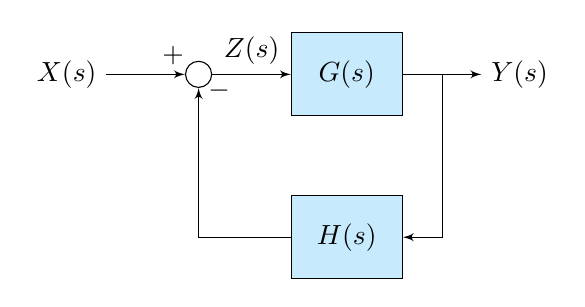
\begin{tikzpicture}[auto, >=latex']
    % Place the blocks
    \node [name=input] {$X(s)$};
    \node [sum, right=of input] (sum) {};
    \node [block, right=of sum] (G) {$G(s)$};
    \node [right=of G] (output) {$Y(s)$};
    \node [block, below=of G] (measurements) {$H(s)$};

    % Connect the nodes
    \draw [arrow] (input) -- node[pos=0.85] {$+$} (sum);
    \draw [arrow] (sum) -- node {$Z(s)$} (G);
    \draw [arrow] (G) -- node [name=y] {} (output);
    \draw [arrow] (y) |- (measurements);
    \draw [arrow] (measurements) -| node[pos=0.99, right] {$-$} (sum);
  \end{tikzpicture}

  \caption{Closed loop block diagram}
  \label{fig:closed_loop_deriv}
\end{figure}

\begin{align}
  Y(s) &= Z(s) G(s) \nonumber \\
  Z(s) &= X(s) - Y(s) H(s) \nonumber \\
  X(s) &= Z(s) + Y(s) H(s) \nonumber \\
  X(s) &= Z(s) + Z(s) G(s) H(s) \nonumber \\
  \frac{Y(s)}{X(s)} &= \frac{Z(s) G(s)}{Z(s) + Z(s) G(s) H(s)} \nonumber \\
  \frac{Y(s)}{X(s)} &= \frac{G(s)}{1 + G(s) H(s)}
\end{align}

A more general form is

\begin{equation}
  \frac{Y(s)}{X(s)} = \frac{G(s)}{1 \mp G(s) H(s)}
\end{equation}

where positive feedback uses the top sign and negative feedback uses the bottom
sign.

\input{app-steady-state-error}
\input{app-luenberger-observer-derivs}
\input{app-integral-control}

% Back matter
\chapterimage{back.jpg}

\backmatter
\glsaddall
\printglossary[title={\sffamily\bfseries Glossary}]
\addcontentsline{toc}{chapter}{\color{deeporange}Glossary}

\chapter{Bibliography}

\phantomsection
\section*{Online}
\addcontentsline{toc}{section}{Online}
\printbibliography[heading=bibempty,type=online]

\phantomsection
\section*{Misc}
\addcontentsline{toc}{section}{Miscellaneous}
\printbibliography[heading=bibempty,type=misc]

% Index
\cleardoublepage
\phantomsection
\addcontentsline{toc}{chapter}{\textcolor{deeporange}{Index}}
\setlength{\columnsep}{0.75cm}
\printindex

\end{document}
